\documentclass[authoryear]{elsarticle}

\setlength\arraycolsep{2pt}
\setlength{\parskip}{1ex plus 0.5ex minus 0.2ex}
\usepackage{graphicx}
\usepackage{amsfonts}
\usepackage{multirow}
\usepackage{comment}

%hello there
%\usepackage{chicago}
\bibliographystyle{chicago}



\newcommand{\eps}{\epsilon}
\newcommand{\var}{{\rm var}}
\newcommand{\cov}{{\rm cov}}
\newcommand{\nid}{{\rm NID}}
\newcommand{\diag}{{\rm diag}}
\newcommand{\E}{{\mathrm E}}
\newcommand{\R}{{\mathrm R}}
\newcommand{\RD}{{\tilde{\mathrm R}}}
\newcommand{\Q}{{\mathrm Q}}
\newcommand{\U}{{\mathrm U}}
\newcommand{\Ex}{{\cal E}}
\newcommand{\cor}{\mathrm{cor}}
\newcommand{\tr}{\mathrm{tr}}
\newcommand{\e}{\mathrm{e}}
\newcommand{\de}{\mathrm{d}}
\newcommand{\p}{\mathrm{P}}
\newcommand{\Ln}{\mathrm{Ln}}
\newcommand{\sign}{\mathrm{sign}}

\newcommand{\ra}{\varrho}

\newcommand{\minn}{\mathrm{min}_n}
\newcommand{\maxn}{\mathrm{max}_n}


\newcommand{\cq}{\ ,\quad }
\newcommand{\qq}{\quad \Rightarrow \quad}
\newcommand{\oq}{\quad \Leftarrow \quad}
\newcommand{\eq}{\quad \Leftrightarrow \quad}



\newcommand{\ppo}[1]{|{#1}|^+}

\newcommand{\ssection}[1]{%
  \section[#1]{\textbf{\uppercase{#1}}}}
\newcommand{\ssubsection}[1]{%
  \subsection[#1]{\normalfont\textbf{#1}}}


%\renewcommand{\labelenumi}{(\roman{enumi})}

\newcommand{\eref}[1]{(\ref{#1})}
\newcommand{\fref}[1]{Figure \ref{#1}}
\newcommand{\sref}[1]{\S\ref{#1}}
\newcommand{\tref}[1]{Table \ref{#1}}
\newcommand{\aref}[1]{\ref{#1}}



\newcommand{\bi}{\begin{itemize}}
\renewcommand{\i}{\item}
\newcommand{\ei}{\end{itemize}}


\begin{document}


\begin{frontmatter}

\title{Layer dependence as a measure of local dependence}
\author[acst]{Weihao Choo\corref{cor1}}
\ead{weihao.choo@mq.edu.au}
\author[acst]{Piet de Jong}



\address[acst]{Department of Actuarial Studies Macquarie
University, NSW 2109, Australia.}
\cortext[cor1]{Corresponding author}




\begin{abstract}
This paper introduces, analyses and  illustrates a new measure of local dependence called  ``layer dependence." Layer dependence accurately captures varying dependence in the joint distribution. Layer dependence satisfies coherence properties similar to Spearman's correlation, such as lying between $-1$ and $1$, with $-1$, $0$ and $1$ resulting from countermonotonicity, independence and comonotonicity, respectively. Taking a weighted average of layer dependence values across the joint distribution yields Spearman's correlation and alternative measures of overall dependence. Copulas fitted using layer dependence are tailored to past data and easily incorporate expert opinion on the dependence structure.
\end{abstract}

\begin{keyword}
Local dependence; rank dependence; conditional tail expectation; Spearman's correlation; concordance.
\end{keyword}



\end{frontmatter}

\section{Local dependence and layer dependence}

Dependence between two variables generally varies  with percentile. For example extreme movements in two stock markets are likely be highly related  whereas minor fluctuations may be relatively independent. Natural catastrophes create significant insurance losses for several classes of business at the same time, while attritional losses between various classes are weakly dependent.


Local dependence measures aim to capture the dependence structure of a bivariate distribution. This contrasts with  measures of overall dependence such as Pearson correlation, Spearman's $\rho$ and Kendall's $\tau$ \citep{embrechts2002correlation}. Local dependence measures include the univariate tail concentration \citep{venter2002tails}, correlation curve \citep{bjerve1993correlation}, and bivariate measures by \cite{bairamov2003new}, \cite{jones1996local} and \cite{holland1987dependence}.


This paper introduces, illustrates and analyzes an alternate local dependence measure called  ``layer dependence." Layer dependence is the covariance between a random variable and a single ``layer" of another. Layer dependence is also the ``gap" between upper and lower conditional tail expectations. Random variables are replaced with their percentile rank transforms and layer dependence is calculated entirely from the copula underlying the joint distribution. Hence of interest is rank dependence rather than dependence between random variables in their original scale, as the latter is often distorted by marginal distributions.


Layer dependence satisfies ``coherence" properties similar to linear correlation: between $-1$ and $1$, constant and equal to $-1$, $0$ and $1$ for countermonotonic, independent and comonotonic random variables, sign switching when ranking order reverses, and taking on higher values when dependence is stronger. Taking a weighted average of layer dependence values across the joint distribution yields Spearman's $\rho$ and alternative coherent measures of overall dependence.


Layer dependence provides a more appropriate and accurate measure of local dependence compared to existing measures. Higher dispersion from various points of the $45^\circ$ line reduces layer dependence and vice versa. Calculating layer dependence at the first instance from past data or parametric copula extracts essential and interpretable information -- the dependence structure. For a parametric copula, the implication of its parametric form and parameters on the dependence structure is not always apparent. Similar problems apply when past data is scarce.


Layer dependence offers an alternative approach to copula modeling. First compute layer dependence values from past data, and apply parametric smoothing. Further adjust, if necessary, to incorporate expert opinion. A copula is then fitted to refined layer dependence values. The fitted copula overcomes the inflexibility of parametric copulas to closely capture the dependence structure in past data, whilst avoiding uncertainties of empirical copulas at the other extreme.



The remaining paper is structured as follows. Section \aref{sintroduction} defines and analyzes layer dependence. Section \aref{sldcurve} illustrates layer dependence for several copulas. Section \aref{sdecompose} explains the behaviour of layer dependence by decomposing it into a negative function of discordance and dispersion. Section \aref{scoherence} describes coherence properties of layer dependence. Links to existing literature are highlighted in section \aref{sliterature}. Further properties and expressions of layer dependence are discussed in sections \aref{sproperties} and \aref{sotherexp} respectively. Section \aref{smodeling} suggests approaches to simulate a copula given the layer dependence curve, and section \aref{sfitting} applies layer dependence to copula modeling, using historical stock returns as an illustration. Section \aref{sapplication} discusses further applications of layer dependence, such as forming measures of overall dependence and dependence asymmetry. Section \aref{soriginal} formulates layer dependence in terms of observed random variables instead of their percentile ranks. Section \aref{sconclusion} concludes.

\begin{comment}
The literature suggests several approaches on fitting a copula to past data. If marginal distributions are unknown, a parametric approach typically involves selecting parametric copula and marginal distributions, and estimating parameters by maximising joint likelihood \citep{denuitactuarial}. A semi-parametric approach replaces marginal distributions in joint likelihood with empirical values \citep{oakes1989bivariate}. The choice of parametric copula may be restricted to a specific class of copulas. \cite{genest1993statistical} suggests an approach to select the generator function of Archimedean copulas \citep{mcneil2005qrm}. Alternatively a visual assessment of data may suggest an appropriate parametric copula with similar dependence structure, for example the Gumbel copula if upper tail dependence is present and Clayton copula if lower tail dependence is present. At the other extreme of copula fitting is to use the empirical copula, when the volume of past data is sufficiently large. \citep{czado2010pair} discusses a semi-parametric approach for multivariate copulas, based on vine copulas.
\end{comment}



\section{Layer dependence}\label{sintroduction}

Suppose $u$ and $v$ are percentile ranks of continuous random variables $x$ and $y$.  Then $(u,v)$ has standard uniform marginals and its joint distribution $C$ is a copula \citep{nelson1999ic}.

This paper defines and discusses a new form of local dependence between $u$ and $v$, called ``layer dependence." Of interest is rank dependence rather than dependence between $x$ and $y$ which is influenced by marginal distributions of $x$ and $y$. Layer dependence exploits the decomposition
\begin{equation}\label{decompose}
u=\int_0^1 (u>\alpha) \de \alpha =  \int_0^u \de \alpha \ ,
\end{equation}
where $(u>\alpha) \de \alpha$ is the ``$\alpha$--layer'' of $u$ and $(u>a)$ is the indicator function:  $1$ if $u>\alpha$ and $0$ otherwise. Given $\alpha$, the derivative of $\alpha$--layer with respect to $u$ is $1$ when $u=\alpha$ and $0$ otherwise. This implies $\alpha$--layer reflects movements in $u$ at $\alpha$, and ignores movements elsewhere. Thus $u$, from \eref{decompose}, is formed from infinitely many layers, each layer capturing the variability of $u$ at a different point.

The $\alpha$--layer dependence  between $v$ and the $\alpha$--layer of $u$ is defined in terms of covariance calculations
\begin{equation}\label{definition}
\ell_\alpha \equiv \frac{\cov\{v,(u>\alpha)\}}{\cov\{u,(u>\alpha)\}}
=\frac{\cor\{v,(u>\alpha)\}}{\cor\{u,(u>\alpha)\}} \cq 0\leq\alpha\leq 1\;,
\end{equation}
where cov and cor calculate covariance and correlation, respectively, using $C$. Denominators in \eref{definition} are independent of $C$ and forces $\ell_\alpha=1$ if $u=v$ and $\ell_\alpha=-1$ if $u=1-v$. Hence $\alpha$--layer dependence $\ell_\alpha$ measures dependence between $v$ and $u$ at $\alpha$. Further $-1\leq \ell_\alpha \leq 1$. Independence implies $\ell_\alpha=0$. Coherence properties of $\ell_\alpha$ are formalised in section \aref{scoherence}.

Expanding covariance terms in \eref{definition} and manipulating yields
\begin{equation}\label{gapexp}
\ell_\alpha = \frac{\E(v|u>\alpha)-\E(v|u\leq \alpha)}{\E(u|u>\alpha)-\E(u|u\leq \alpha)}
=2 \left\{\E(v|u>\alpha)-\E(v|u\leq \alpha)\right\}\;,
\end{equation}
where $\E$ calculates expectations with respect to $C$. The first expression in \eref{gapexp} is the expected change in $v$ relative to the expected change in $u$ when $u$ cross $\alpha$. The latter is $0.5$ regardless of $\alpha$, yielding the second expression in \eref{gapexp}. Hence large $\ell_\alpha$ implies $v$ is sensitive to movements in $u$ across $\alpha$, indicating strong dependence between $v$ and $u$ at $\alpha$. When $\ell_\alpha=0$, $v$ is unchanged on average when $u$ crosses $\alpha$, hence $u$ and $v$ are independent at $\alpha$.


Using \eref{decompose} and \eref{definition}, write Spearman's correlation between $u$ and $v$ as
\begin{equation}\label{wtdaverage}
\rho_S\equiv \cor(u,v) =\frac{\cov(u,v)}{\var(u)}=\frac{\int _0^1\cov\{v,(u>\alpha)\}\de\alpha}{1/12}
=\Ex(\ell_\alpha)\; .
\end{equation}
where the expectation $\Ex$ is calculated over $0\le\alpha\le 1$ using density $6\alpha(1-\alpha)$. Hence Spearman's correlation averages $\alpha$--layer dependence using a certain density on $\alpha$. The density integrates to $1$, has minimum $0$ at $\alpha=0$ and $1$, and increases symmetrically to $1.5$ at $\alpha=0.5$. Varying the density leads to different emphasis on different areas of the relationship between $u$ and $v$, and yields alternative measures of overall dependence. For example using the density $n\alpha^{n-1}$ where $n>0$ puts increasing weight on upper tail dependence. This is further discussed in section \aref{sapplication}.



\begin{comment}
  Further alternative expressions are
$\ell_\alpha = (\tau_\alpha-1)/\alpha$ and $\tau_\alpha= (1+\alpha\ell_\alpha)/2$
where  $\tau_\alpha\equiv \E(v|u>\alpha)$.  These  alternative expressions for $\ell_\alpha$ follow from
$$
\cov\{v,(u>\alpha)\} =\frac{(2\tau_\alpha-1)(1-\alpha)}{2}
\cq
\cov\{u,(u>\alpha)\} =\frac{\alpha(1-\alpha)}{2}\ .
$$

Further
$$
\cor\{v,(u>\alpha)\}=\frac{\cov\{v,(u>\alpha)\}}{\sqrt{\alpha(1-\alpha)/12}}  = \ell_\alpha \sqrt{3\alpha(1-\alpha)}\ .
$$
\end{comment}



\section{Layer dependence curves for various copulas}\label{sldcurve}

The nine panels in \fref{fillustration} display $(u,v)$ scatterplots of symmetric copulas, and their layer dependence curves: $\ell_\alpha$ over $0\le\alpha\le1$. Each copula has Spearman's correlation $\rho_S=0.6$.

Each $\ell_\alpha$ curve reflects the dependence structure between $u$ and $v$. Given $\alpha$, $\ell_\alpha$ is larger if points are more clustered around $(\alpha,\alpha)$ and vice versa, as formalised in section \aref{sdecompose}. In addition, $\ell_\alpha$ increases to $1$ in the tails where points converge to the $45^\circ$ degree line indicating perfect dependence.

The nine panels in \fref{fillustration} highlight the inadequacies of using Spearman's correlation to measure overall dependence, particularly in the tails. In contrast, layer dependence curves capture the dependence structure of each copula.


\begin{figure}
  \begin{center}
    \begin{tabular}{ccc}
      \resizebox{40mm}{!}{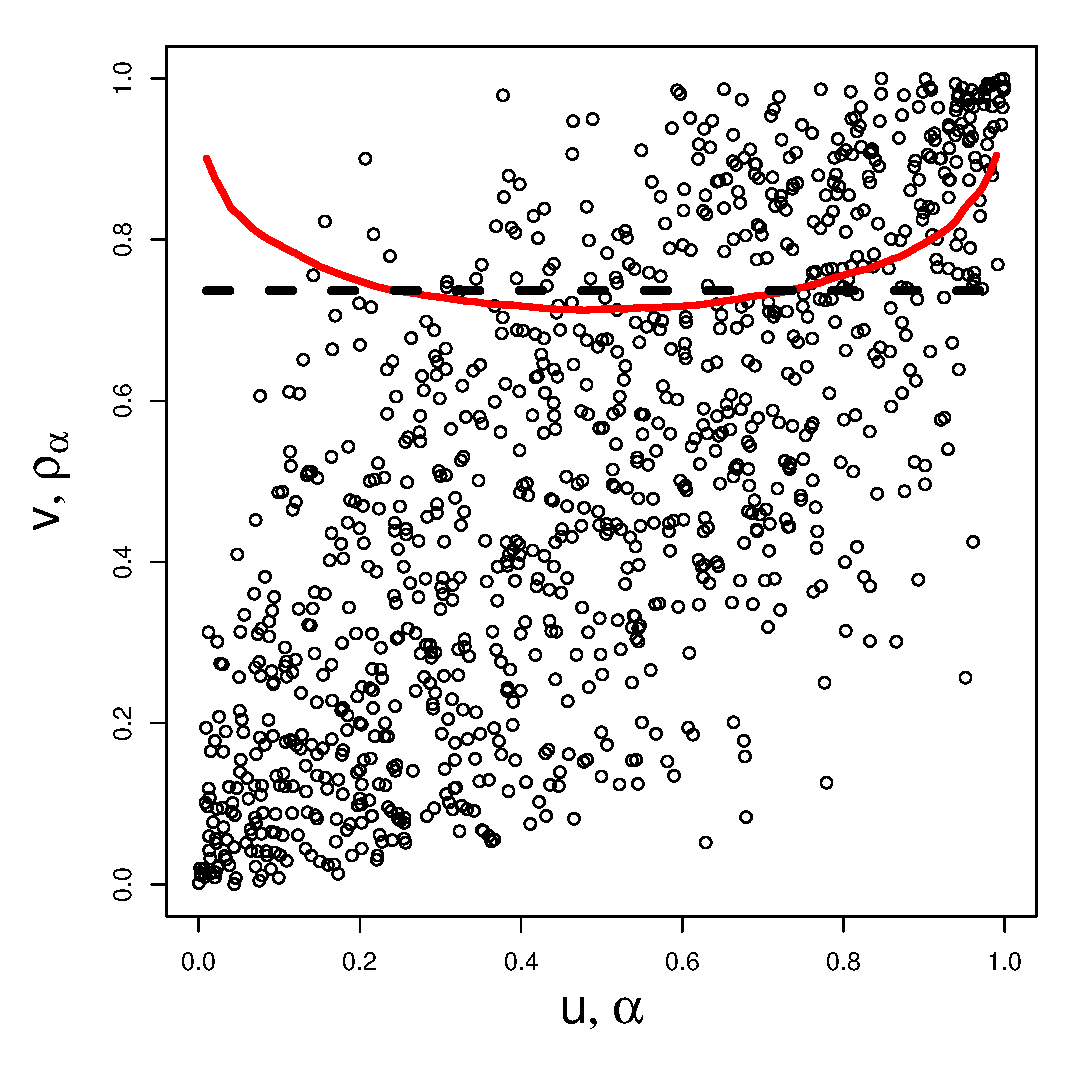
\includegraphics{normal.eps}}
            \resizebox{40mm}{!}{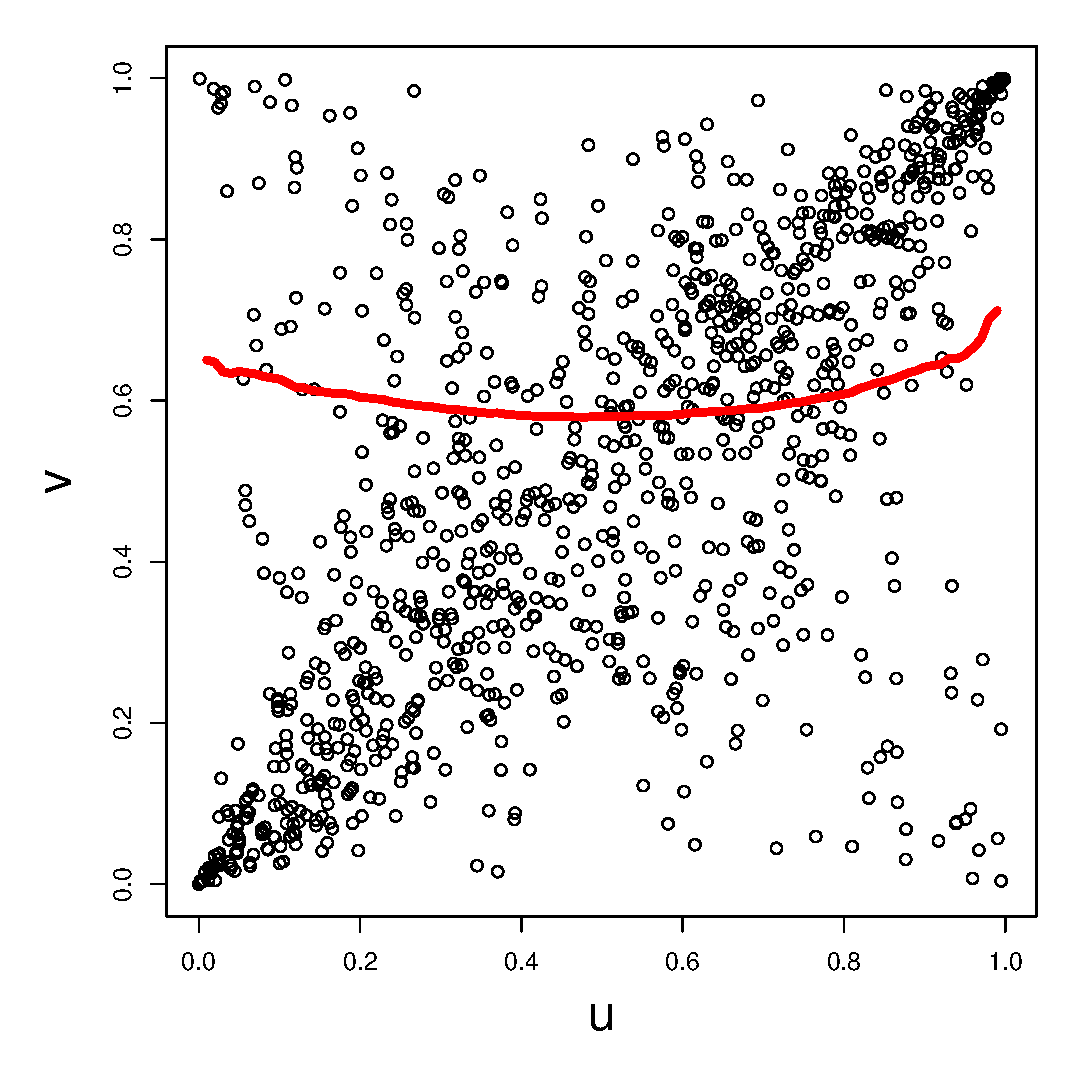
\includegraphics{student.eps}}
      \resizebox{40mm}{!}{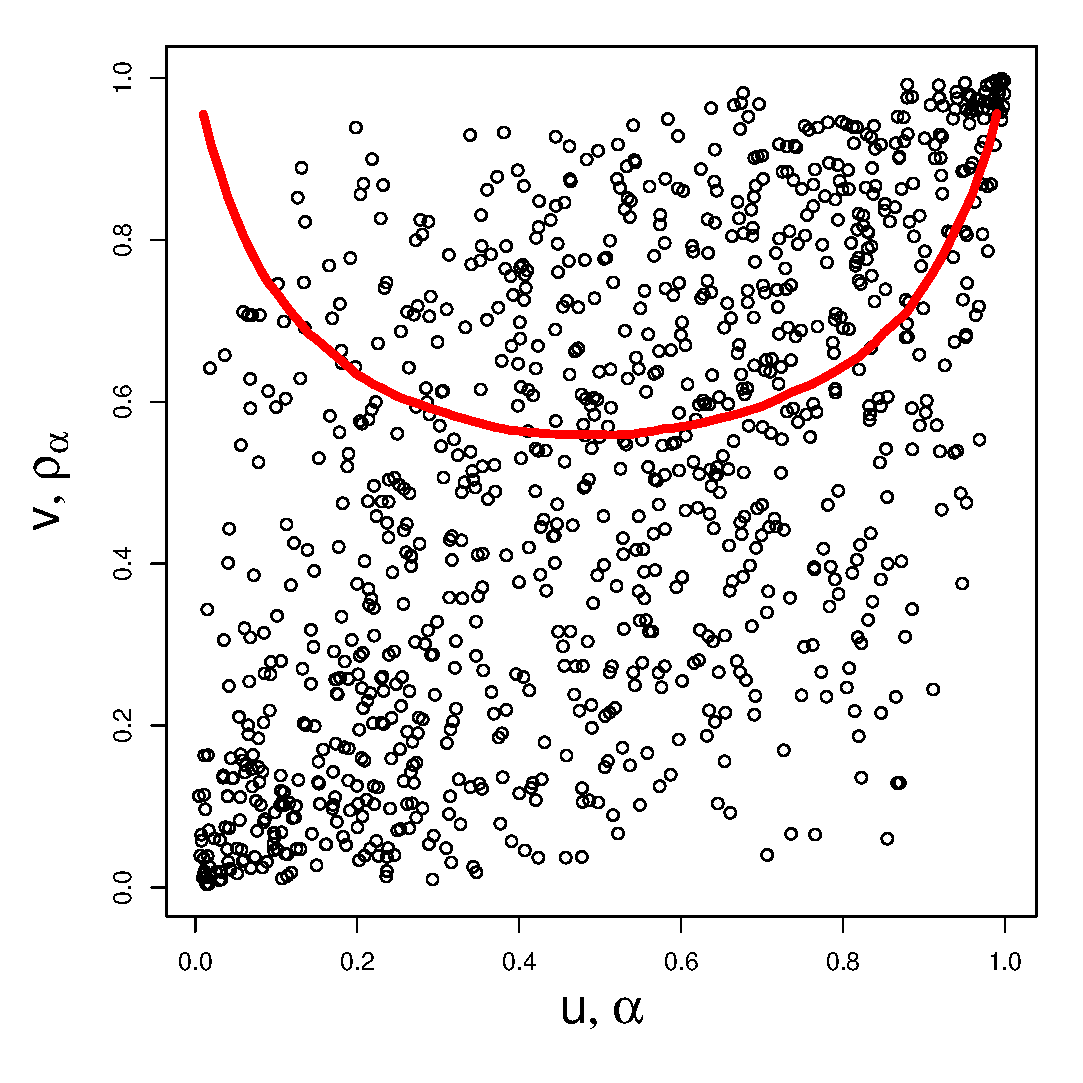
\includegraphics{structural2.eps}} \\
      \resizebox{40mm}{!}{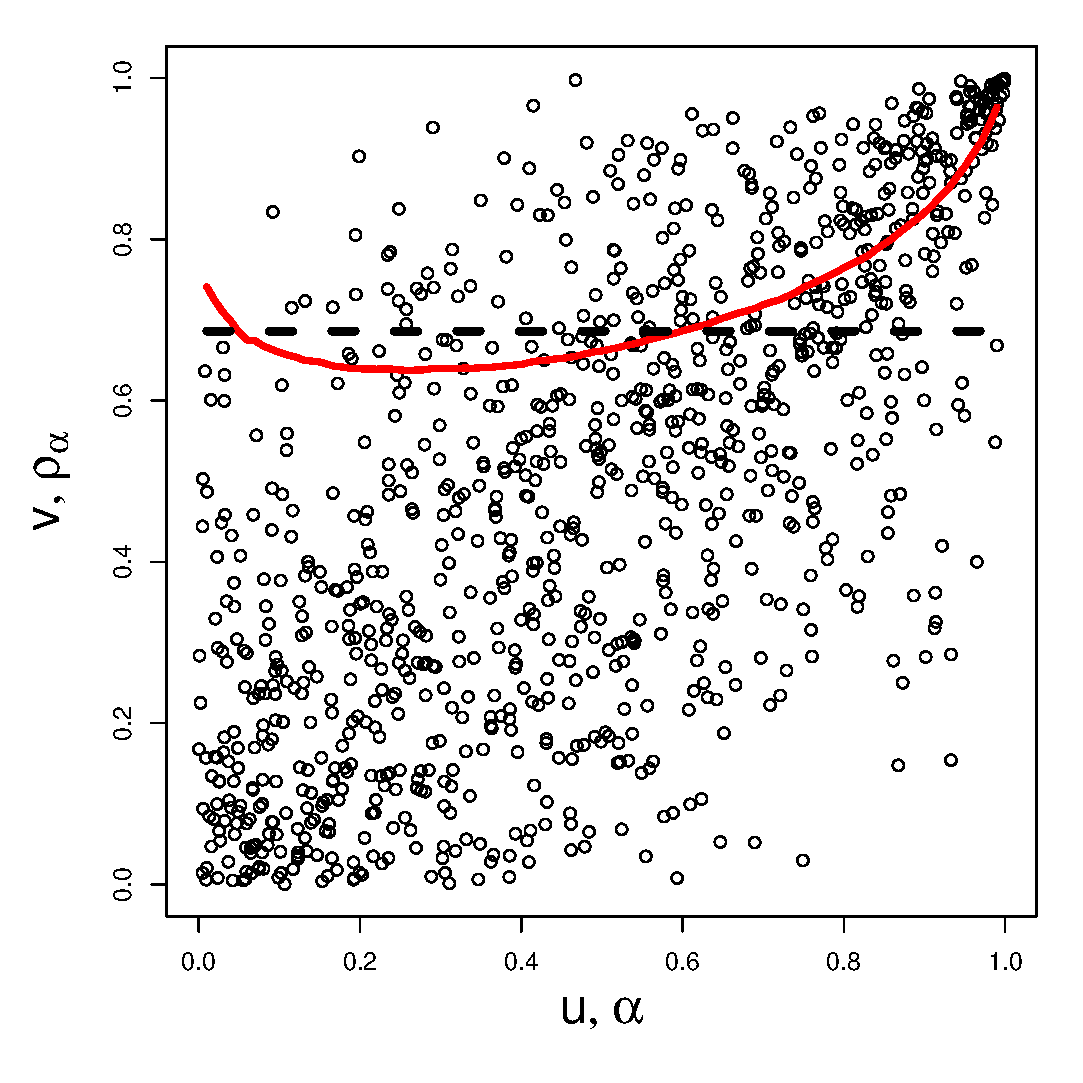
\includegraphics{gumbel.eps}}
            \resizebox{40mm}{!}{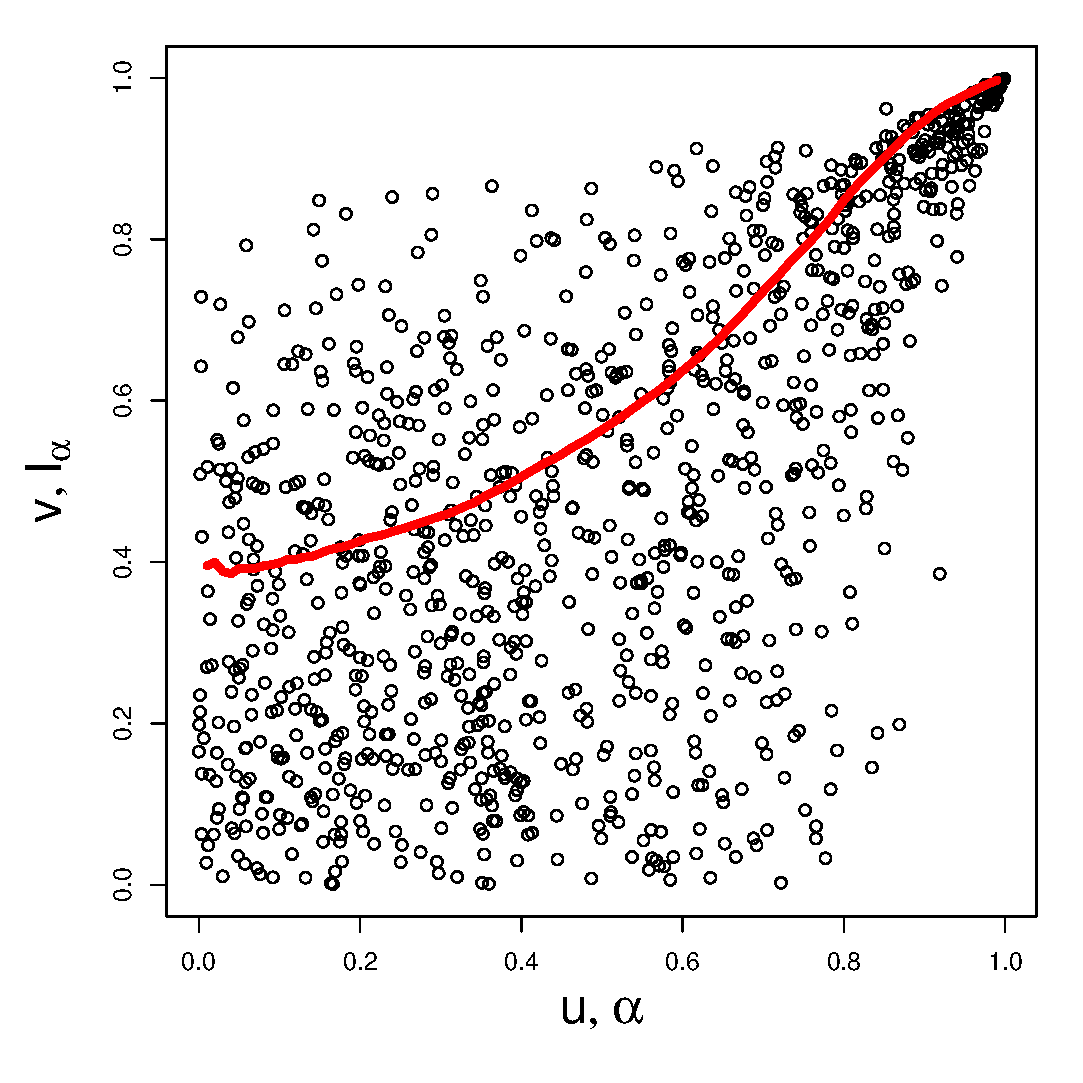
\includegraphics{structural1.eps}}
      \resizebox{40mm}{!}{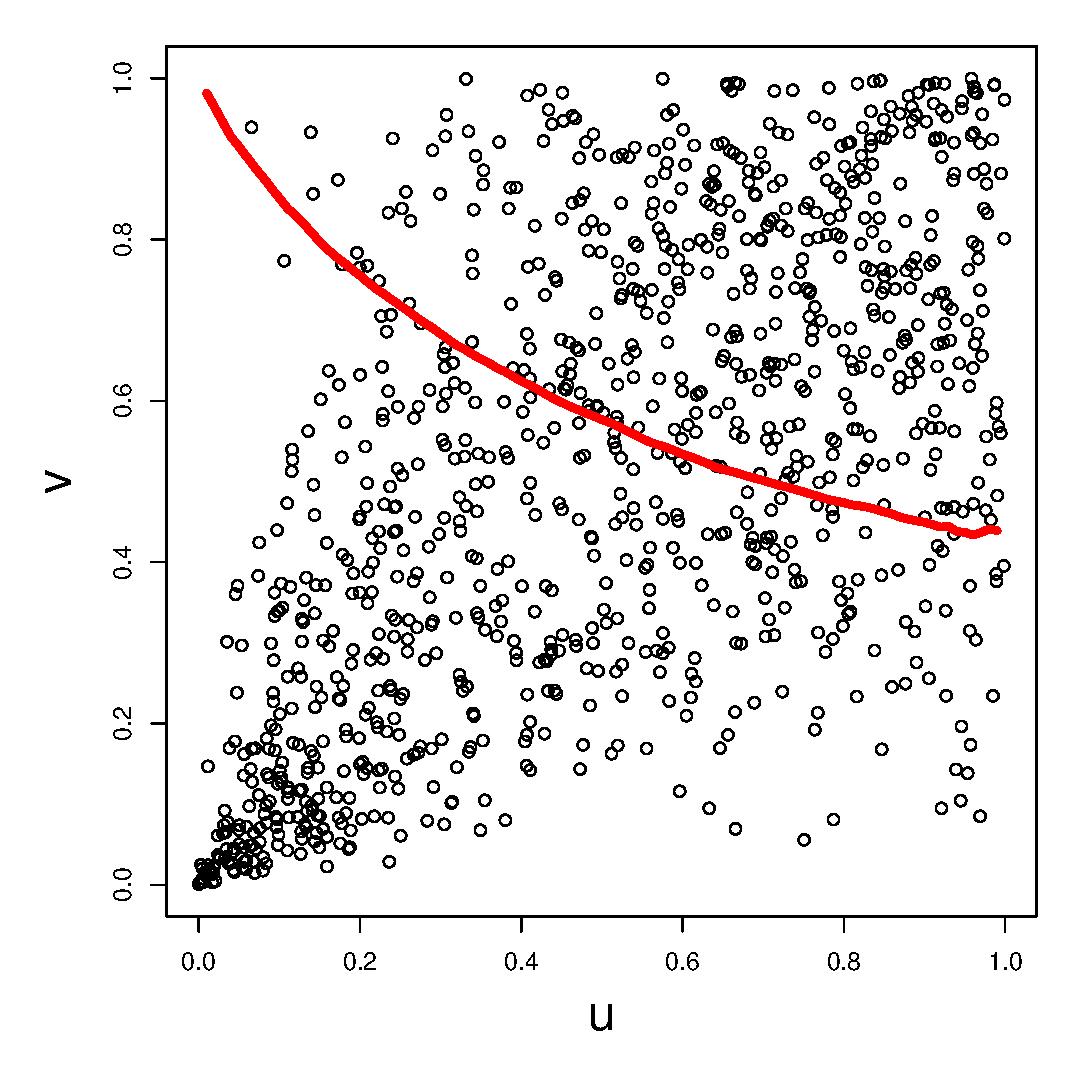
\includegraphics{clayton.eps}} \\
            \resizebox{40mm}{!}{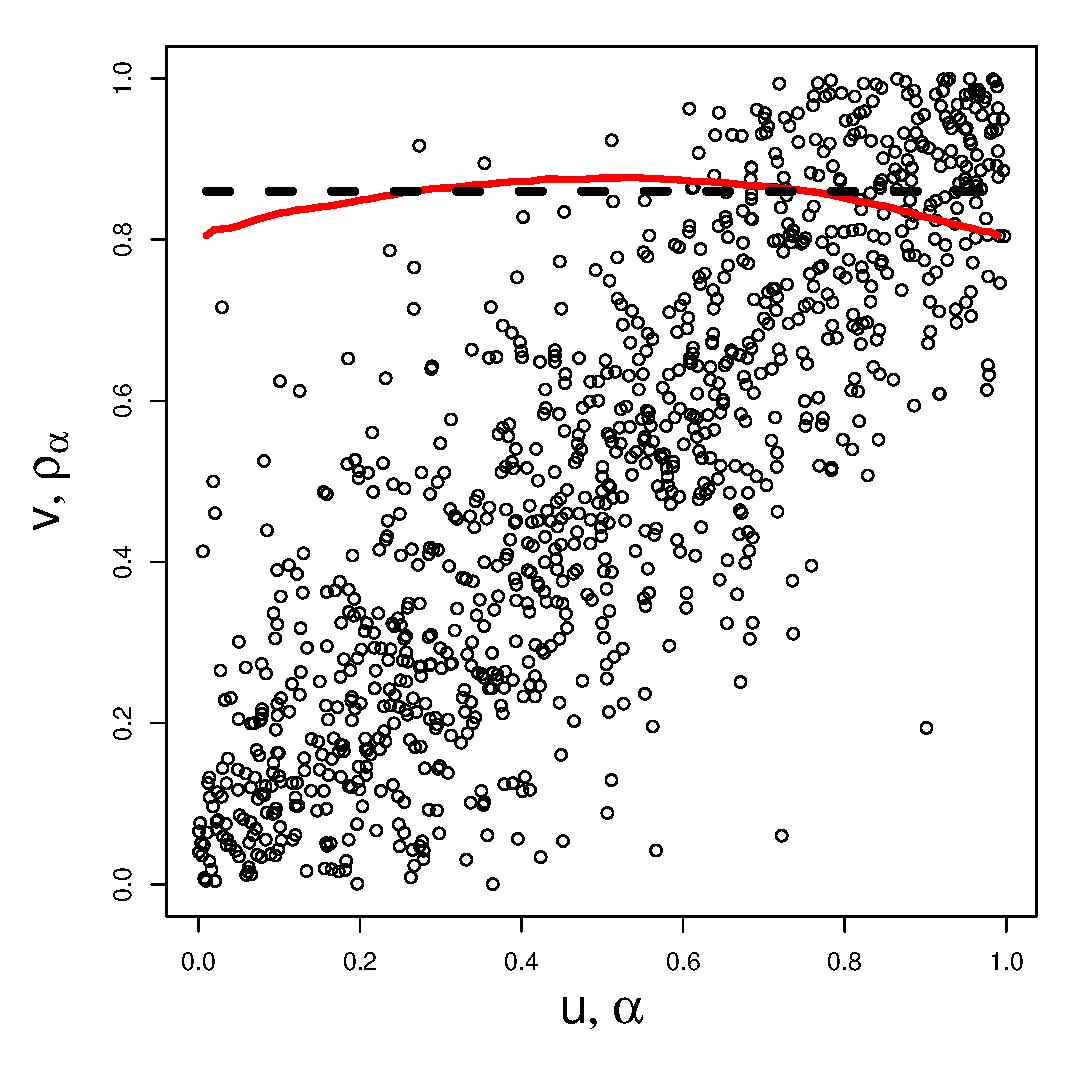
\includegraphics{frank.eps}}
            \resizebox{40mm}{!}{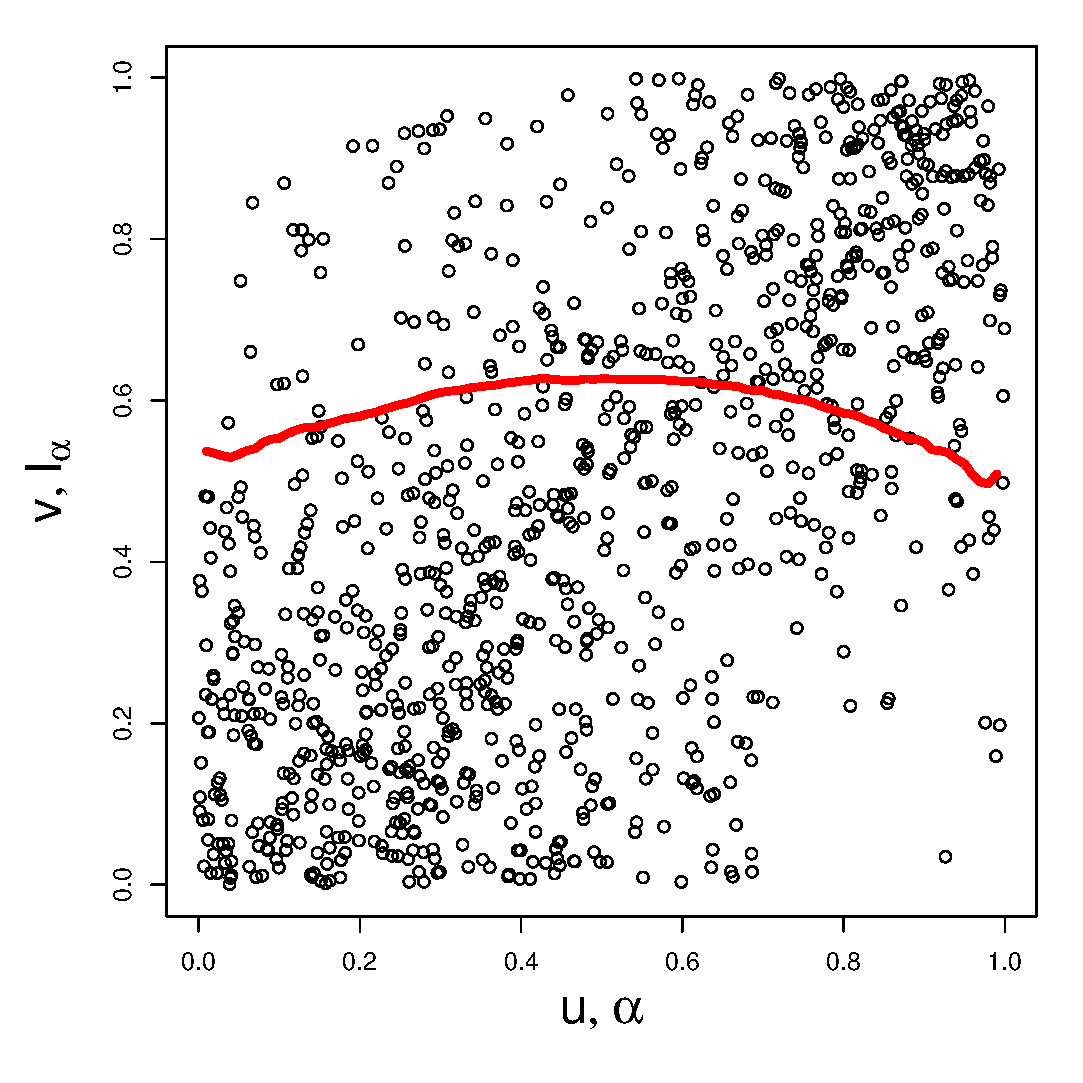
\includegraphics{structural3.eps}}
      \resizebox{40mm}{!}{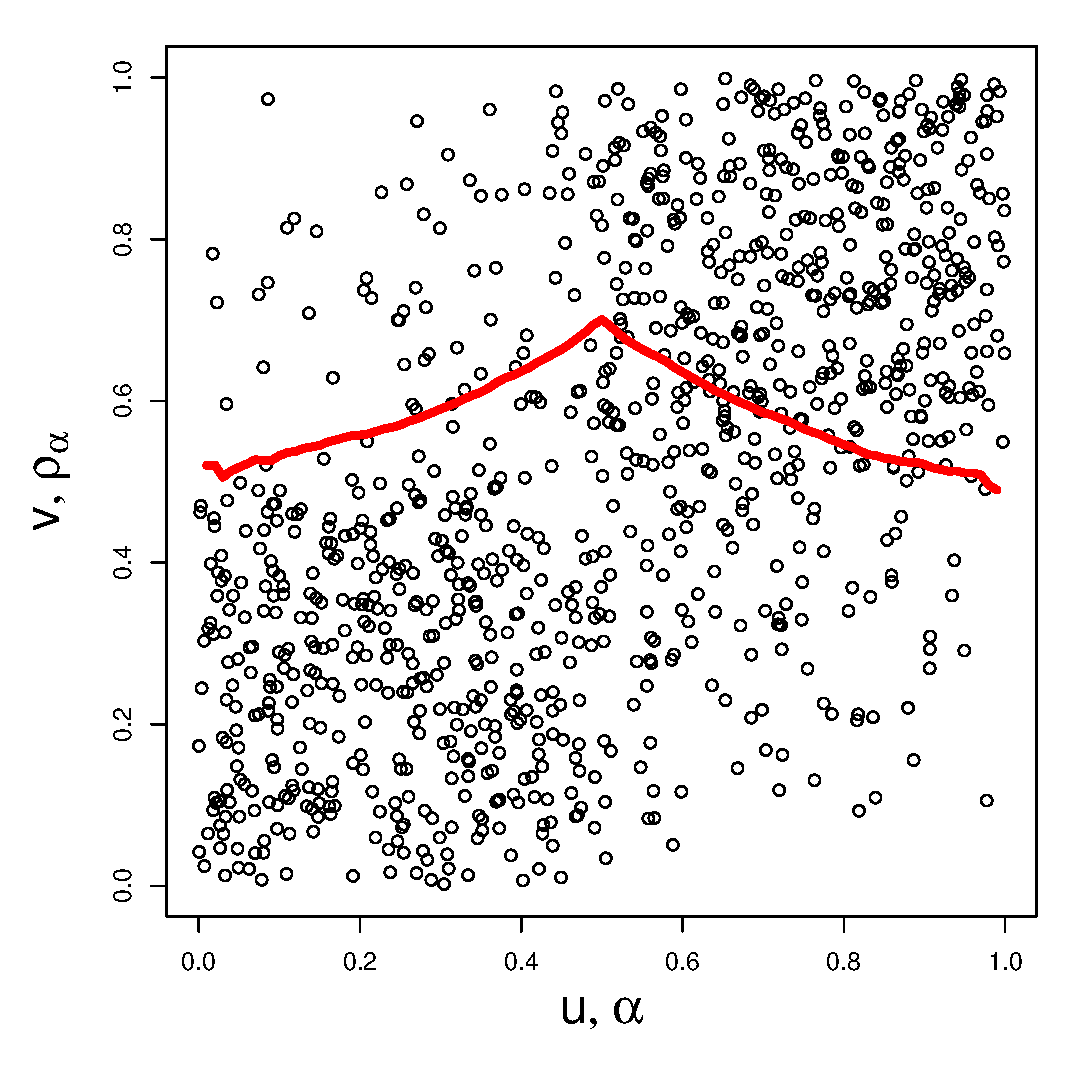
\includegraphics{structural4.eps}} \\
    \end{tabular}
    \caption{Copulas with different layer dependence curves $\ell_\alpha$ over $0\lq\alpha\le 1$ (red curves) but the same  $\rho_S=0.6$.}
    \label{fillustration}
  \end{center}
\end{figure}



\section{Layer dependence, discordance and dispersion}\label{sdecompose}

If $(u,v)$ is exchangeable,  $C(u,v)=C(v,u)$, then layer dependence $\ell_\alpha$ measures the lack of discordance and dispersion at $\alpha$:
\begin{equation}\label{decomposition}
\ell_\alpha = 1-2(1+\gamma_\alpha) \delta_\alpha \;,
\end{equation}
where
$$
\gamma_\alpha \equiv \cor\{(u\leq\alpha),(v>\alpha)\} =\cor\{(u>\alpha),(v\leq\alpha)\}\;,
$$
$$
\delta_\alpha \equiv\E\left\{(|u-v|)|(u-\alpha)(v-\alpha)<0\right\}  \; .
$$
A proof of \eref{decomposition} is shown below.  The correlation $-1\leq\gamma_\alpha\leq 1$ measures the tendency for $(u,v)$ to be discordant at $\alpha$: opposite signs on $u-\alpha$ and $v-\alpha$, and the expectation $0\leq \delta_\alpha\leq 1$ measures dispersion between values of $u$ and $v$ discordant at $\alpha$.

The proof of \eref{decomposition} follows from
$$
\gamma_\alpha
=-\frac{\cov\{(u\leq\alpha),(v\leq\alpha)\}}{\var\{(u\leq\alpha)\}}
=\frac{\alpha^2-C(\alpha,\alpha)}{\alpha(1-\alpha)}   \;,
$$
and
$$
\delta_\alpha = 2 \E\left\{(u-v)(u>v)|(u-\alpha)(v-\alpha)<0\right\}
$$
$$
=  \frac{2\E\{(u-v)(u>v)(u>\alpha)(v\leq\alpha)\}}{2\E\{(u>\alpha)(v\leq\alpha)\}}
= \frac{\E\{(u-v)(u>\alpha)(v\leq\alpha)\}}{\alpha-C(\alpha,\alpha)}
$$
$$
= \frac{\E\{(u-v)(u>\alpha)\}-\E\{(u-v)(u>\alpha)(v>\alpha)\}}{\alpha-C(\alpha,\alpha)}
 = \frac{\E\{(u-v)(u>\alpha)\}}{\alpha-C(\alpha,\alpha)} \;.
$$
Substituting the above expressions for $\gamma_\alpha$ and $\delta_\alpha$ into the right hand side of \eref{decomposition} yields the expression for $\ell_\alpha$ in \eref{gapexp}, completing the proof.

Result \eref{decomposition} explains the behaviour of layer dependence curves in \fref{fillustration}. Layer dependence $\ell_\alpha$ is larger if there are fewer discordant pairs at $\alpha$, and discordant pairs at $\alpha$ are closer to the $45^\circ$ degree line. The former indicates smaller $\gamma_\alpha$ and the latter indicates smaller $\delta_\alpha$. Vice versa for small $\ell_\alpha$. If $\ell_\alpha=1$ then $\gamma_\alpha=-1$ or $\delta_\alpha=0$, implying $u$ and $v$ are simultaneously below or above $\alpha$ and $u=v$ for discordant pairs. If $\ell_\alpha=1$  in an interval, then $u=v$  in the same interval.

\fref{finterpretation} illustrates the relationship between layer dependence, discordance and dispersion in \eref{decomposition} using two copulas with $\ell_\alpha=1$ and $\ell_\alpha=0.86$ at $\alpha=0.75$. When $\ell_\alpha=1$, there is no discordance or dispersion at $\alpha$. As $\ell_\alpha$ decreases from $1$, the number of discordant pairs and their dispersion increases.

\begin{figure}
  \begin{center}
    \begin{tabular}{cc}
      \resizebox{60mm}{!}{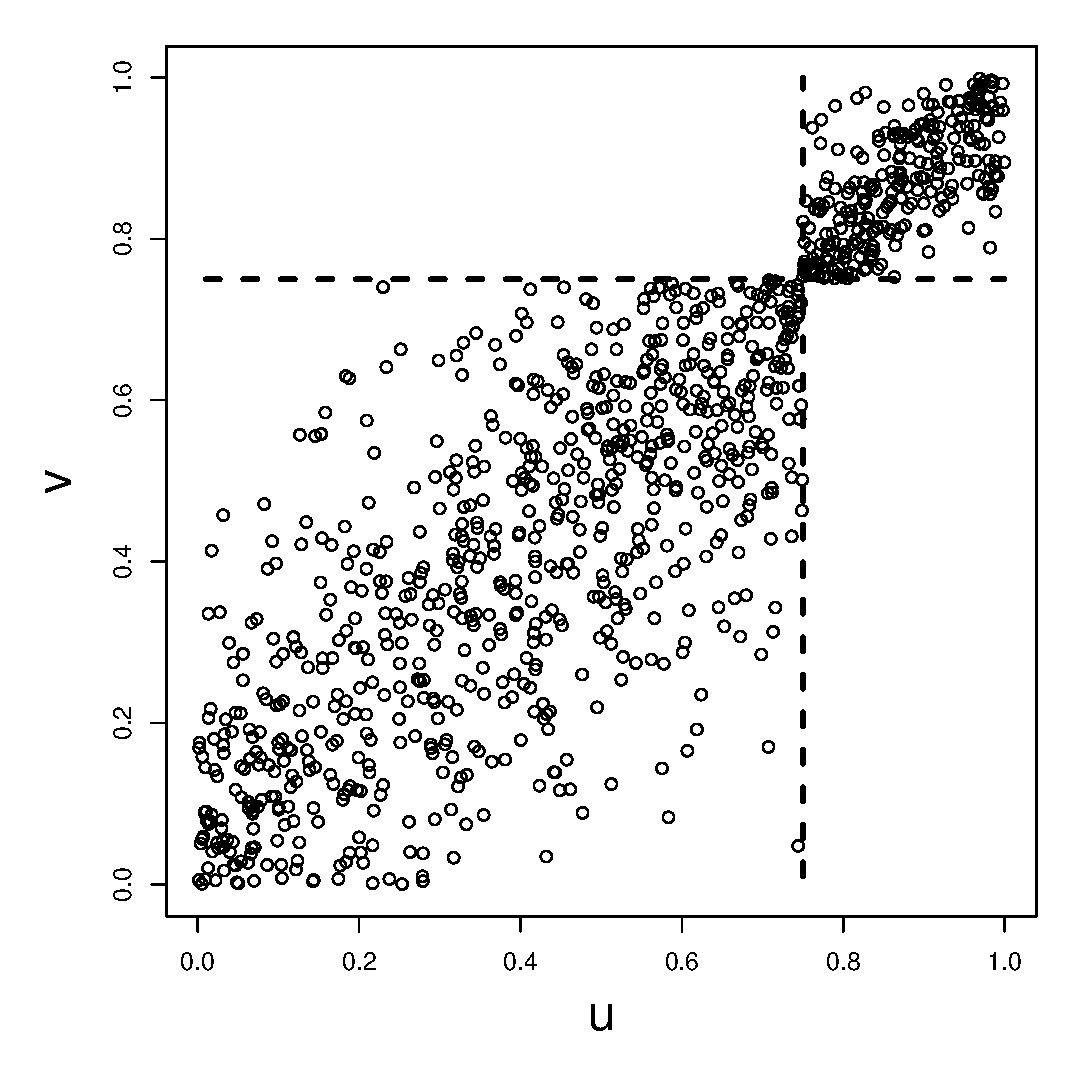
\includegraphics{perfect.eps}}
      \resizebox{60mm}{!}{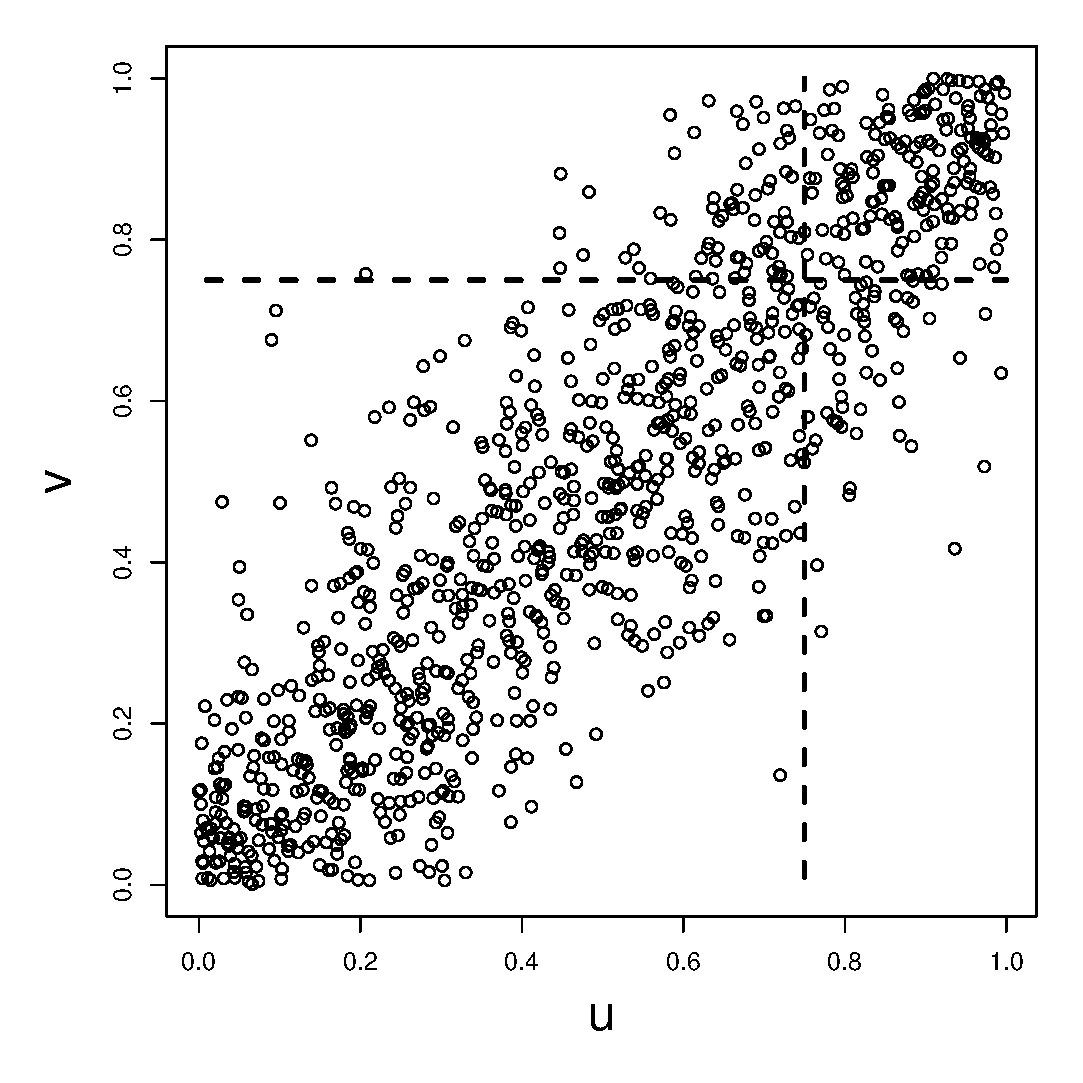
\includegraphics{imperf.eps}} \\
    \end{tabular}
    \caption{The left and right panel  show $\ell_{0.75}=1$ and $\ell_{0.75}=0.86$, respectively. In the left panel, $\gamma_{0.75}=-1$ and $\delta_{0.75}=0$. In the right panel, $\gamma_{0.75}=-0.65$ and $\delta_{0.75}=0.21$.  }
    \label{finterpretation}
  \end{center}
\end{figure}







\begin{comment}

The probability of discordance is
$$
\E[\{(u-\alpha)(v-\alpha)<0\}]
=2\alpha\{(1-\alpha)(\gamma_\alpha+\alpha^2)-1\} \;.
$$


The following illustrates \eref{decomposition} using the income-education example introduced in \sref{sintroduction}. Given $\alpha$, classify individuals as ``concordant" or ``discordant." The former are those with income and education both below or above $\alpha$. The latter are remaining individuals. Scale the proportion of concordant individuals to yield $\gamma_\alpha^*$. Calculate average dispersion $\delta_\alpha$ as twice the average difference between income and education of discordant individuals. Combine $\gamma^*_\alpha$ and $\delta_\alpha$ using \eref{decomposition} to yield $\alpha$-layer dependence $\ell_\alpha$. Layer dependence decreases with the proportion of discordant individuals and their average income-education dispersion.




\fref{fdecomposition} illustrates the decomposition of percentile rank gap by separately showing the standardised concordance probability $\gamma_\alpha^*$ and dispersion $\delta_\alpha$. The same four copulas as in \fref{fillustration} are applied.

\begin{figure}
  \begin{center}
    \begin{tabular}{cc}
      \resizebox{60mm}{!}{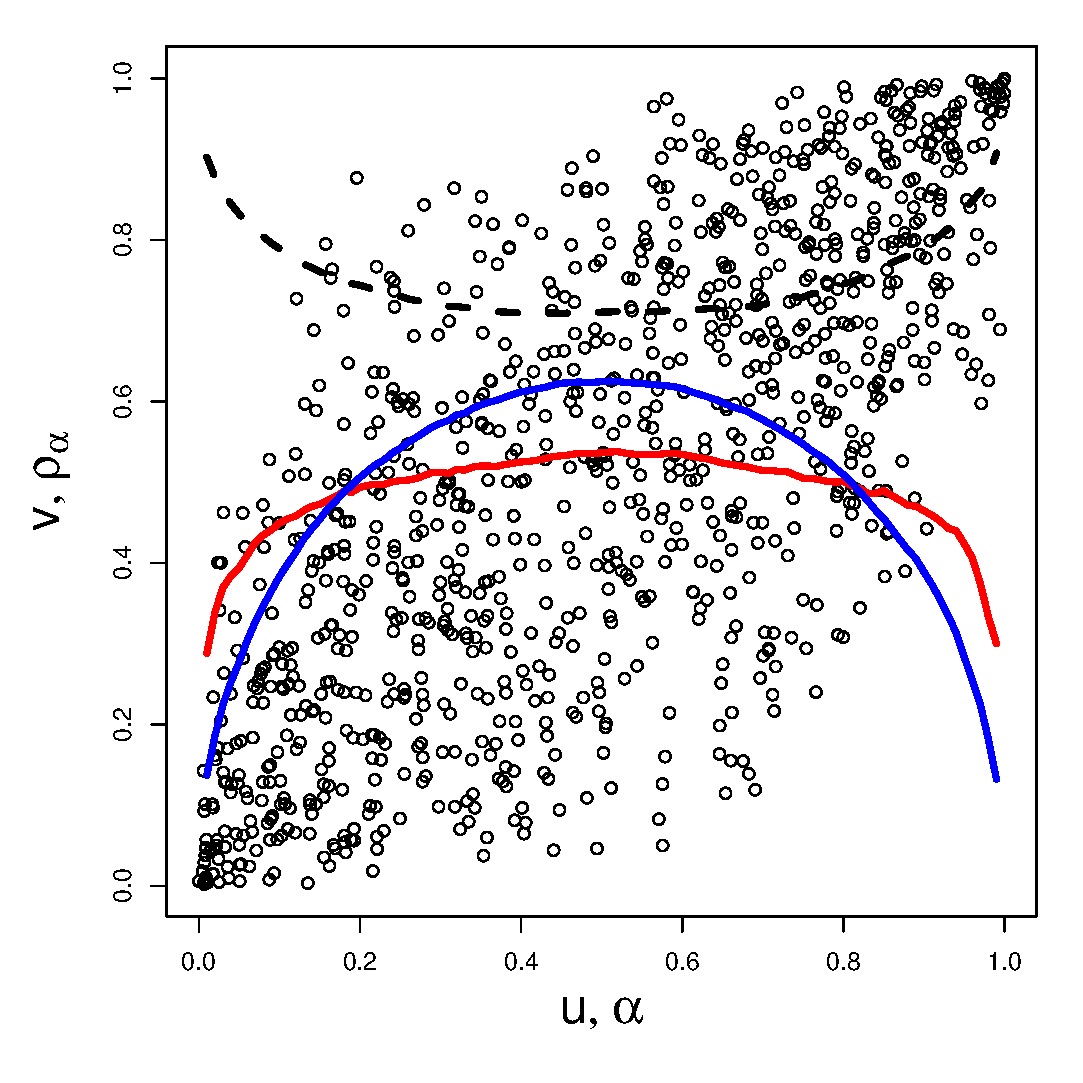
\includegraphics{normaldecom.eps}}
      \resizebox{60mm}{!}{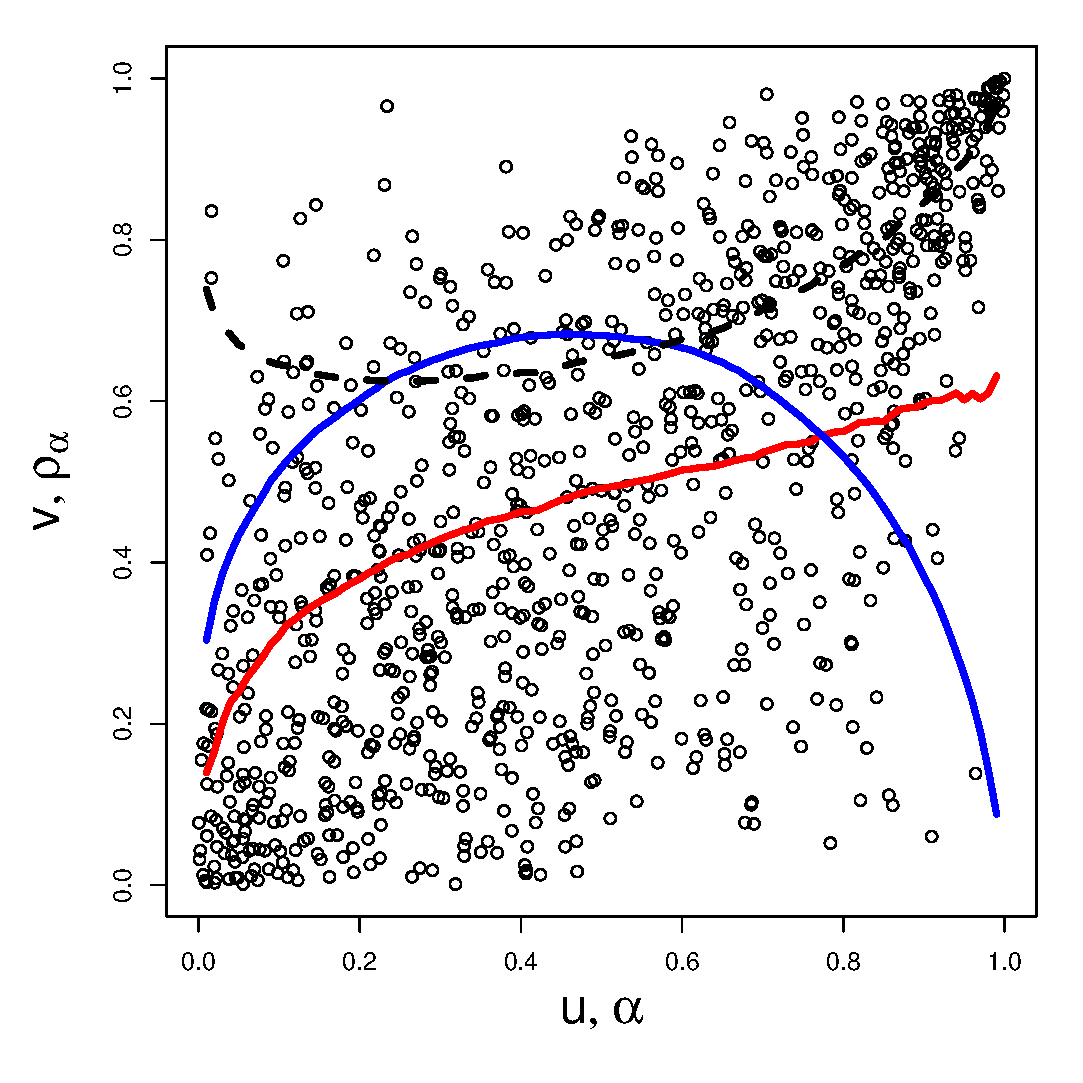
\includegraphics{gumbeldecom.eps}} \\
      \resizebox{60mm}{!}{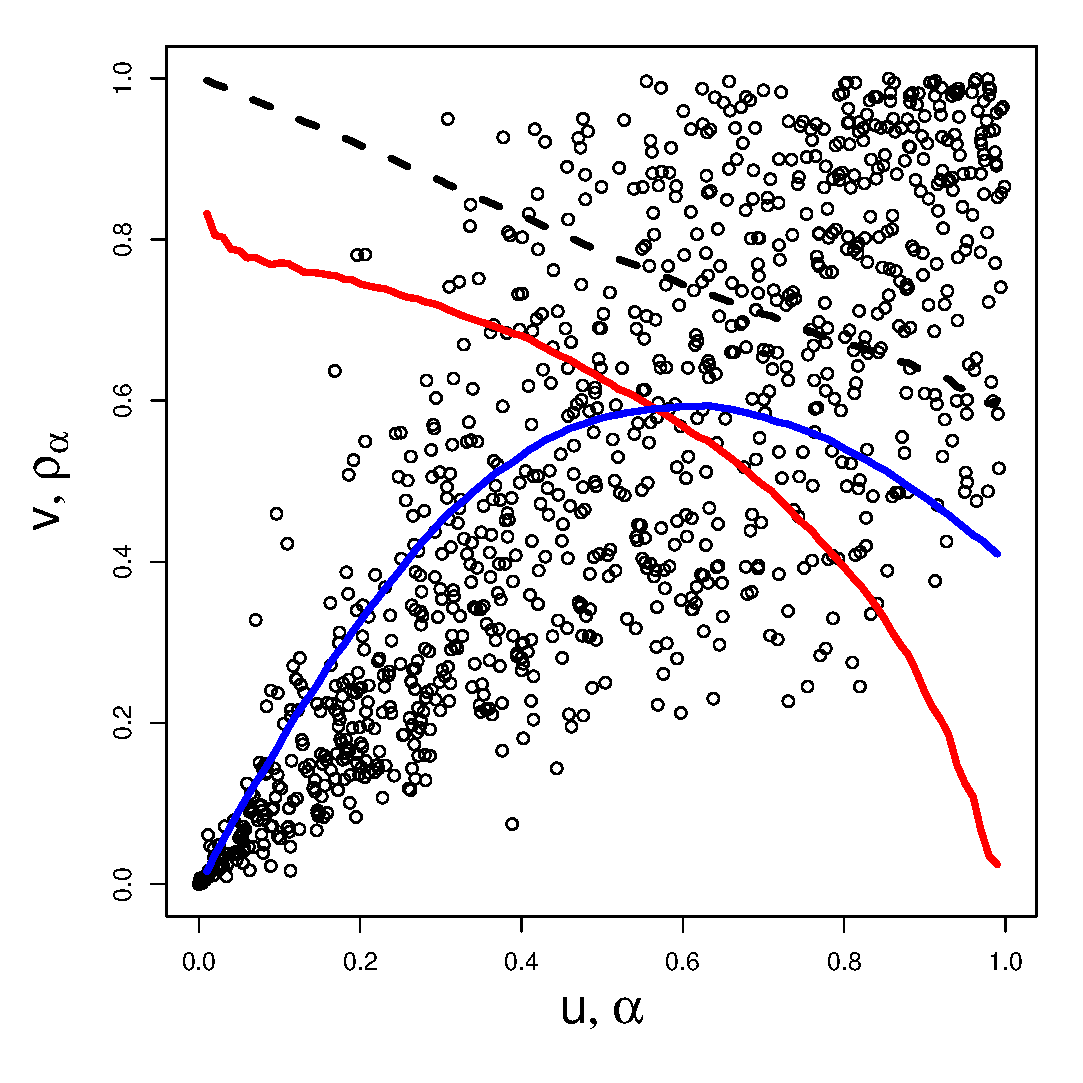
\includegraphics{claytondecom.eps}}
      \resizebox{60mm}{!}{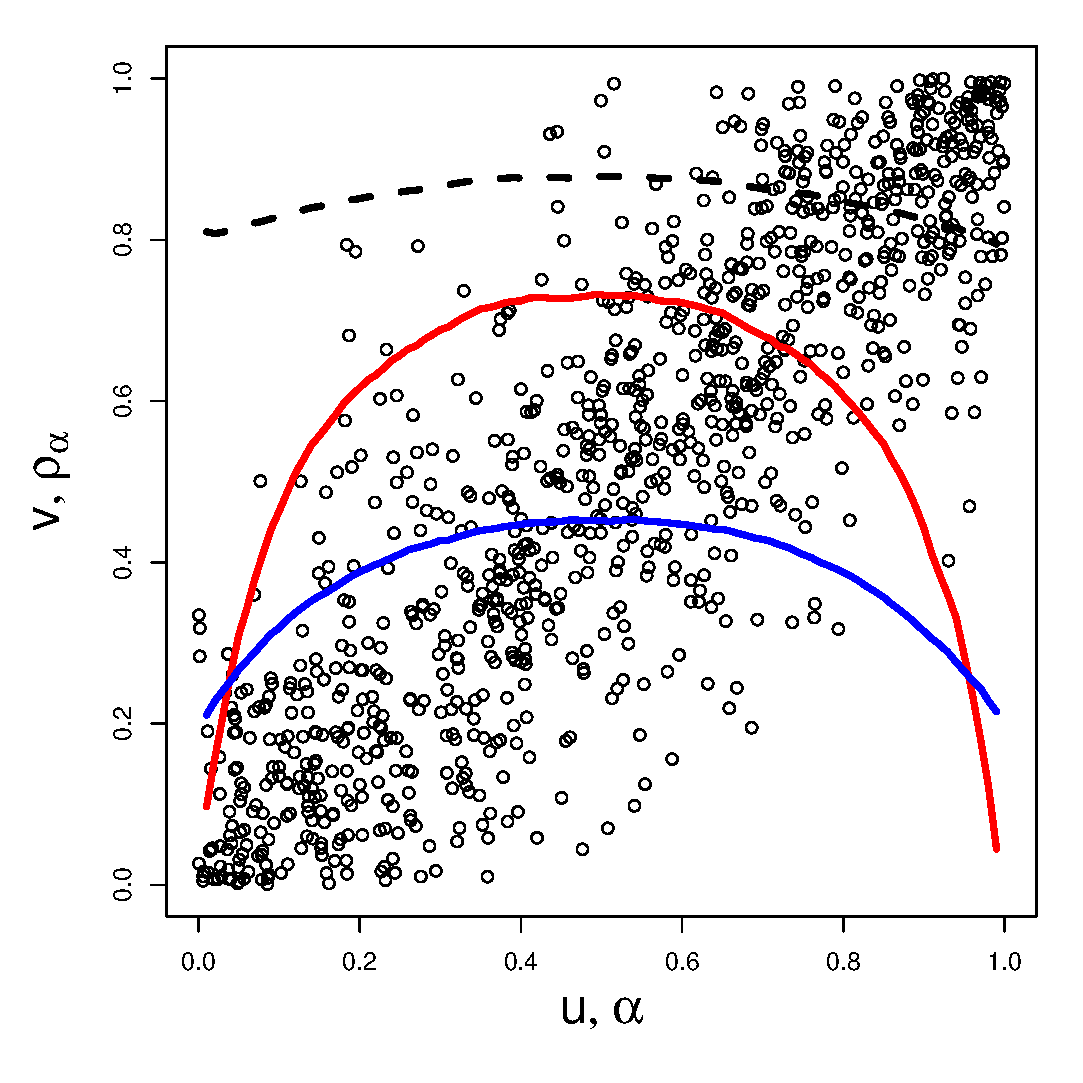
\includegraphics{frankdecom.eps}} \\
    \end{tabular}
    \caption{Standardised concordance probability $\sgamma^*_\alpha$ (red line) and dispersion $\delta_\alpha$ (blue line) for a Gaussian copula (top left), Gumbel copula (top right), Clayton copula (bottom left) and Frank copula (bottom right). Percentile rank gap (dotted black line) is also shown.}
    \label{fdecomposition}
  \end{center}
\end{figure}



Manipulating the expression for $\ell_\alpha$ in \eref{relationship} yields
$$
\ell_\alpha = 1- \frac{\E\{d(u,v) z_\alpha\}}{\alpha(1-\alpha)}  \cq \ell = 1-6\int_0^1 \E\{d(u,v)z_\alpha\} \de \alpha \;.
$$
where the above result for $\ell$ applies $\ell=\int_0^1 w_\alpha \ell_\alpha \de \alpha$, $w_\alpha\equiv 6\alpha(1-\alpha)$. Hence $\rho_S$ is negatively related to the average dispersion between discordant $(u,v)$ over all $\alpha$.






========== Haven't done much below here =============

\subsection{Income-education interpretation}

The following interprets layer dependence using an income-education example. Consider education $(u)$ and income $(v)$ rankings of individuals in a population, with $0$ and $1$ representing lowest and highest, respectively. Given $\alpha$, divide the population into two segments based on education: $u\leq \alpha$ and $u>\alpha$. Measure average income in each segment. From \eref{gapexp}, $\alpha$-layer dependence is twice the gap in average income between the two segments.

Suppose $\ell_\alpha$ is close to one for $\alpha=0.95$. This implies highly educated individuals (top $5\%$) are likely to be high income earners (top $5\%$), and vice versa. Few individuals have top $5\%$ education and income not in top $5\%$ or vice versa, and their average education-income difference is small. Hence there is strong income-education dependence at the $95$th percentile education layer. Dependence is perfect if $\ell_\alpha=1$. If $\ell_\alpha=0$ then average income is equal between individuals with education below and above top $5\%$, implying independence at the $95$th percentile education layer. The same argument applies to $\ell_\alpha$ for other values of $\alpha$.

This paper formulates layer dependence in terms of $u$ and $v$, in this case income and education ranks. Section \sref{soriginal} discusses an analogous definition of layer dependence between observed random variables $x$ and $y$, or original measurements of income and education.

\end{comment}





\section{Coherence properties of layer dependence}\label{scoherence}


Layer dependence $\ell_\alpha$ satisfies five ``coherence" properties. These properties are  extensions of  properties applying to Spearman's correlation $\rho_S$.
\begin{itemize}

\item \textbf{Bounds}: Layer dependence lies between $-1$ and $1$: $-1 \le\ell_\alpha \le 1$ for all $\alpha$.
Hence layer dependence is bounded in the same way as  $\rho_S$.

\item \textbf{Perfect dependence}: Constant layer dependence of $-1$ or $1$ are equivalent to countermonotonicity and comonotonicity.
Thus $\ell_\alpha=-1$ for all $\alpha$ if and only if  $v=1-u$ while $\ell_\alpha=1$ for all $\alpha$ if and only if  $v=u$.

\item \textbf{Independence}: If $u$ and $v$ are independent then $\ell_\alpha\equiv 0$.   The converse is not true -- zero layer dependence does not imply independence as shown by the following counterexample. Assume $v=u$ and $v=1-u$ with equal probability. Then $\E(v|u=t)=0.5$ for all $0\leq t\leq 1$ implying $\E(v|u>\alpha)=\E(v|u\leq\alpha)=0.5$. Hence $\ell_\alpha=0$. However $u$ and $v$ are not independent.

\item \textbf{Symmetry}: Ranking either $u$ or $v$ in the opposite direction switches the sign of layer dependence. Changing the ranking order of both variables preserves the sign of layer dependence.

\item \textbf{Ordering}: Higher correlation order \citep{dhaene2009correlation} leads to higher layer dependence. Consider bivariate uniform $(u^*,v^*)$ exceeding $(u,v)$ in correlation order: $C^*(a,b)\geq C(a,b)$ for all $0\leq a,b\leq 1$, where $C^*$ is the joint distribution of $(u^*,v^*)$. Then
$
\ell^*_\alpha \geq \ell_\alpha$,   $0\leq\alpha\leq 1$
where $\ell_\alpha^*$ denotes the $\alpha$--layer dependence of $(u^*,v^*)$. Hence greater dependence leads to higher layer dependence.

\end{itemize}
Independence, symmetry and ordering properties follow from the definition of layer dependence in \eref{definition}. From \eref{gapexp}, constant layer dependence of one implies $\E(v|u>\alpha)=(\alpha+1)/2$ and $\E(v|u=\alpha)=\alpha$, for all $0\leq\alpha\leq 1$, hence $v=u$. Similarly constant layer dependence of minus one implies $v=1-u$. The ordering property holds since higher correlation order implies larger covariances \citep{dhaene2009correlation}. Prove the bounds property by combining ordering and perfect dependence properties, and noting countermonotonicity and comonotonicity represent minimum and maximum correlation order, respectively.






\begin{comment}


\subsection{Copula comparison using percentile gap}

The following compares copulas based on their percentile gap values. The comparison yields a goodness-of-fit test when modeling past data using copulas. \fref{comparison} plots upper conditional tail expectations $\E(v|u>\alpha)=0.5(\alpha\ell_\alpha+1)$ of the copulas in \fref{fillustration} against the Gaussian copula. Given $\alpha$, points above the $45^{o}$ line indicates the copula has percentile gap exceeding that of the Gaussian copula. Vice versa for points below the $45^{o}$ line.


 we can easily simulate $\tau_\alpha$ paths as $(1/2)+\e^{(1-\alpha)}+\eps_\alpha$.

\begin{figure}
  \begin{center}
    \begin{tabular}{ccc}
      \resizebox{40mm}{!}{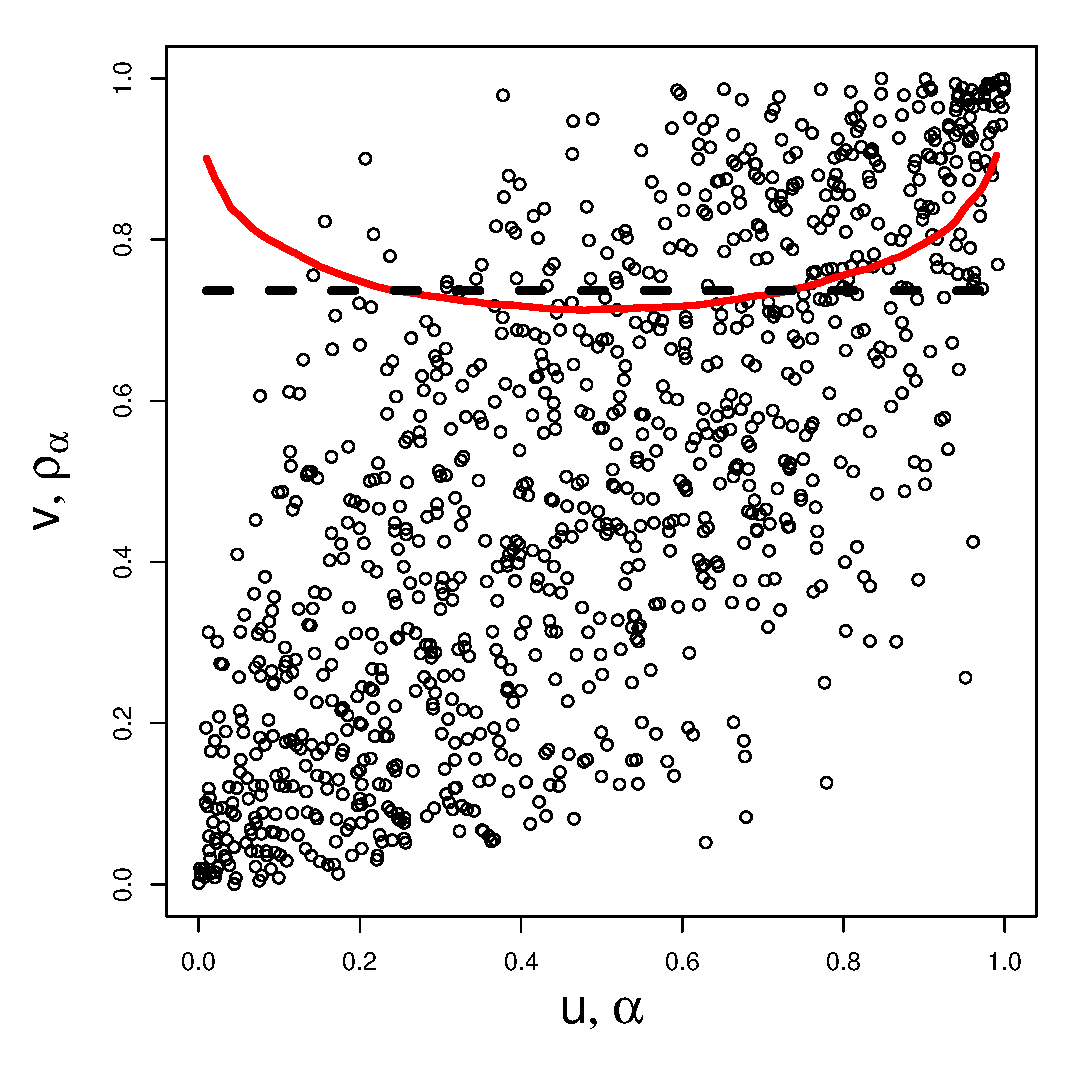
\includegraphics{normal.eps}}
            \resizebox{40mm}{!}{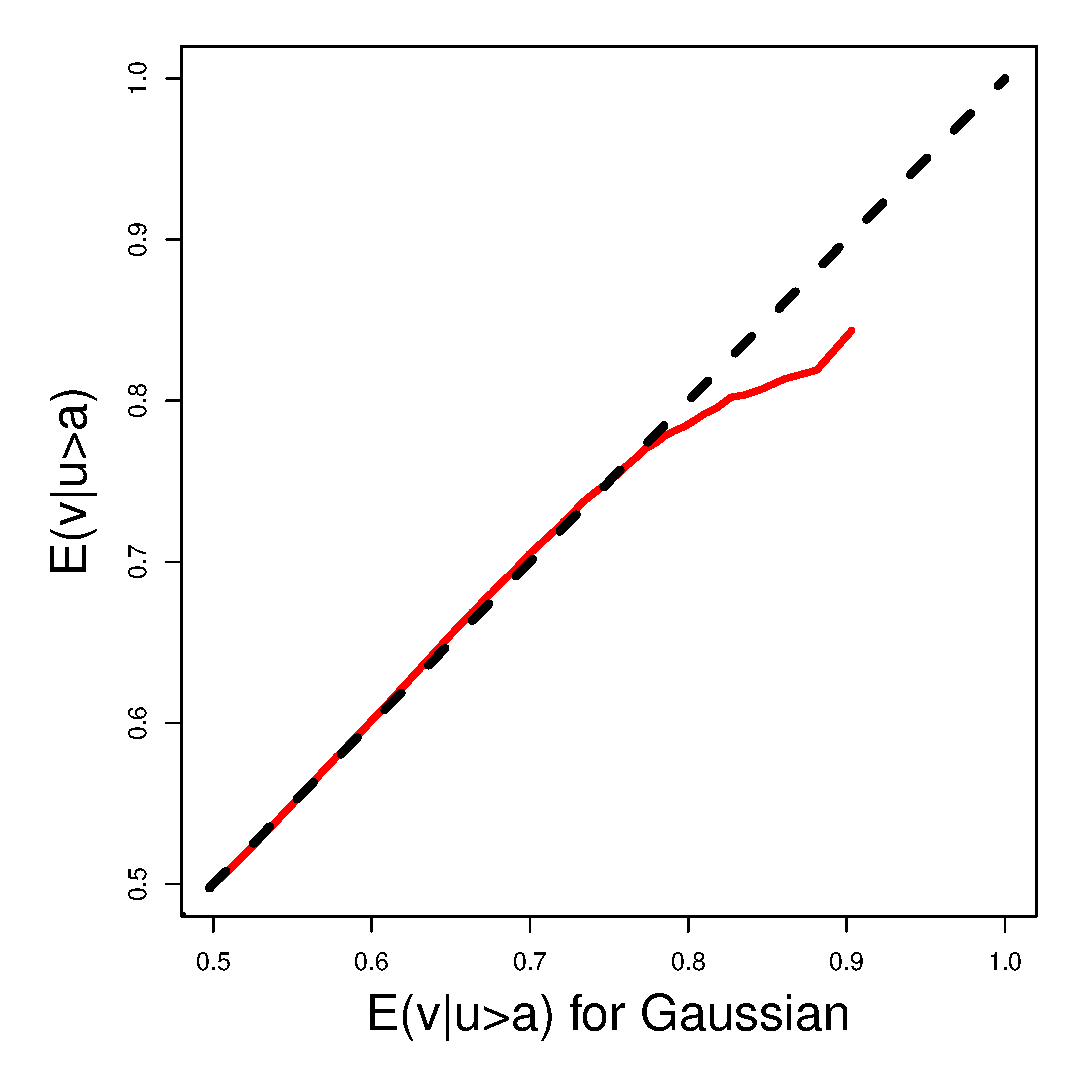
\includegraphics{studentvs.eps}}
      \resizebox{40mm}{!}{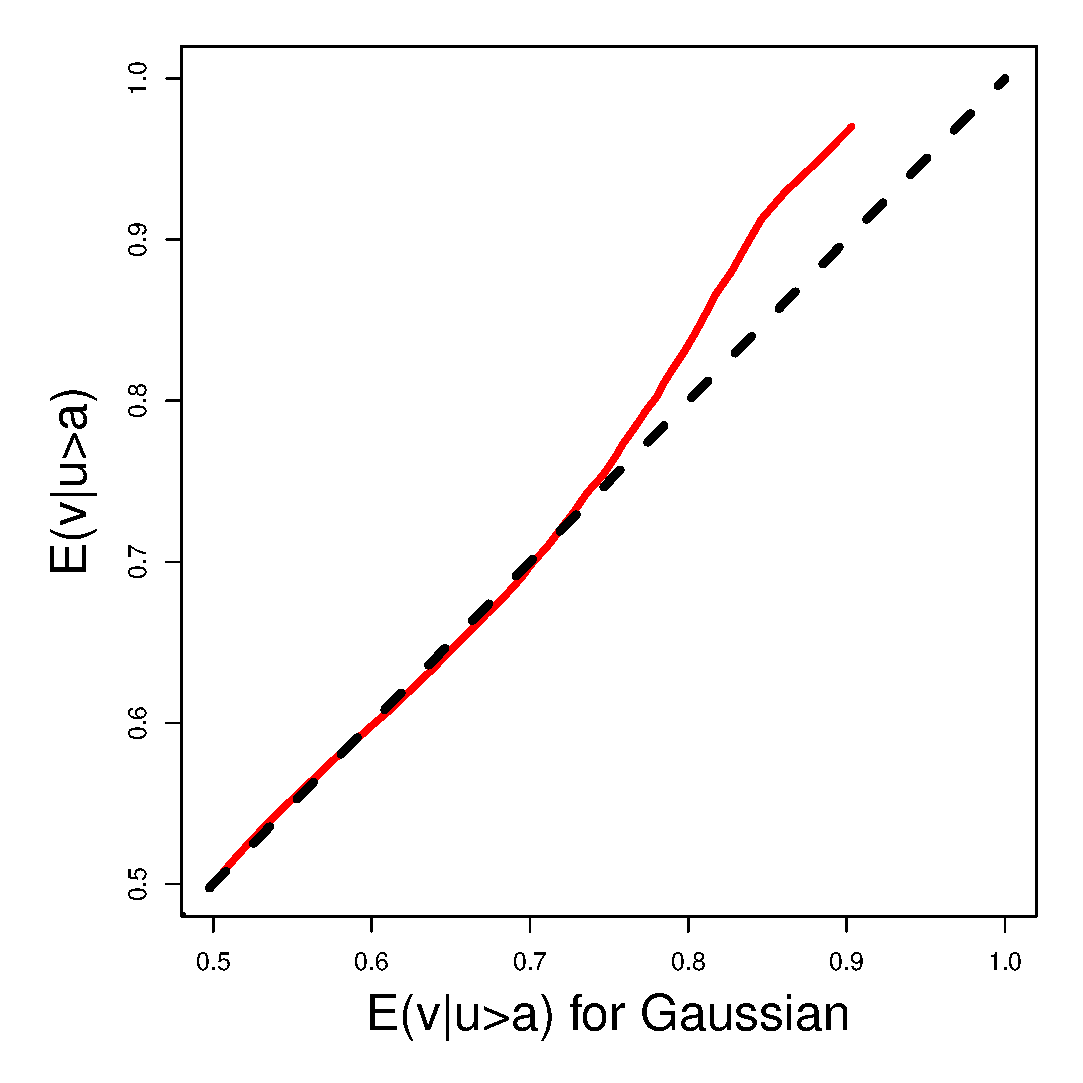
\includegraphics{structural2vs.eps}} \\
      \resizebox{40mm}{!}{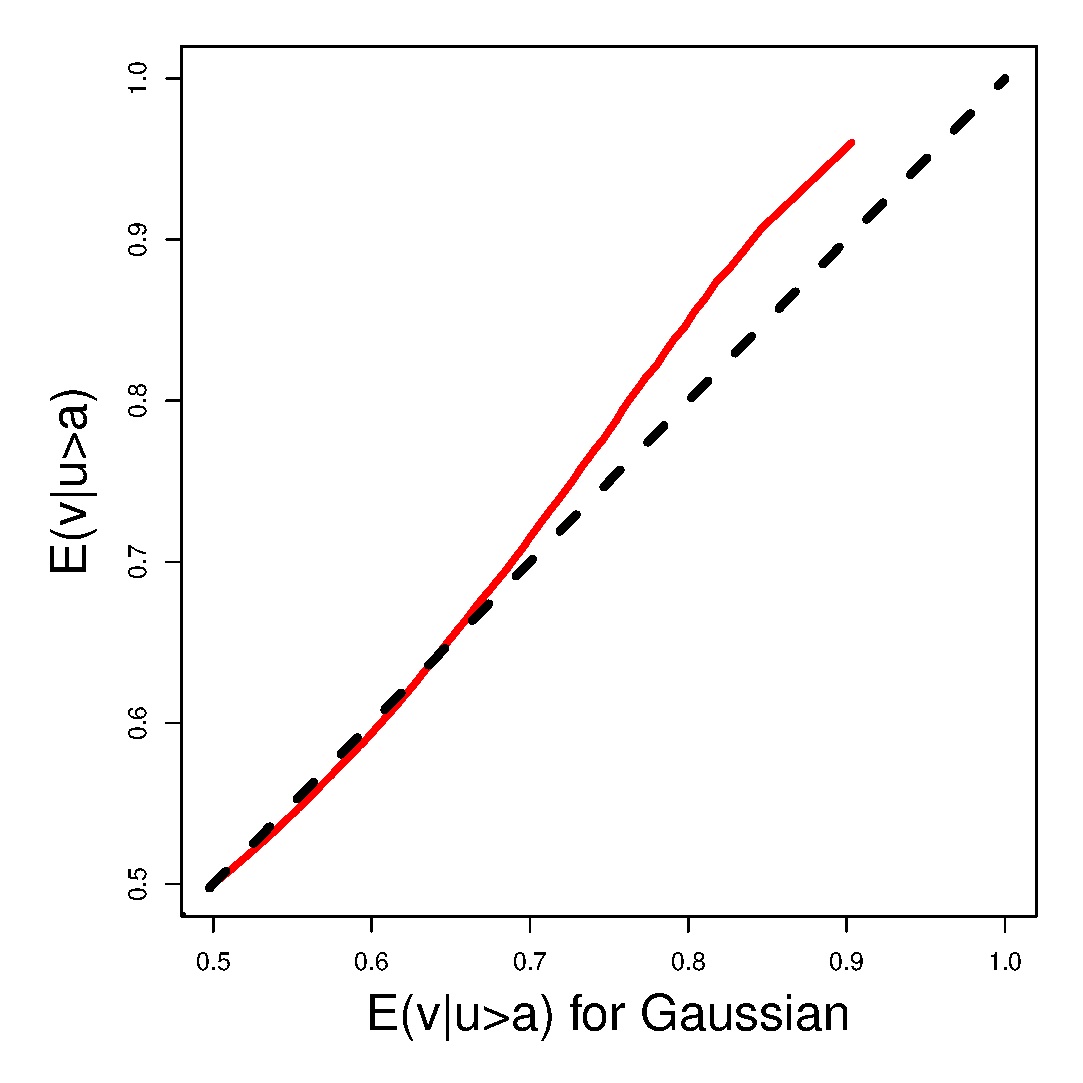
\includegraphics{gumbelvs.eps}}
            \resizebox{40mm}{!}{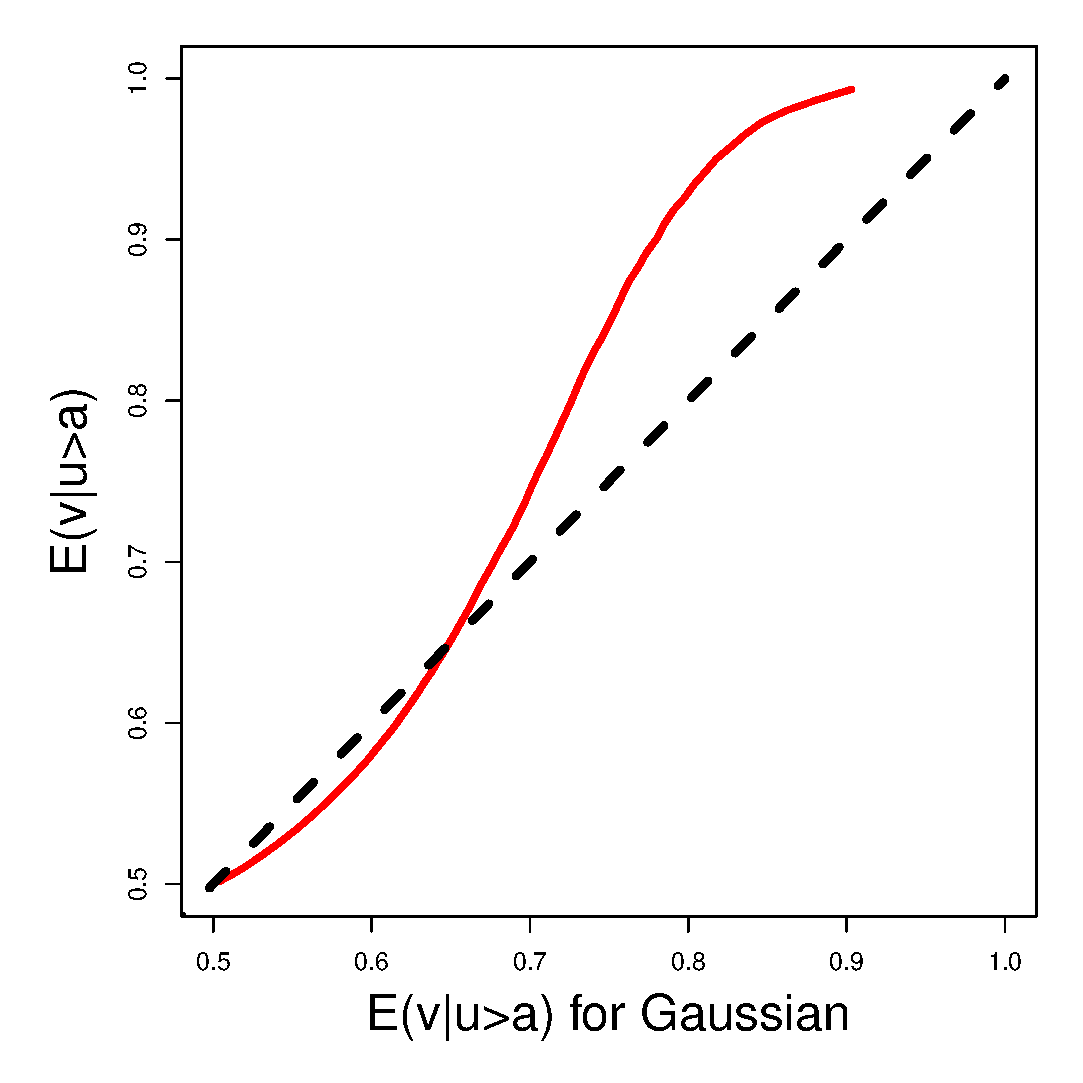
\includegraphics{structural1vs.eps}}
      \resizebox{40mm}{!}{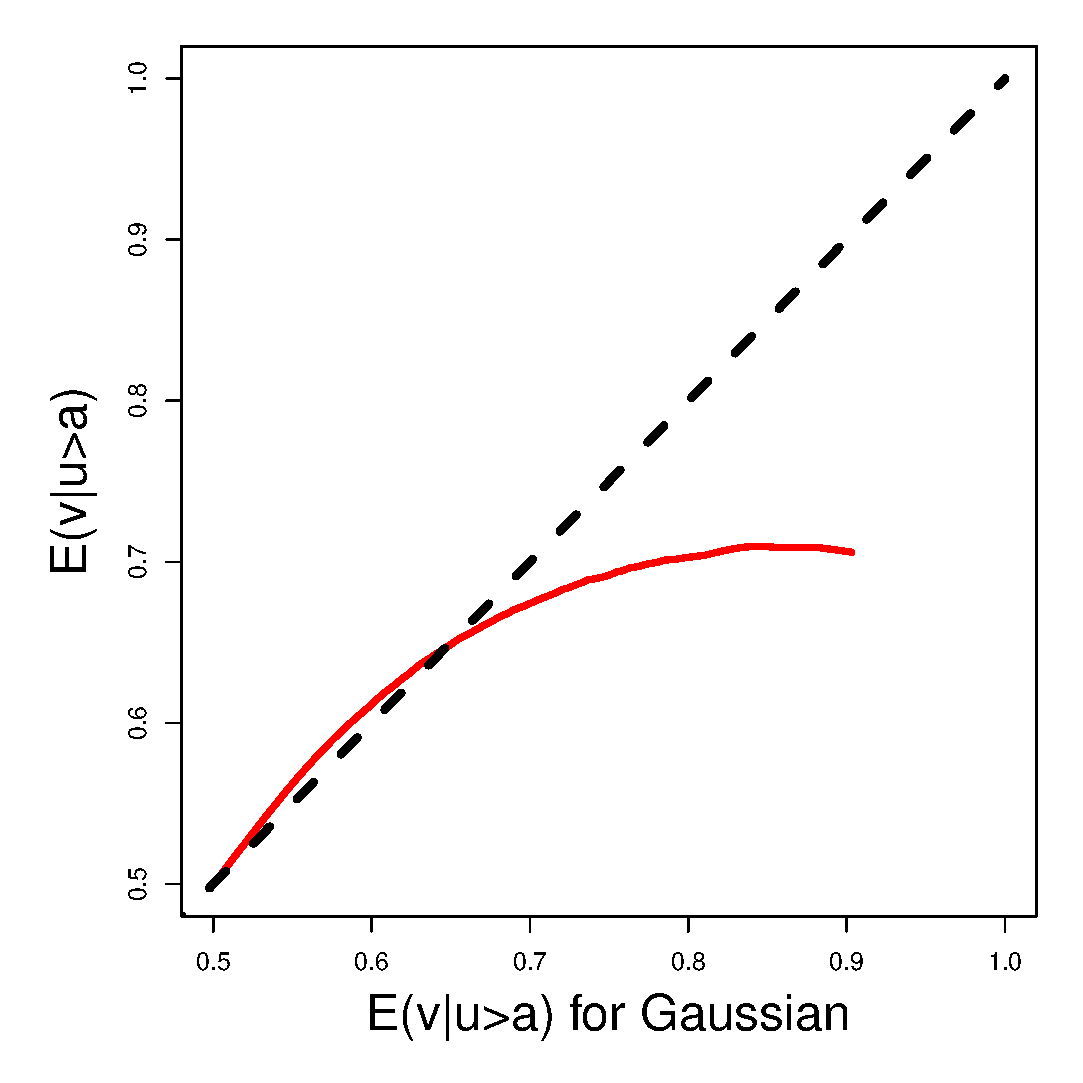
\includegraphics{claytonvs.eps}} \\
            \resizebox{40mm}{!}{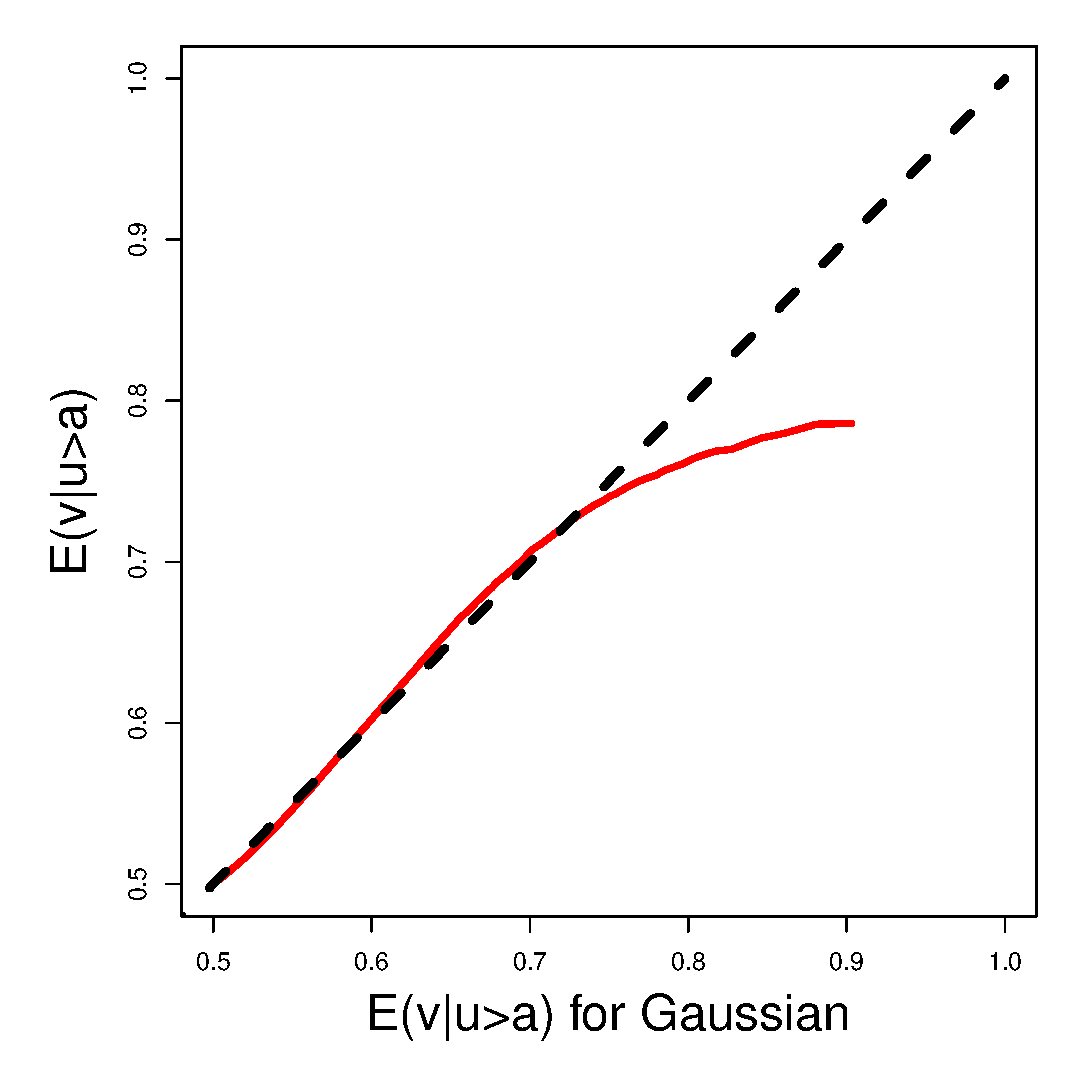
\includegraphics{frankvs.eps}}
            \resizebox{40mm}{!}{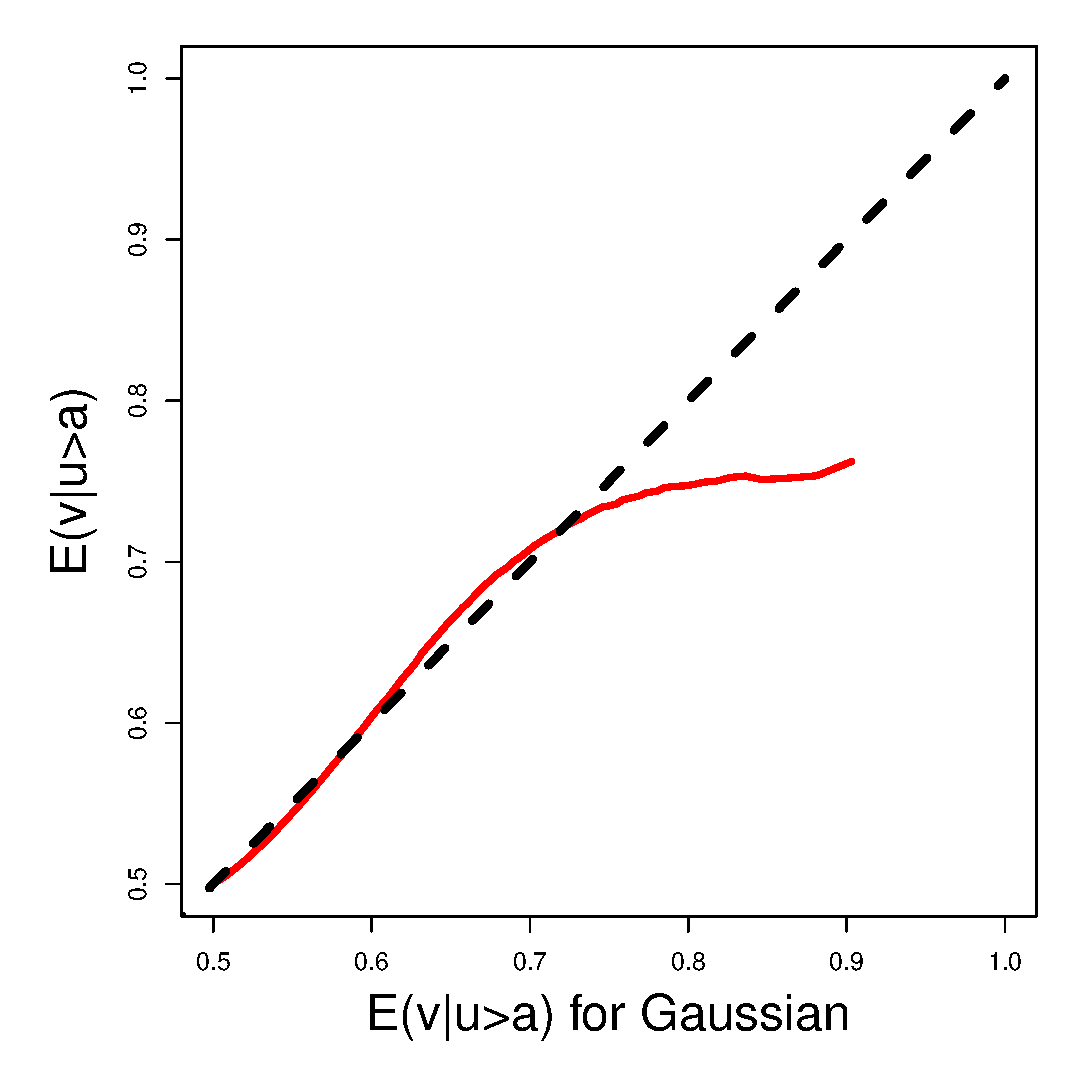
\includegraphics{structural3vs.eps}}
      \resizebox{40mm}{!}{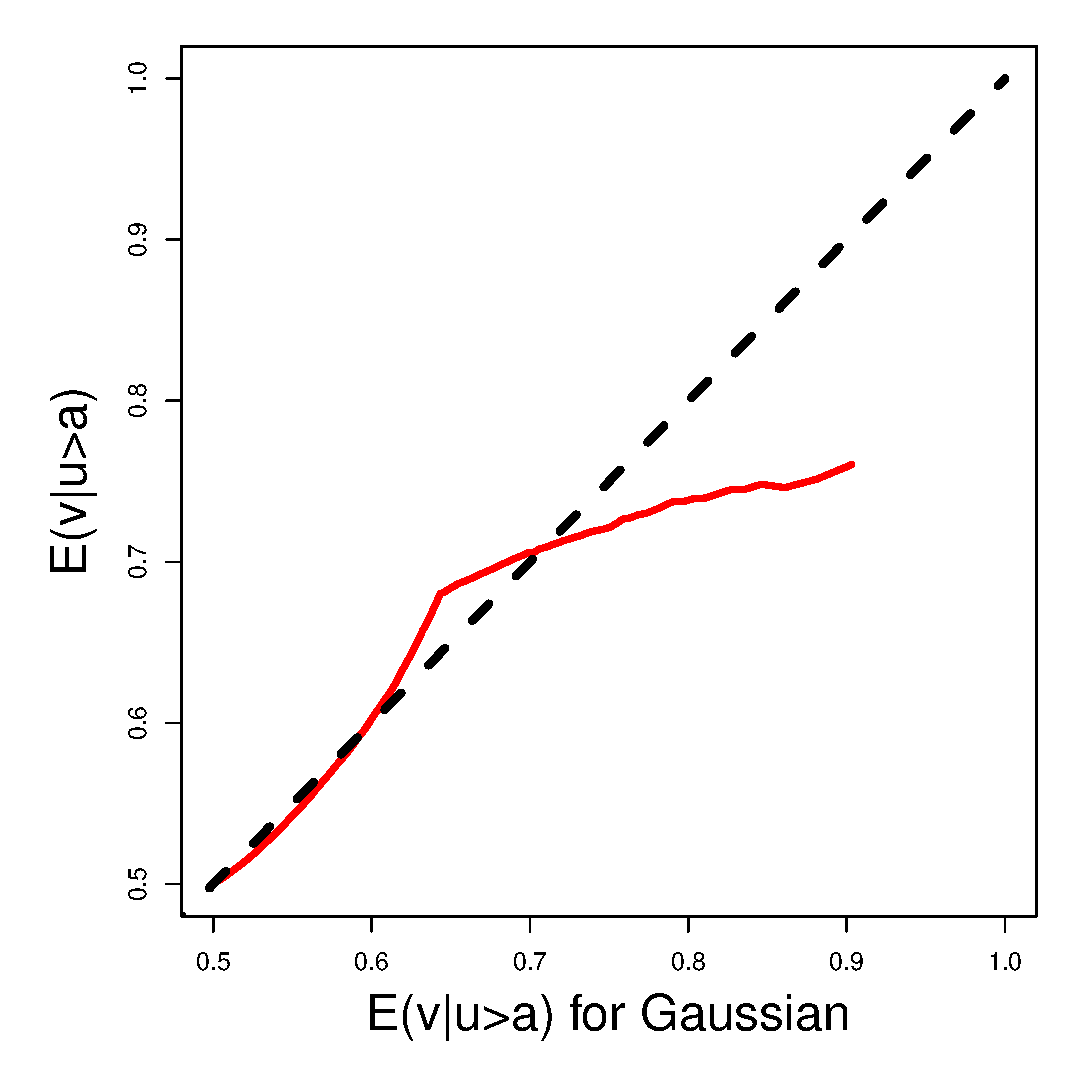
\includegraphics{structural4vs.eps}} \\
    \end{tabular}
    \caption{Plot of upper conditional tail expectations $\E(v|u>\alpha)$ for given copulas against the same for the Gaussian copula.}
    \label{comparison}
  \end{center}
\end{figure}

\fref{fillustration1} expands \fref{fillustration} by graphing layer dependence curves for several parameters of Gaussian, Gumbel, Clayton and Frank copulas. Layer dependence curves summarise essential information (dependence structure) underlying each copula:
\begin{itemize}

\item Gaussian copula: symmetric U-shaped dependence with stronger dependence for larger $\ell$.

\item Gumbel copula: asymmetric U-shaped dependence with stronger dependence for larger $\theta$. Perfect upper tail dependence is always present.

\item Clayton copula: linearly declining dependence with stronger dependence for larger $\theta$. Perfect lower tail dependence is always present.

\item Frank copula: relatively stable dependence with stronger dependence for larger $\theta$.

\end{itemize}
Computing the layer dependence curve is an insightful and important exercise, particularly when the parametric form of a given copula is difficult to interpret, or when the dependence structure underlying an empirical copula is not apparent. Overall dependence measures such as  $\rho_S$ or Kendall's $\tau$ provide information on overall dependence rather than ``local dependence." Section \aref{sliterature} compares layer dependence with existing local dependence measures. It is shown that layer dependence provides a more accurate measure of local dependence. In addition layer dependence possesses coherence properties, further discussed in \sref{scoherence}.

\begin{figure}
  \begin{center}
    \begin{tabular}{cc}
      \resizebox{60mm}{!}{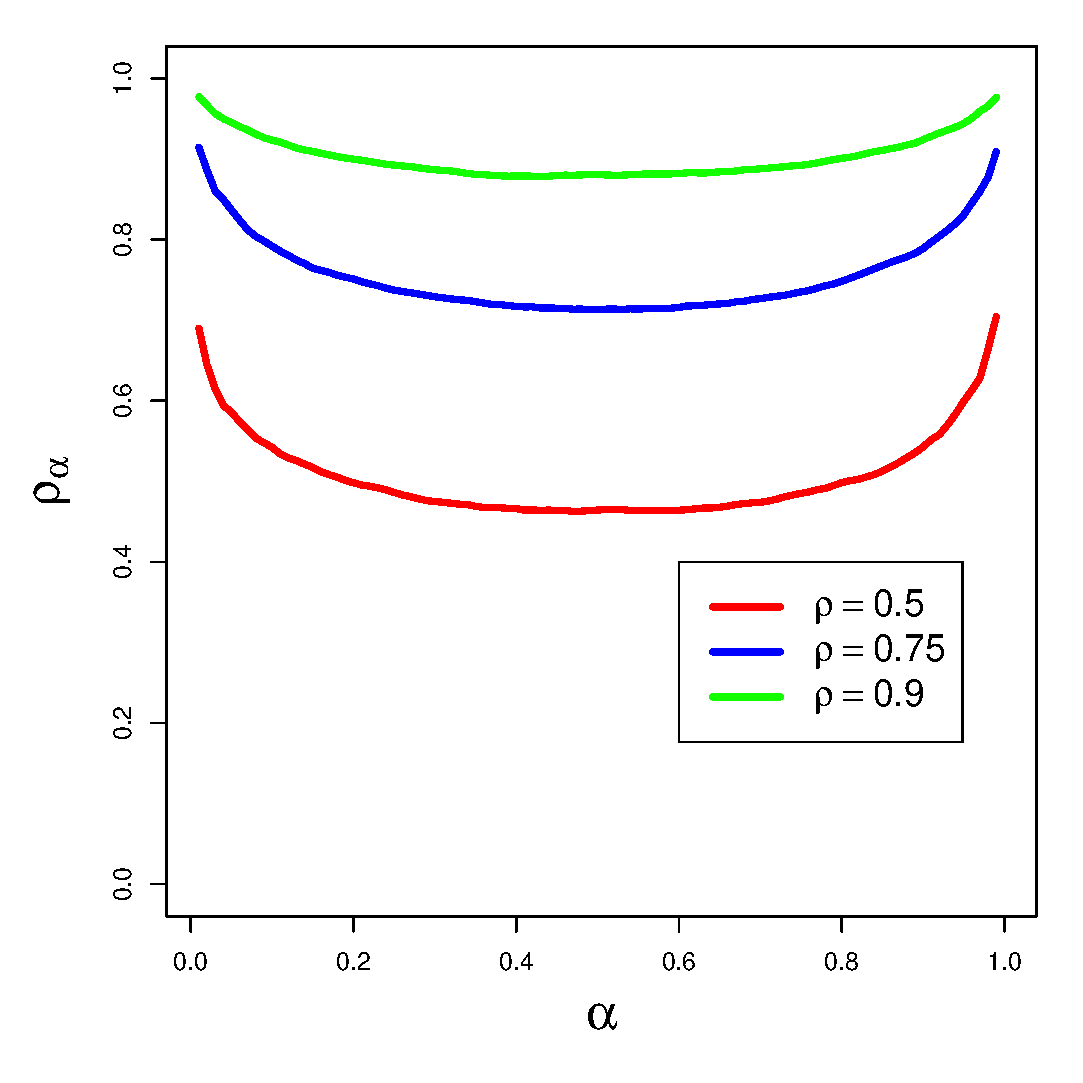
\includegraphics{gaussianmul.eps}}
      \resizebox{60mm}{!}{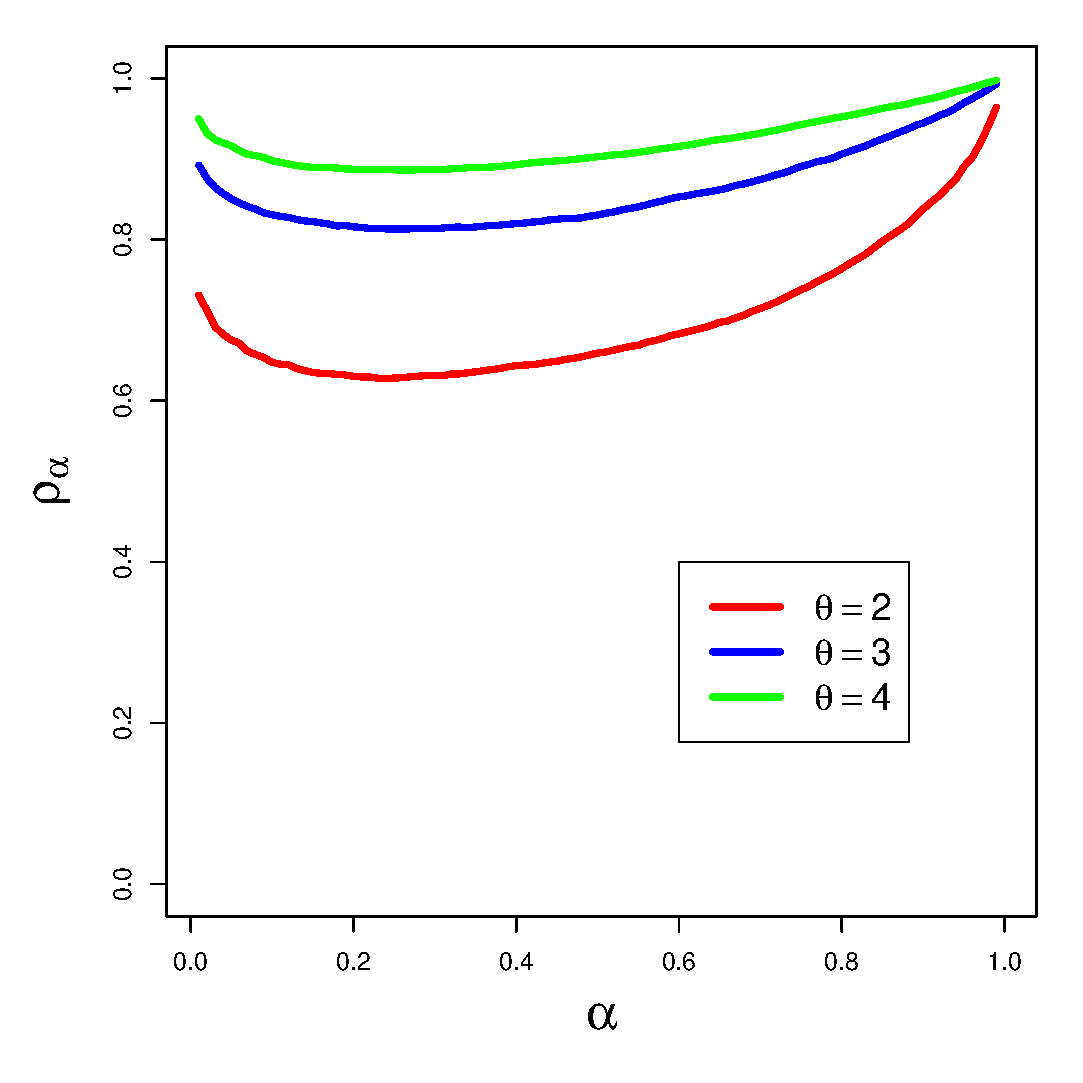
\includegraphics{gumbelmul.eps}} \\
      \resizebox{60mm}{!}{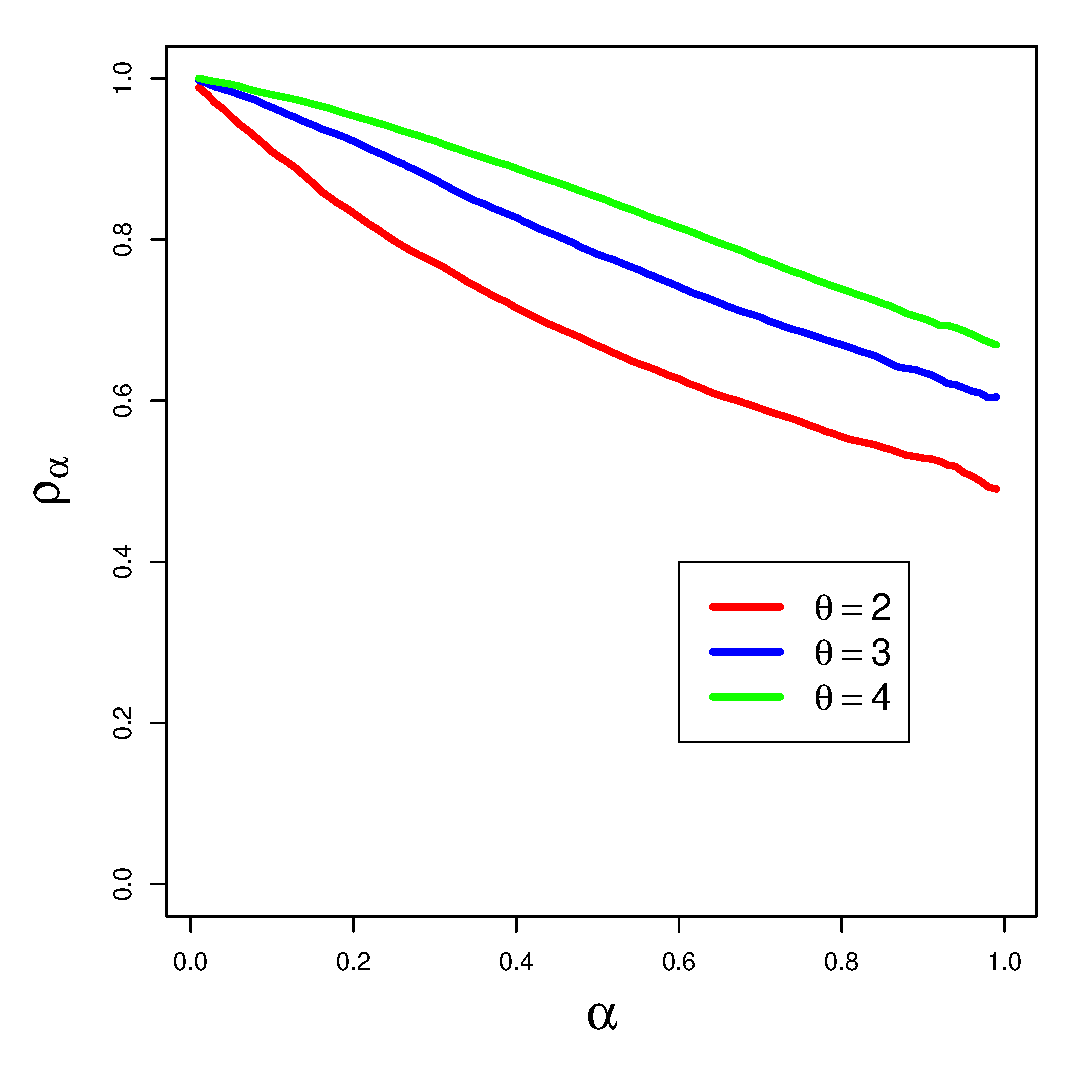
\includegraphics{claytonmul.eps}}
      \resizebox{60mm}{!}{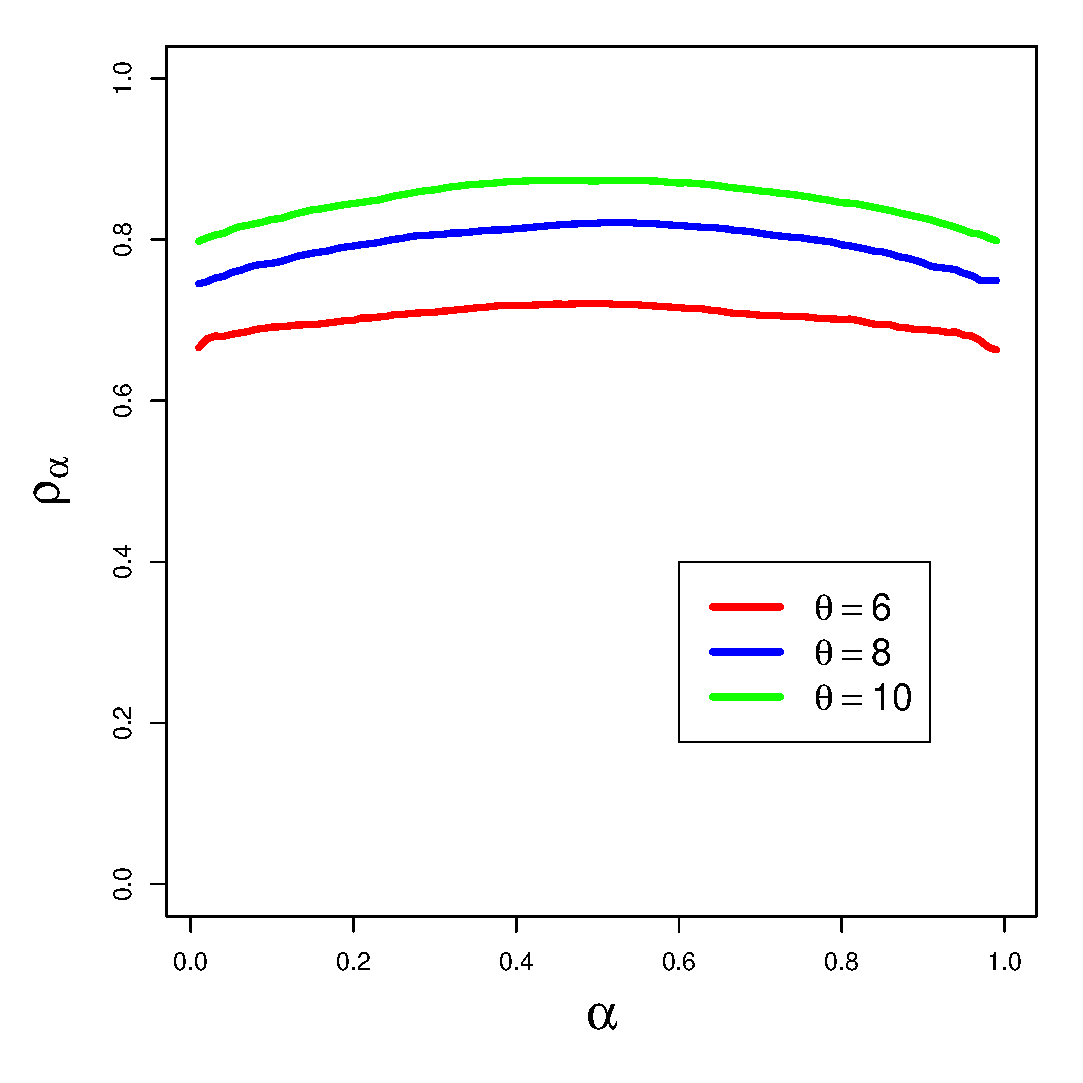
\includegraphics{frankmul.eps}} \\
    \end{tabular}
    \caption{layer dependence curves for various parameters of a Gaussian copula (top left), Gumbel copula (top right), Clayton copula (bottom left) and Frank copula (bottom right). Parameter values are shown in legends.}
    \label{fillustration1}
  \end{center}
\end{figure}





\subsection{``Locality" of layer dependence}

layer dependence $\ell_\alpha$ measures correlation between $u$ in the neighbourhood of $\alpha$ and $v$. This ``locality" property is not apparent from the definition of $\ell_\alpha$. The following is a proof. Define $\ell_{[a,b]}$ as the weighted average
$$
\ell_{[a,b]} \equiv \frac{\int_a^b \ell_\alpha w_\alpha \de \alpha}{\int_a^b w_\alpha \de\alpha}
=\frac{\cov(v,u_{[a,b]})}{\cov(u,u_{[a,b]})}
\cq u_{[a,b]}\equiv \int_a^b (u>\alpha)\de\alpha \;,
$$
where $w_\alpha=6\alpha(1-\alpha)$ and $u_{[a,b]}$ is the ``$[a,b]$ layer" of $u$. Hence the weighted average $\ell_{[a,b]}$ is the scaled correlation between $[a,b]$ layer of $u$ and $v$. Taking the limit $b\rightarrow a^+$ of $\ell_{[a,b]}$ and setting $a=\alpha$ yields $\ell_\alpha$. Rewriting $u_{[a,b]}$ yields
$$
u_{[a,b]}=(u>a)\int_a^{\min(u,b)} \de \alpha = (u>a)\left\{\min(u,b)-a \right\} \;.
$$
Hence the $[a,b]$ layer of $u$ is constant and equal to $0$ when $u\leq a$ and $b-a$ when $u>a$. When $a<u\leq b$, $u_{[a,b]}=u-a$ implying the $[a,b]$ layer of $u$ moves in line with $u$. Therefore the weighted average $\ell_{[a,b]}$ measures correlation between movements of $u$ in the interval $[a,b]$ and $v$. Taking the limit $b\rightarrow a^+$ implies $\ell_\alpha$ measures correlation between $u$ in the neighbourhood of $\alpha$ and $v$. Hence layer dependence measures ``local" dependence.


\subsection{Connection to first-order conditional expectations}

layer dependence in \eref{definition} transforms first order conditional tail expectations into measures of local dependence between $u$ and $v$. Suppose the regression curve of $v$ on $u$, or $\E(v|u=t)$ for all $0\leq t\leq 1$, is given. Then $\alpha$-layer dependence is the integral
$$
\ell_\alpha = 2\left\{\frac{1}{1-\alpha}\int_\alpha^1 \E(v|u=t) \de t - \frac{1}{\alpha}\int_0^\alpha \E(v|u=t) \de t \right\} \;.
$$
Given $\alpha$-layer dependence yields first order conditional expectations:
$$
\E(v|u>\alpha)=\ell_\alpha \E(u|u>\alpha) + 0.5(1-\ell_\alpha)  \;,
$$
$$
\E(v|u=\alpha)=\alpha\ell_\alpha +0.5(1-\ell_\alpha)-0.5\alpha(1-\alpha)\ell'_\alpha \;.
$$
Hence first order conditional expectations are a weighted average of corresponding expectations assuming comonotonicity and independence, with weights $\ell_\alpha$ and $1-\ell_\alpha$, respectively. The conditional expectation $\E(v|u=\alpha)$ requires an additional adjustment term $0.5\alpha(1-\alpha)\ell'_\alpha$ based on the derivative $\ell'_\alpha$.


\end{comment}






\section{Links to the literature}\label{sliterature}





\subsection{Tail dependence}


Tail dependence models dependence at percentiles $0$ and $1$. Perfect tail dependence occurs when catastrophic events such as  bank failure or  market crash manifests in both  series.  Layer dependence models perfect tail dependence by assuming both variables  simultaneously attain minimum or maximum.  Coefficients of tail dependence discussed in  \cite{joe1997multivariate} yield an identical interpretation.


 \cite{joe1997multivariate} defines coefficients of lower and upper tail dependence in terms of the extreme tail probabilities
 $$
\lim_{\alpha\rightarrow 0} \E\{(v\leq \alpha) |u\leq \alpha\} \cq
\lim_{\alpha\rightarrow 1} \E\{(v>\alpha )|u>\alpha\} \;.
$$
Coefficient values of one indicate perfect positive tail dependence, and occur if and only if $u$ and $v$ converge simultaneously to zero (lower tail) or one (upper tail). Negative tail dependence definitions replace $(v\leq \alpha)$ and $(v>\alpha)$ in the above expressions by $(v>1-\alpha)$ and $(v\leq 1-\alpha)$, respectively.


Layer dependence provides a consistent view of perfect tail dependence as \cite{joe1997multivariate}. For the upper tail, from \eref{gapexp}, $\ell_1=2\E(v|u=1)-1$. Hence $\ell_1=1$ if and only if $\E(v|u=1)=1$, that is $\ell_1=1$ if and only if $u=1$ implies $v=1$.   Similarly $\ell_1=-1$ if and only if $u=1$ implies $v=0$. Similar remarks apply to the lower tail:   $\ell_0=1$ if and only if $u=0$ implies $v=0$ while $\ell_0=-1$ if and only if $u=0$ implies $v=1$. Hence perfect tail dependence implies variables simultaneously achieve their extreme values.


\subsection{Tail concentration}

Tail concentration \citep{venter2002tails} is a local dependence measure formed by combining lower and upper conditional tail probabilities at $\alpha$:
$$
\tau_\alpha \equiv (\alpha\leq 0.5) \p(v\leq \alpha|u\leq \alpha) + (\alpha>0.5)\p(v>\alpha|u>\alpha) \;.
$$
Higher tail concentration $\tau_\alpha$ implies $u$ and $v$ are more likely to fall in the same lower tail ($\alpha\leq 0.5$) or upper tail ($\alpha>0.5$). Rewrite tail concentration in terms of the copula $C$ of $(u,v)$:
$$
\tau_\alpha = (\alpha\leq 0.5)\frac{C(\alpha,\alpha)}{\alpha}+(\alpha>0.5)\frac{1-2\alpha+C(\alpha,\alpha)}{1-\alpha} \;.
$$
Standardising tail concentration yields the opposite of the discordance component $\gamma_\alpha$ forming layer dependence in \eref{decomposition}:
$$
\tau_\alpha^* \equiv \frac{\tau_\alpha - \{\alpha(\alpha\leq 0.5)+(1-\alpha)(\alpha>0.5)\}}{1-\{\alpha(\alpha\leq 0.5)+(1-\alpha)(\alpha>0.5)\}}
=\frac{C(\alpha,\alpha)-\alpha^2}{\alpha(1-\alpha)} = -\gamma_\alpha \;,
$$
implying $\ell_\alpha=1-2\delta_\alpha(1-\tau_\alpha^*)$ where $\delta_\alpha$, as defined in section \aref{sdecompose}, is the average dispersion between points $(u,v)$ discordant at $\alpha$. Standardisation subtracts the value under independence: $\tau_\alpha=\alpha(\alpha\leq 0.5)+(1-\alpha)(\alpha>0.5)$, and divides the result by the same where $u$ and $v$ are comonotonic: $\tau_\alpha=1$.

Therefore layer dependence refines tail concentration by including additional information on  average dispersion between discordant points.

\section{Further properties of layer dependence}\label{sproperties}

\subsection{Layer dependence does not uniquely characterise a copula}

Layer dependence curves $\ell_\alpha$ over $0\le\alpha\le 1$ do not uniquely characterise the copula $C$.  For example suppose $v=u$ and $v=1-u$ with equal probability, implying $\E(v|u\leq \alpha)=\E(v|u>\alpha)=0.5$ for all $\alpha$. Then $\ell_\alpha=0$, from \eref{gapexp}. The copula is $C(u,v)=0.5\{\min(u,v)+\max(u+v-1,0)\}$. The same $\ell_\alpha$ results if $u$ and $v$ are independent: $C(u,v)=uv$.

Non-uniqueness arises as layer dependence only captures first-order conditional tail expectations, based on \eref{gapexp}.

\begin{comment}

\subsection{Non-exchangeability}

layer dependence retains coherence and dependence-measuring properties when the joint distribution of $(u,v)$ is non-exchangeable. However the calculation of layer dependence differs according to the conditioning variable:
$$
2\left\{\E(v|u>\alpha)-\E(v|u\leq \alpha)\right\} \neq
2\left\{\E(u|v>\alpha)-\E(u|v\leq \alpha)\right\} \;.
$$
The left expression measures local dependence with respect to $u$. The right expression measures local dependence with respect to $v$, and is not necessarily equal to the left. A similar concept applies in regression, where the regression coefficient depends on the assignment of explanatory and dependent variables.

\end{comment}




\subsection{Layer dependence under non-exchangeable copula}

If $u$ and $v$ are exchangeable, layer dependence in \eref{definition} is invariant when $u$ and $v$ are switched. Archimedean copulas \citep{mcneil2005qrm} are exchangeable. If exchangeability fails then layer dependence differs when layers of $v$ instead of $u$ are applied, that is dependence between $v$ and $\alpha$--layer of $u$ differs from dependence between $u$ and $\alpha$--layer of $v$. An analogous property applies to least squares regression: regressing $v$ on $u$ is the same as  regressing $u$ on $v$, if the joint distribution is  exchangeable.  This paper assumes exchangeability unless stated otherwise.




\subsection{Layer dependence preserves convex combination}

Suppose $(u,v)$ and $(u^*,v^*)$ are both bivariate uniform with layer dependence $\ell_\alpha$ and $\ell_\alpha^*$, respectively. Then  $\pi\ell_\alpha+(1-\pi)\ell_\alpha^*$ is the layer dependence of  $x(u,v)+(1-x)(u^*,v^*)$ where $x\sim B(\pi)$.  The proof  is straightforward using \eref{gapexp}.  This result generalises to multiple and continuous convex combinations of a vector of bivariate uniform random variables.



\section{Other expressions for layer dependence}\label{sotherexp}


\subsection{One-sided conditional tail expectations}


Since $\E(v)=\alpha\E(v|u\leq \alpha)+(1-\alpha)\E(v|u>\alpha)$ it is straightforward to show
$$
\ell_\alpha = \frac{\E(v|u> \alpha)-\E(v)}{\E(u|u> \alpha)-\E(u)} = \frac{\E(v|u\leq \alpha)-\E(v)}{\E(u|u\leq \alpha)-\E(u)} \;,
$$
the gap between upper or lower conditional tail expectations of $v$ and the unconditional expectation. As before denominators are scaling factors ensuring $\ell_\alpha=1$ if $u$ and $v$ are comonotonic and $-1$ if countermonotonic.

\begin{comment}
Rewriting conditional tail expectations in \eref{gapexp} in terms of ``pointwise" conditional expectations yields
$$
\ell_\alpha = 2\left\{\frac{1}{1-\alpha}\int_\alpha^1 \E(v|u=t) \de t - \frac{1}{\alpha}\int_0^\alpha \E(v|u=t) \de t \right\} \;,
$$
hence $\alpha$-layer dependence is the difference between average points on the regression curve of $v$ on $u$ over $u>\alpha$ and $u\leq\alpha$.
\end{comment}


\subsection{Copula integration}

Note $\cov\{(u>\alpha),(v>\beta)\}=C(\alpha,\beta)-\alpha\beta$ and apply \eref{decompose} to $v$, to derive
$$
\ell_\alpha = \frac{\int_0^1 \cov\{(u>\alpha),(v>\beta)\} \de\beta }{\alpha(1-\alpha)/2}
= \frac{2 \int_0^1 C(\alpha,\beta) \de \beta- \alpha}{\alpha(1-\alpha)} = \frac{2 \int_0^1 C(\beta|\alpha) \de \beta- 1}{1-\alpha}\;,
$$
where $C(\beta|\alpha)=\p(v\le\beta|u\le\alpha)$ is the conditional copula. Thus $\ell_\alpha$ integrates copulas and conditional copulas to reduce their dimension from two and one, and scales the result to ensure it lies between $\pm 1$.

With Archimedean copulas \citep{mcneil2005qrm} $C(\alpha,\beta) =\psi^-\left\{\psi(\alpha)+\psi(\beta)\right\}$ where $\psi$ is the generator function and $\psi^-$ its inverse. In this case closed form expressions for the integrals and hence $\ell_\alpha$ or $\E(v|u>\alpha)$  do not exist. This  argues against the use of Archimedean copulas.



\section{Simulating a copula given layer dependence}\label{smodeling}

The following are two approaches to simulate a copula given layer dependence $\ell_\alpha$ for all $0\leq\alpha\leq 1$. The copula is not unique to $\ell_\alpha$ since $\ell_\alpha$, from \eref{gapexp}, relates to first order conditional expectations rather than the entire conditional distribution associated with the copula.


\subsection{Factor model}

The first approach assumes a factor copula model
$$
u=G_{s+\eps}(s+\eps_u) \cq
v=G_{s+\eps}(s+\eps_v) \cq
 s \sim G_s   \cq \eps_u, \eps_v \sim N(0,1) \ ,
$$
where $s$, $\eps_u$ and $\eps_v$ are independent. $G_s$ and $G_{s+\eps}$ are distributions of $s$ and $s+\eps_u$, respectively, and $G_{s+\eps}$ depends on $G_s$. Both $u$ and $v$ are uniform and the joint distribution of $(u,v)$ is exchangeable. The common factor $s$ generates and controls layer dependence between $u$ and $v$.

The factor copula model generates positive layer dependence. Negative layer dependence is created by first simulating the corresponding positive layer dependence, and then taking complements of either percentile rank.

To generate a sample of $(u,v)$ from the factor copula model with layer dependence $\ell_\alpha$, $0\le\alpha\le 1$,  choose a large integer $n$  and simulate $\eps_{u,i},\eps_{v,i}\sim N(0,1)$ for $i=1,\ldots,n$.  Initialise $s_i$ by for example setting it equal to a normal sample with standard deviation chosen such that $s_i+\eps_{u,i}$ and $s_i+\eps_{v,i}$ have Spearman's correlation consistent with $\ell_\alpha$. Then repeat:
\begin{enumerate}

\item Compute ``fitted"  $\hat\ell_{j/n}$ between  $(u_i,v_i)$ for $j=1,\ldots,n$, where $u_i$ and $v_i$ are calculated from the percentile ranks of $s_i+\eps_{u,i}$ and $s_i+\eps_{v,i}$, respectively.

\item Keep $s_1$ unchanged and update  $s_2,\ldots,s_n$ according to
$$
s_{i+1}  \leftarrow s_{i}+  \left(\frac{\ell_{i/n}}{\hat \ell_{i/n}}\right)^a(s_{i+1}-s_i)\cq a>0\;,
$$
in turn yielding an updated sample $(u_i,v_i)$.

\item Go to 1 unless $\|\ell_{i/n} -  \hat\ell_{i/n} \|$ is less than some pre-specified small amount.

\end{enumerate}
Step 1 can be simplified by computing $\hat \ell_{j/n}$ over a fewer number of points and then fitting a parametric curve to computed values. The resulting sample $(u_i,v_i)$ for   $i=1,\ldots,n$ once the iteration is complete has  layer dependence $\hat\ell_\alpha\approx\ell_\alpha$.




\subsection{Regression model}

The second approach writes $\tau_\alpha\equiv\E(v|u>\alpha)=(1+\alpha\ell_\alpha)/2$.  Then
$$
\tau'_\alpha \equiv\frac{\de\E(v|u>\alpha)}{\de\alpha}= \frac{\de}{\de \alpha} \frac{\E\left\{v(u>\alpha)\right\}}{1-\alpha}
= \frac{\tau_\alpha-\mu_\alpha}{1-\alpha}\cq \mu_\alpha\equiv \E(v|u=\alpha)\;,
$$
where $\mu_\alpha$ is the regression curve of $v$ on $u$. Hence $\mu_\alpha=\tau_\alpha-(1-\alpha)\tau'_\alpha$
and $\tau_\alpha$ is monotonic if $\mu_\alpha$ is monotonic.

Suppose $\ell_\alpha$ and hence $\tau_\alpha$ is given for $\alpha=i/n$, $i=1,\ldots,n$ with values denoted $\tau_1,\tau_1,\ldots,\tau_{n}$.   Then  $C(u,v)$ with layer dependence $\ell_\alpha$ is simulated using
$$
v_i=F\{F^-(\mu_i)+\sigma\eps_i\}\ ,\ \mu_{i}=\tau_i - (n-i)(\tau_{i}-\tau_{i-1})\ ,\ \eps_i\sim N(0,1)\ ,\  i=1,\ldots,n\ ,
$$
with $\tau_0=1/2$ and $\sigma$ chosen so that Spearman's $\rho$ for the each sample is expected to match $\rho_S$ implied by $\ell_\alpha$ as in \eref{wtdaverage}.  Here $F$ is an appropriate distribution such as the normal or  logit:  $F^-(\mu_i)=\ln\{\mu_i/(1-\mu_i)\}$.  In the logic case setting $\sigma=1$ appears to ensure a match between the theoretical and empirical $\rho_S$.  To enforce the $v_1,\ldots,v_n$ are empirically uniform the final transformation $F$ can be replaced by $\hat\p$, computing  empirical percentiles.



\section{Copula fitting using layer dependence}\label{sfitting}


\subsection{Approach}

This paper proposes a copula fitting approach based on layer dependence:
\begin{itemize}
\item Calculate layer dependence curve with desired granularity from percentile rank data.

\item Smooth calculated layer dependence curve either parametrically or semi-parametrically.

\item Refine layer dependence using expert knowledge, such as existence and layer of tail dependence.

\item Fit a copula to refined layer dependence curve using methods described in section \aref{smodeling}.
\end{itemize}
The layer dependence approach offers two advantages over fitting parametric copulas. Firstly layer dependence reflects the dependence structure exhibited in past data, whereas parametric copulas, with their relatively restricted dependence structures, may not properly fit past data. Secondly, layer dependence accommodates expert knowledge of local dependence, whereas parametric copulas permit limited changes to the dependence structure once a parametric form is selected.


In comparison to empirical copulas, layer dependence is more robust and less affected by data inadequacies. Layer dependence summarises past data into conditional tail means, and a parametric curve is fitted to calculated values. Hence layer dependence captures advantages of parametric and empirical copulas -- the fitted copula utilises a smooth layer dependence curve, and the dependence structure underlying the fitted copula mirrors past data.



\subsection{Illustration using stock market returns}


The following fits a copula to historical NASDAQ and FTSE daily returns using layer dependence. The dependence structure of the fitted copula mirrors past data, in particular overall and tail dependence.

The left panel in \fref{fmarketindex} plots NASDAQ and FTSE daily percentile rank returns from $1991$ and $2013$. Layer dependence calculated at every integer percentile and  $\rho_S$ are shown in the same panel. Spearman's $\rho_S$ is $0.4$, indicating moderate dependence between NASDAQ and FTSE daily returns. Layer dependence increases towards both tails, hence major positive and negative corrections in NASDAQ and FTSE are likely to occur simultaneously. Lastly layer dependence appears to be symmetric about the $50$th percentile.

The right panel in \fref{fmarketindex} graphs layer dependence refined from empirical values displayed in the left panel, and a copula fitted to refined layer dependence using the factor model. Refined layer dependences closely trace empirical values, including the tails. In addition  $\rho_S$ underlying the fitted copula is approximately equal to the empirical value. Lastly the fitted copula is visually close to past data.

The following outlines the approach to obtain refined layer dependence and the corresponding fitted copula. Derive refined layer dependence by fitting a symmetric polynomial to empirical values:
$$
\hat{\ell}_\alpha = a+b(\alpha-0.5)^2+c(\alpha-0.5)^4   \;,
$$
where $a$, $b$ and $c$ are constants. Least squares estimation by varying $a$, $b$ and $c$ yields a refined layer dependence curve
$$
\hat{\ell}_\alpha = 0.36+0.46(\alpha-0.5)^2+1.73(\alpha-0.5)^4 \cq 0\leq\alpha\leq1 \;.
$$


\begin{figure}
  \begin{center}
    \begin{tabular}{cc}
      \resizebox{60mm}{!}{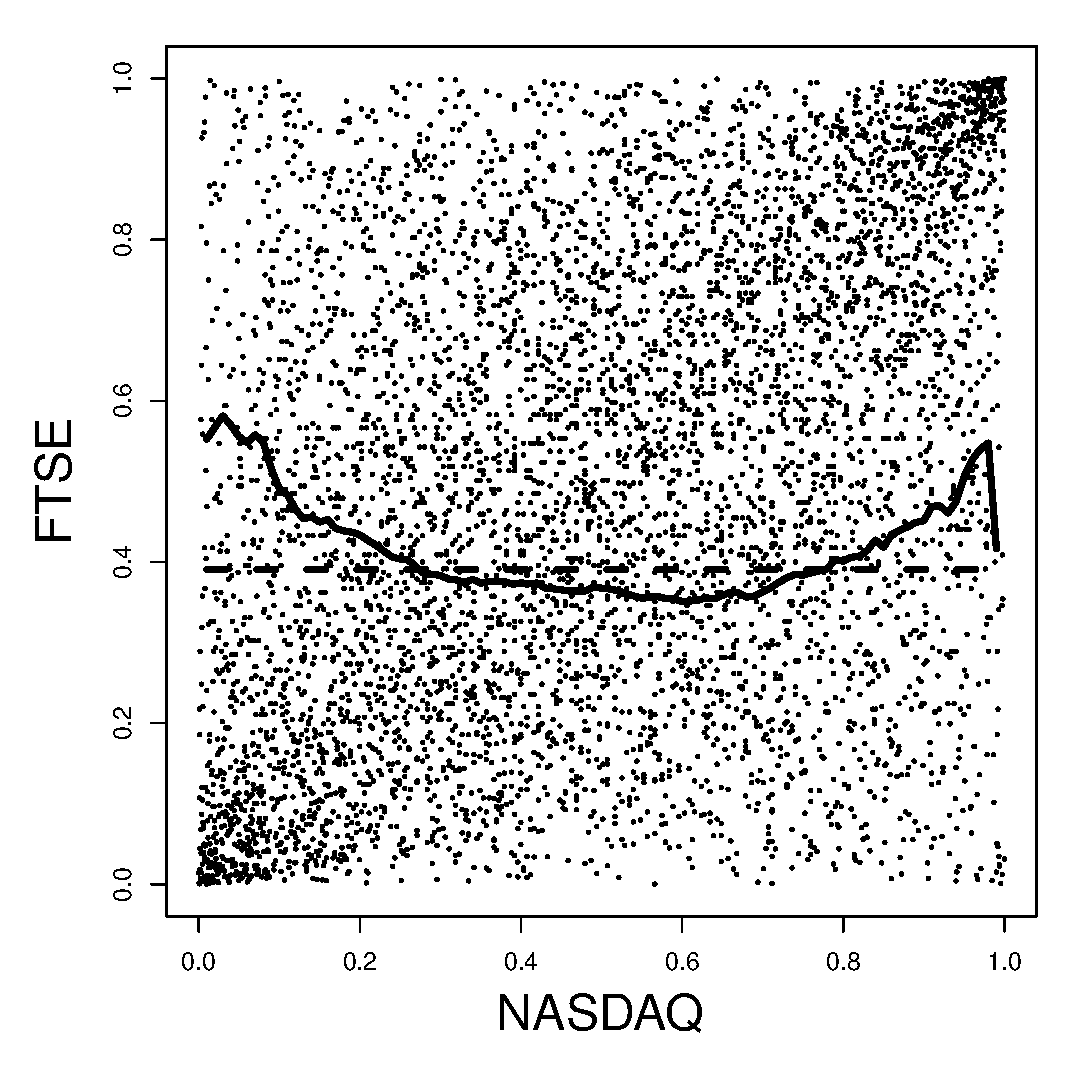
\includegraphics{NASDAQvsFTSE.eps}}
      \resizebox{60mm}{!}{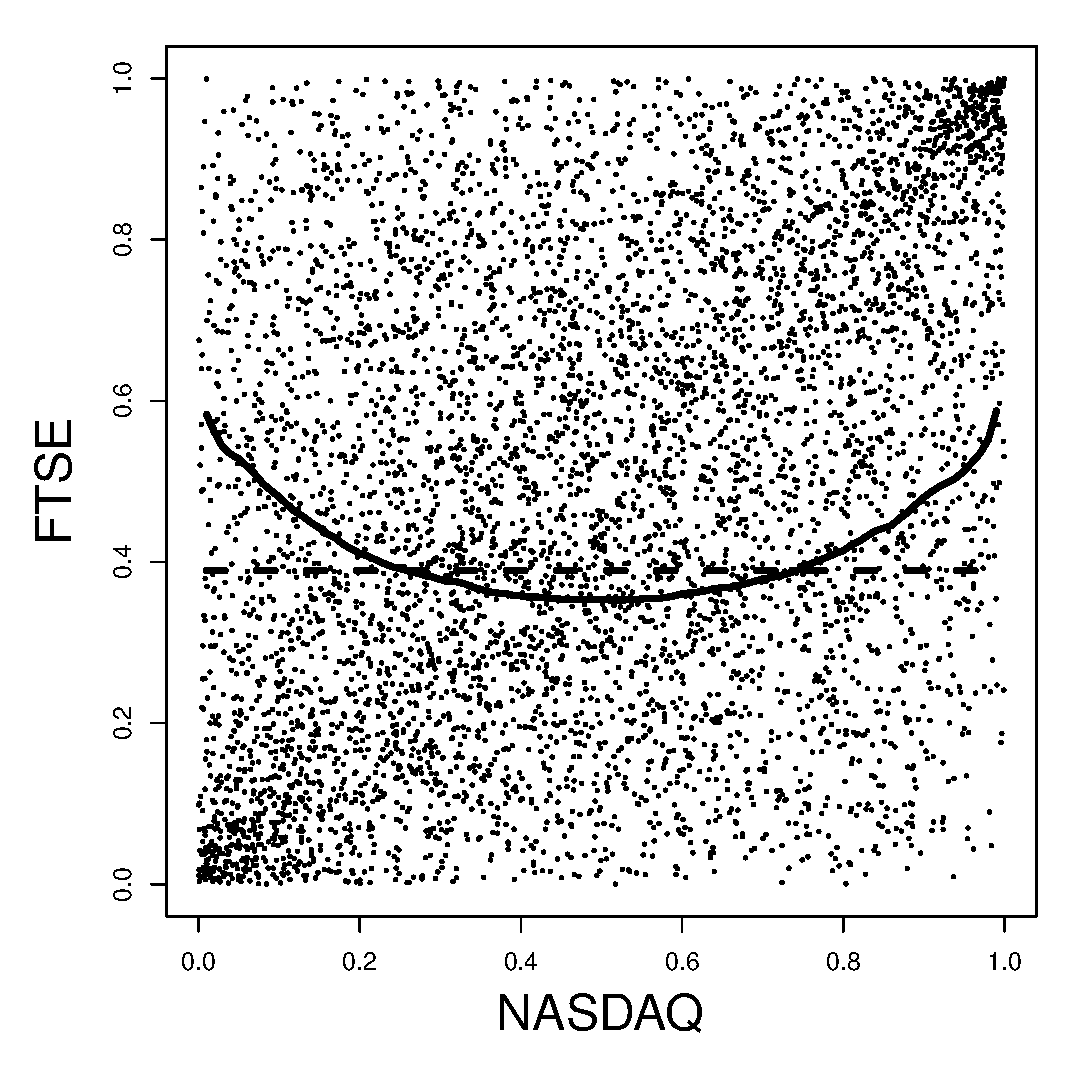
\includegraphics{NASDAQvsFTSE_fitted.eps}} \\
    \end{tabular}
    \caption{The left panel shows daily percentile rank returns from NASDAQ vs FTSE from $1991$ to $2013$, with calculated layer dependence and  $\rho_S$. The right panel shows layer dependence refined from empirical values and a fitted copula.  Spearman's $\rho_S$ underlying the fitted copula is also shown.}
    \label{fmarketindex}
  \end{center}
\end{figure}





\section{Additional applications of layer dependence}\label{sapplication}

The following describes two additional applications of layer dependence. The first is formulate measures of overall rank dependence apart from Spearman's correlation. The second is measuring dependence asymmetry.


\subsection{Alternative measures of overall dependence}


Spearman's correlation is, from \eref{wtdaverage}, an expectation of $\ell_\alpha$ over $\alpha$ using probability density $6\alpha(1-\alpha)$. Alternative rank dependence measures are derived by using a different probability density $w_\alpha$:
$$
\rho_W\equiv  \int_0^1 w_\alpha \ell_\alpha \de \alpha = \int_0^1 w_\alpha \frac{ \cov\{v,(u>\alpha)\}}{\cov\{u,(u>\alpha)\}} \de \alpha=\cov\{W(u),v\} \;,
$$
where
$$
W(u)\equiv 2\int_0^u \frac{w_\alpha}{\alpha(1-\alpha)}\de\alpha \;,
$$
is the weighted cumulative of $w_\alpha$. Hence $\rho_W$  is the covariance between $v$ and a transformation $W(u)$ of $u$.  For Spearman's correlation $\rho_S$, $w_\alpha=6\alpha(1-\alpha)$ and $W(u)\propto u$.

The density $w_\alpha$ specifies ``importance" of dependence at percentile $\alpha$. With Spearman's correlation, $w_\alpha=6\alpha(1-\alpha)$: importance is symmetric and highest at the median, and decreases to zero at both tails. Hence $\rho_S$ emphasizes dependence at moderate percentiles and diminishes dependence in the tails. Alternative densities are described below.

Since $\rho_W$ is a weighted average of $\ell_\alpha$, coherence properties of layer dependence described in section \aref{scoherence} apply to $\rho_W$: bounded by $\pm 1$, constant values of $-1$, $0$ and $1$ under countermonotonicity, independence and comonotonicity, respectively, sign reversal when ranking order switches, and higher values for stronger dependence. Identical properties apply to Spearman's correlation.

The following densities $w_\alpha$ yield alternative rank dependence measures:
\begin{itemize}

\item Suppose dependence over all percentiles are equally important.   Then $w_\alpha$ is the uniform density and
$$
\rho_W =2\cov\left\{v,\log\left(\frac{u}{1-u}\right)\right\}
= \sqrt{\frac{2}{3}}\ \cor\left\{v,\log\left(\frac{u}{1-u}\right)\right\} \;,
$$
\begin{comment}
\int_0^1 \frac{\cov\{v,(u>\alpha)\}}{\cov\{u,(u>\alpha)\}} \de \alpha
=\cov\left[v,\int_0^1 \frac{(u>\alpha)}{\cov\{u,(u>\alpha)\} }\de \alpha\right]
$$
$$
=\cov\left\{v,\int_0^u \frac{1}{0.5\alpha(1-\alpha) }\de \alpha\right\}
\end{comment}
a multiple of correlation between $v$ and the logit of $u$. If tail dependence is pronounced, $\rho_W>\rho_S$ since $\rho_W$ weights tail dependence more heavily compared to $\rho_S$.

\item If $w_\alpha=3\alpha^2$  then dependence at higher percentiles are considered more important. This density is applicable when upper tail dependence exists and has significant impact, for example the simultaneous occurrence of large insurance losses. Then
$$
\rho_W = 6\cov\left\{v,\log\left(\frac{\e^{-u}}{1-u}\right) \right\}
=\sqrt{3} \cor\left\{v,-\log(1-u)\right\}-\frac{\rho_S}{2}\;.
$$
If dependence is higher over percentiles above the median then $\rho_W>\rho_S$.

\item If dependence over percentiles below the median is more important then for example  $w_\alpha=3(1-\alpha)^2$ yielding
$$
\rho_W = 6\cov\left\{v,\log \left( u \e^{-u}\right) \right\}
= \frac{\rho_S}{2}  - \sqrt{3}\cor(v,\log u ) \ .
$$


\item Suppose $w_\alpha$ is derived from $V_\alpha$, the inverse of a marginal distribution function with derivative $V_\alpha'$ such that
$$
w_\alpha = \frac{\cov\{u,(u>\alpha)\}V_\alpha'}{\int_0^1 \cov\{u,(u>\alpha)\}V_\alpha' \de\alpha}
=\frac{\alpha(1-\alpha)V_\alpha'}{\cov(V_u,u)}
=\frac{\alpha(1-\alpha)V_\alpha'}{\cov(x,u)} \;,
$$
where $x=V_u$. This yields the Gini correlation  \citep{schechtman1999proper}
$$
\rho_W=\frac{\cov(V_u,v)}{\cov(V_u,u)} = \frac{\cov\{x,G(y)\}}{\cov\{x,F(x)\}} \;,
$$
where $F\equiv V^-$ and $G$ are distribution functions of $x$ and $y$, respectively.  In this example the density depends on the marginal distribution of $x$. More skewed distributions lead to greater emphasis on upper tail dependence.

\end{itemize}




\subsection{Measuring dependence asymmetry}

Dependence asymmetry is the difference between dependence in upper tail compared to the lower tail. Dependence asymmetry is important for example when modeling the sum of two random variables. Asymmetric dependence, where upper tail dependence is stronger for example, increases the right skewness of the sum since large outcome of both random variables are more likely to occur simultaneously.

Measure dependence asymmetry as $\ell^+-\ell^-$ where
$$
 \ell^+ \equiv \int_z^1 w_\alpha\ell_\alpha \de \alpha
\cq \ell^- = \int_0^{1-z} w_\alpha\ell_\alpha \de \alpha
\cq 0.5\leq z\leq 1\;,
$$
and $w_\alpha$ is a weighting function symmetric about $\alpha=0.5$. Hence dependence in the upper tail is the weighted average of layer dependence over percentiles above $z$, and dependence in the lower tail averages over percentiles below $1-z$. For example the Gaussian or $t$ copulas with symmetric dependence have $\ell^+=\ell^-$. For the Clayton copula, $\ell^->\ell^+$ while $\ell^+>\ell^-$ for the Gumbel copula.

Substituting the expression for $\ell_\alpha$ in \eref{definition} yields
$$
\ell^+
= \cov\left\{ v, \int_z^1 \frac{(u>\alpha)}{0.5\alpha(1-\alpha)} w_\alpha \de \alpha\right\}
=\cov\left\{v,(u>z)\int_z^u \frac{2w_\alpha}{\alpha(1-\alpha)} \de \alpha\right\}
$$
and similarly
$$
\ell^- =  \cov\left\{ v, \int_0^{1-z} \frac{(u>\alpha)}{0.5\alpha(1-\alpha)} w_\alpha \de \alpha\right\}
=\cov\left\{ v, (u\leq 1-z) \int_0^u \frac{2w_\alpha}{\alpha(1-\alpha)} \de \alpha \right\}
$$
$$
+\cov\left\{ v, (u> 1-z)  \right\} \int_0^{1-z}\frac{2w_\alpha}{\alpha(1-\alpha)} \de \alpha \;.
$$




\section{Layer dependence between non--uniform random variables}\label{soriginal}


Consider random variables $x$ and $y$.  Analogous to \eref{definition}, define layer dependence between $x$ and $y$ as the scaled covariance between $y$ and $k$--layer of $x$:
$$
\ell_k^* \equiv \frac{\cov\{y,(x>k)\}}{\cov\{y^*,(x>k)\}} = \frac{\cor\{y,(x>k)\}}{\cor\{y^*,(x>k)\}}\;,
$$
where $k$ lies in the support of $x$, and $y^*$ has identical marginal distribution as $y$ and is comonotonic with $x$. The denominator hence ensures $\ell_k^*=1$ for all $k$ when $x$ and $y$ are comonotonic.

Layer dependence $\ell_k^*$ partially satisfies coherence properties of $\ell_\alpha$ in section \aref{scoherence}. If $x$ and $y$ are independent or comonotonic then $\ell_k^*=0$ and $1$, respectively, for all $k$. If $x$ and $y$ are countermonotonic then write $x=F^-(u)$ and $y=G^-(1-u)$ where $F^-$ and $G^-$ are inverse distribution functions of $x$ and $y$, respectively. Layer dependence in this case is
$$
\ell_k^*  =\frac{\cov\{G^-(1-u),(u>\alpha)\}}{\cov\{G^-(u),(u>\alpha)\}} \leq 0 \cq \alpha=F(k) \;,
$$
reducing to $-1$ if $G^-$ is symmetric: $G^-(1-u)-G(0.5)=G(0.5)-G(u)$. Layer dependence $\ell_k^*$ also preserves correlation order: if $x$ and $y$ increase in correlation order in the sense of \cite{dhaene2009correlation} then $\ell_k^*$ is higher for all $k$, since increase in correlation order translates to increase in covariance values. Layer dependence $\ell_k^*$ is symmetric if the distribution of $y$ is symmetric. Lastly averaging $\ell_k^*$ yields a link to correlation between $x$ and $y$:
$$
\int \frac{\cov\{y^*,(x>k)\}}{\cov(x,y^*)} \ell^*_k \de k = \frac{\cov(x,y)}{\cov(x,y^*)} = \frac{\cor(x,y)}{\cor(x,y^*)}
$$
applying the result in \eref{decompose}.

The four panels \fref{foriginalscale} calculate layer dependence curves between $x$ and $y$ with combinations of symmetric and right skewed beta marginal distributions. A Gumbel copula is assumed. Layer dependence between percentile ranks is included for comparison. Layer dependence retains its overall shape when observed random variables are used instead of percentile ranks.

\begin{figure}
  \begin{center}
    \begin{tabular}{cc}
      \resizebox{60mm}{!}{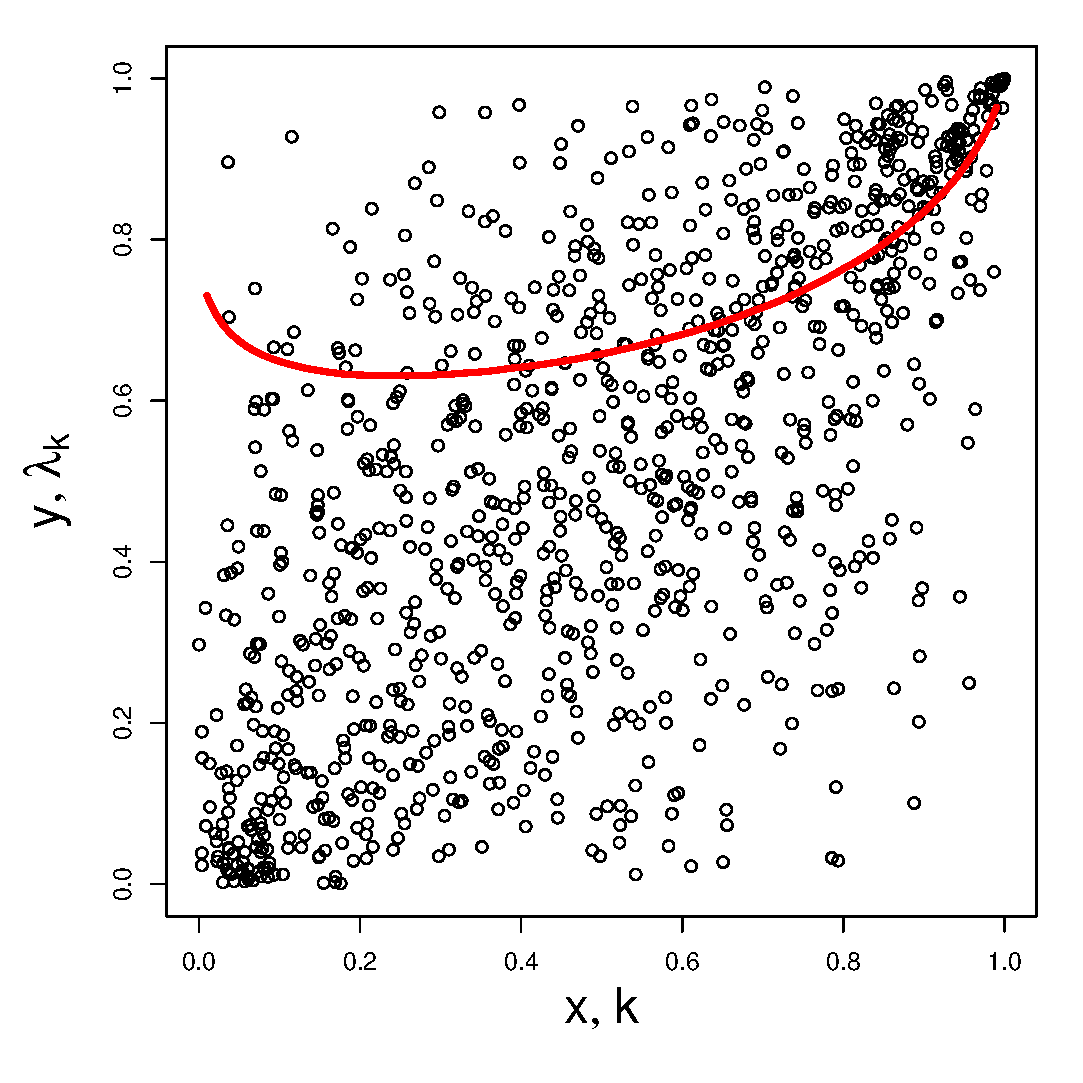
\includegraphics{gumbel0.eps}}
      \resizebox{60mm}{!}{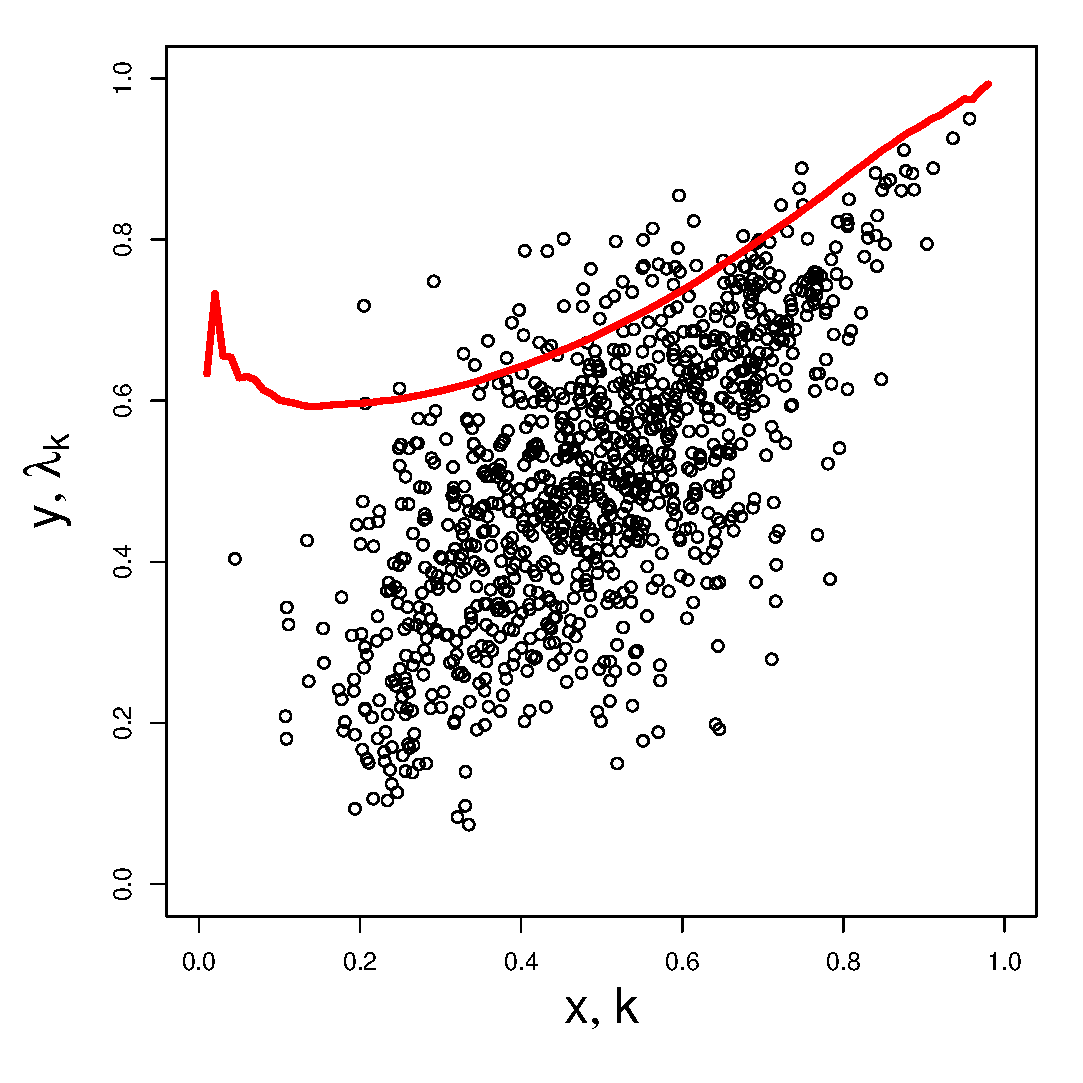
\includegraphics{gumbel1.eps}} \\
      \resizebox{60mm}{!}{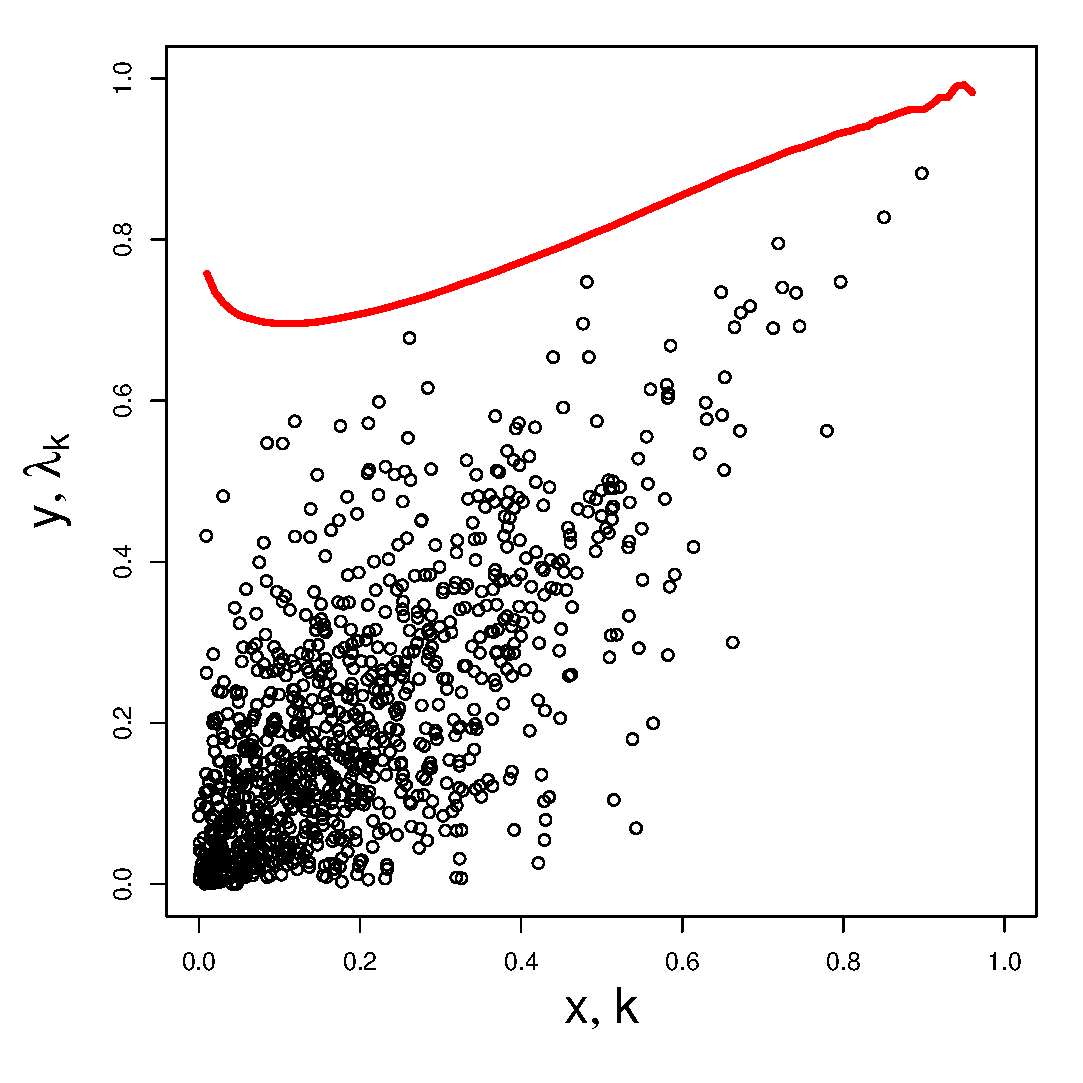
\includegraphics{gumbel2.eps}}
      \resizebox{60mm}{!}{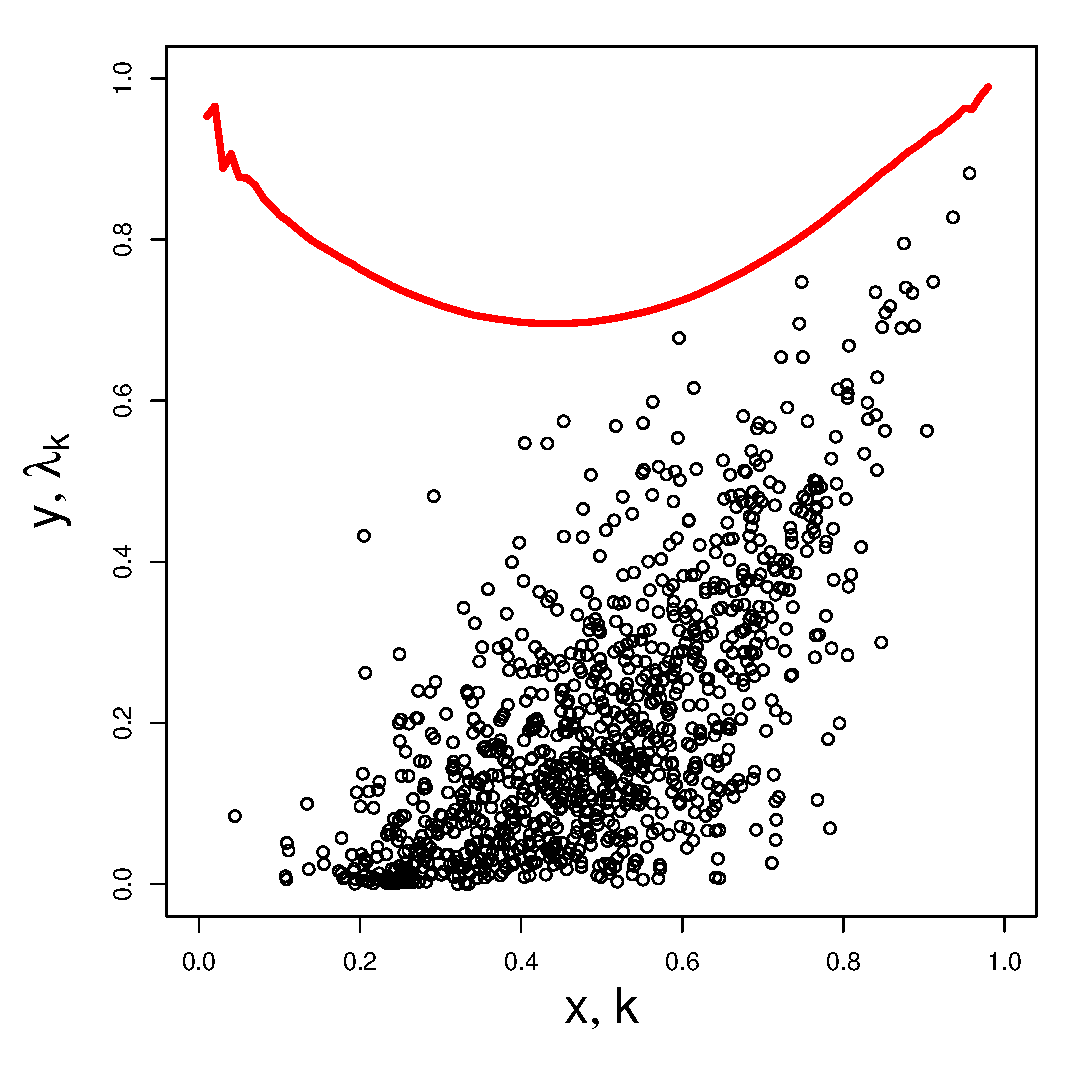
\includegraphics{gumbel3.eps}} \\
    \end{tabular}
    \caption{layer dependence curves between $x$ and $y$ (red line) for a Gumbel copula. The top left panel assumes uniform $x$ and $y$, yielding original layer dependence. The top right panel assumes symmetric $x$ and $y$. The bottom left panel assumes right skewed $x$ and $y$. The bottom right panel assumes symmetric $x$ and right skewed $y$.}
    \label{foriginalscale}
  \end{center}
\end{figure}




\begin{comment}
\subsection{Gap between conditional tail expectations}

Manipulating layer dependence $\ell_\alpha^*$ yields
$$
\ell_\alpha^* = \frac{\E(y|x>V_\alpha)-\E(y|x\leq V_\alpha)}{\E(y^*|x>V_\alpha)-\E(y^*|x\leq V_\alpha)}
=\frac{\E(y|u>\alpha)-\E(y|u\leq\alpha)}{\E(y^*|u>\alpha)-\E(y^*|u\leq\alpha)} \;,
$$
the gap between upper and lower conditional tail expectations of $y$. A similar expression for original layer dependence $\ell_\alpha$ exists in \eref{gapexp}, where conditional tail expectations of percentile rank $v$ are evaluated instead of $y$.

Using the income-education example in \sref{sintroduction}, the population is again divided into two segments depending on whether education is below or above the $\alpha$-percentile. Average actual income is measured in each segment rather than average income ranking. The calculated gap in average actual income is divided by the maximum gap, or the difference between average actual income above and below the $\alpha$-percentile.


\subsection{Link to Pearson correlation}

Taking the following weighted average of $\ell_\alpha^*$ yields scaled Pearson correlation between $x$ and $y$:
$$
\int_0^1 \ell_\alpha^* \left[\frac{\cov\{y^*,(u>\alpha)\}V_\alpha'}{\cov(y^*,x)} \right] \de \alpha
= \frac{\cov\left\{y, \int_0^1 (u>\alpha)V_\alpha' \de \alpha \right\}}{\cov(y^*,x)} =\frac{\cov(y,V_u)}{\cov(y^*,x)}
$$
$$
= \frac{\cor(y,x)}{\cor(y^*,x)}
\cq \int_0^1 \frac{\cov\{y^*,(u>\alpha)\}V_\alpha'}{\cov(y^*,x)}  \de \alpha= \frac{\cov(y^*,V_u)}{\cov(y^*,x)} = 1 \;,
$$
where weights integrate to one. The denominator $\cor(y^*,x)$ in scaled Pearson correlation ensures unity if $x$ and $y$ are comonotonic. Similarly a weighted average of layer dependence $\ell_\alpha$ over all $\alpha$, using quadratic weights, yields  $\rho_S$ as shown in \eref{wtdaverage}.

\subsection{Relationship between two layer dependences}

layer dependences between original random variables and between their percentile ranks are generated by a common ``dependence generating function"
$$
g_{\alpha,\beta}\equiv \frac{\cov\{(u>\alpha,v>\beta)\}}{\cov\{(u>\alpha,u>\beta)\}}
= \frac{C(\alpha,\beta)-\alpha\beta}{\min(\alpha,\beta)-\alpha\beta}  \cq 0\leq \alpha,\beta\leq 1\;,
$$
where $C$ is the copula underlying $(u,v)$. The dependence generating function $g_{\alpha,\beta}$ measures dependence between $\alpha$-layer of $x$ and $\beta$-layer of $v$. In particular $g_{\alpha,\beta}=1$ for all $\alpha$ and $\beta$ if $u$ and $v$ are perfectly dependent, and $g_{\alpha,\beta}=0$ if $u$ and $v$ are independent. Negative dependence yields negative $g_{\alpha,\beta}$.

Taking a weighted average of $g_{\alpha,\beta}$ over all $\beta$ yields layer dependence, between percentile ranks and between observed random variables. Layer dependence $\ell_\alpha$ is generated by the weighted integral
$$
\ell_\alpha= \int_0^1 w_{\beta,1} g_{\alpha,\beta} \de\beta
\cq w_{\beta,1}=\frac{\min(\alpha,\beta)-\alpha\beta}{\int_0^1 \{\min(\alpha,\beta)-\alpha\beta\}\de\beta}
=\frac{\min(\alpha,\beta)-\alpha\beta}{0.5\alpha(1-\alpha)}
$$
and layer dependence $\ell_\alpha^*$ is generated by a different weighted integral
$$
\ell_\alpha^* = \int_0^1 w_{\beta,2}   g_{\alpha,\beta} \de G^-(\beta)
\cq w_{\beta,2}=\frac{\min(\alpha,\beta)-\alpha\beta}{\int_0^1 \{ \min(\alpha,\beta)-\alpha\beta\}\de G^-(\beta)}
$$
$$
=\frac{\min(\alpha,\beta)-\alpha\beta}{\cov \{G^-(u),(u>\alpha)\}}  \;.
$$
For $\ell_\alpha^*$, weights attached to $g_{\alpha,\beta}$ are proportional to the derivative $(G^-)'$. Hence $g_{\alpha,\beta}$ is weighted more heavily over values of $\beta$ where the derivative $\{G^-(\beta)\}'$ is large, such as in the tail of a right skewed distribution. In comparison weights for layer dependence $\ell_\alpha$ are ``marginal free."

The dependence generating function captures complete dependence information due to its direct relationship with the copula $C$. Correlations $\cor(u,v)$ and $\cor(x,y)$ show completely summarised dependence information. Layer dependences $\ell_\alpha$ and $\ell_\alpha^*$ balances the extremes and shows dependence information on a single dimension.

\end{comment}



\begin{comment}

\section{Comparison with existing local dependence measures}\label{sliterature}

This section compares layer dependence with existing local dependence measures: tail concentration \citep{venter2002tails}, correlation curve \citep{bjerve1993correlation}, and bivariate measures by \cite{bairamov2003new}, \cite{jones1996local} and \cite{holland1987dependence}. Calculations are applied to copulas in \fref{fillustration}. Layer dependence is more reflective of local dependence (dispersion and concordance between points), and satisfies all five coherence properties in \sref{scoherence}. In addition there is a direct relationship between layer dependence and  $\rho_S$ in \eref{wtdaverage}.



\subsection{Tail concentration}

\cite{venter2002tails} defines tail concentration at $0\leq\alpha\leq 1$ by combining lower and upper conditional tail probabilities relative to $\alpha$:
\begin{equation}\label{tailcon}
\tau_\alpha \equiv (\alpha\leq 0.5) \p(v\leq \alpha|u\leq \alpha) + (\alpha>0.5)\p(v>\alpha|u>\alpha) \;.
\end{equation}
Higher tail concentration implies $u$ and $v$ are more likely to fall in the same lower tail ($\alpha\leq 0.5$) or upper tail ($\alpha>0.5$). Tail concentration partially satisfies coherence properties described in \sref{scoherence}, and partially reflects local dependence. Layer dependence refines tail concentration through standardisation and reflecting average dispersion between discordant points. Further discussion of tail concentration is shown below.

Rewrite tail concentration in terms of the copula $C$ of $(u,v)$:
$$
\tau_\alpha = (\alpha\leq 0.5)\frac{C(\alpha,\alpha)}{\alpha}+(\alpha>0.5)\frac{1-2\alpha+C(\alpha,\alpha)}{1-\alpha} \;,
$$
therefore tail concentration depends only on the diagonal section of the copula, and is hence symmetric in $u$ and $v$. Independence implies $\tau_\alpha=\alpha(\alpha\leq 0.5)+(1-\alpha)(\alpha>0.5)$, and comonotonicity and countermonotonicity yield $\tau_\alpha=1$ and $\tau_\alpha=0$, respectively. Hence tail concentration does not satisfy independence and perfect dependence (countermonotonicity) coherence properties. Symmetry is also not satisfied since tail concentration is non-negative. The ordering property is satisfied since tail concentration increases with the copula $C$. Lastly $0\leq\tau_\alpha\leq 1$ since $\tau_\alpha$ is a probability, hence the bounds property holds.

Standardising tail concentration improves its coherence and reflection of local dependence. The latter is demonstrated via an illustration below. Standardisation involves subtracting the value assuming independence, and dividing the result by its maximum value:
$$
\tau_\alpha^* \equiv \frac{\tau_\alpha - \{\alpha(\alpha\leq 0.5)+(1-\alpha)(\alpha>0.5)\}}{1-\{\alpha(\alpha\leq 0.5)+(1-\alpha)(\alpha>0.5)\}}
=\frac{C(\alpha,\alpha)-\alpha^2}{\alpha(1-\alpha)} = \gamma_\alpha \;.
$$
Standardised tail concentration $\tau_\alpha^*=0$ if $u$ and $v$ (independence property), and is negative if $u$ and $v$ are negatively dependent. Standardised tail concentration is also equal to the measure of concordance $\gamma_\alpha$ defined in \eref{concordance}.

From \eref{decomposition}, layer dependence combines standardised tail concentration $\tau_\alpha^*=\gamma_\alpha$ and average dispersion between discordant points $\delta_\alpha$. Hence layer dependence refines tail concentration in two ways:
\begin{itemize}

\item layer dependence includes standardisation to achieve coherence. Standardisation also yields a more accurate reflection of local dependence.

\item layer dependence reflects average dispersion between discordant $u$ and $v$, yielding additional accuracy in local dependence measurement.
\end{itemize}
\fref{fventerillustration} demonstrates the above refinements by comparing tail concentration, its standardised value and layer dependence using identical copulas as \fref{fillustration}. Tail concentration, without standardisation, does not always trace local dependence. For example tail concentration decreases at the upper tail of the Gumbel copula, despite upper tail dependence. Similarly for the Clayton copula. Standardisation corrects these inconsistencies. Layer dependence further refines the calculation by reflecting dispersion between discordant points. For example layer dependence increases to one at the upper tail of the Gumbel copula and lower tail of the Clayton copula, whereas standardised tail concentration does not increase completely to one, despite the presence of tail dependence. In addition standardised tail concentration decreases significantly at both tails of Guassian and Frank copulas although there is no increased dispersion of $(u,v)$ in those areas.
\begin{figure}
  \begin{center}
    \begin{tabular}{cc}
      \resizebox{60mm}{!}{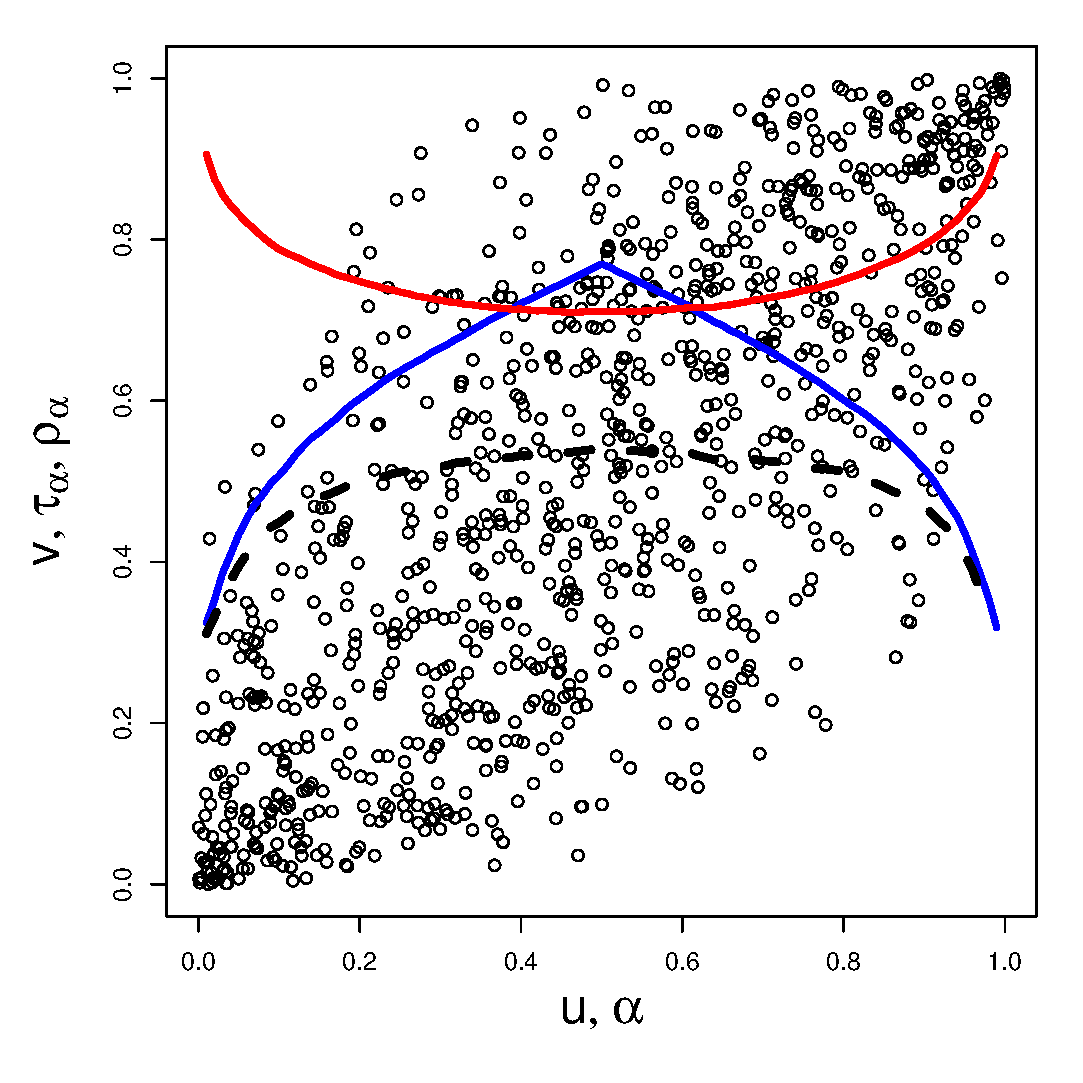
\includegraphics{vnormal.eps}}
      \resizebox{60mm}{!}{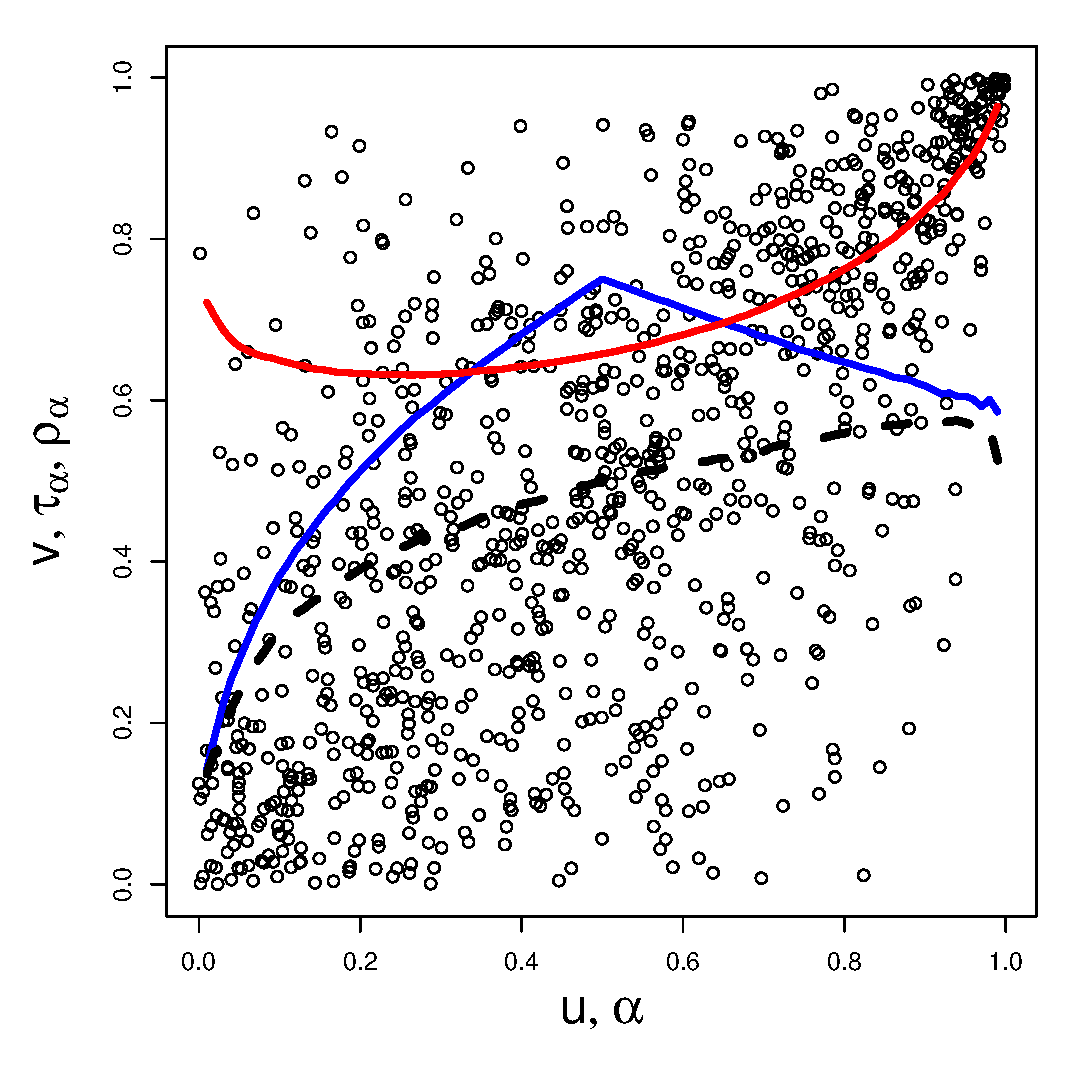
\includegraphics{vgumbel.eps}} \\
      \resizebox{60mm}{!}{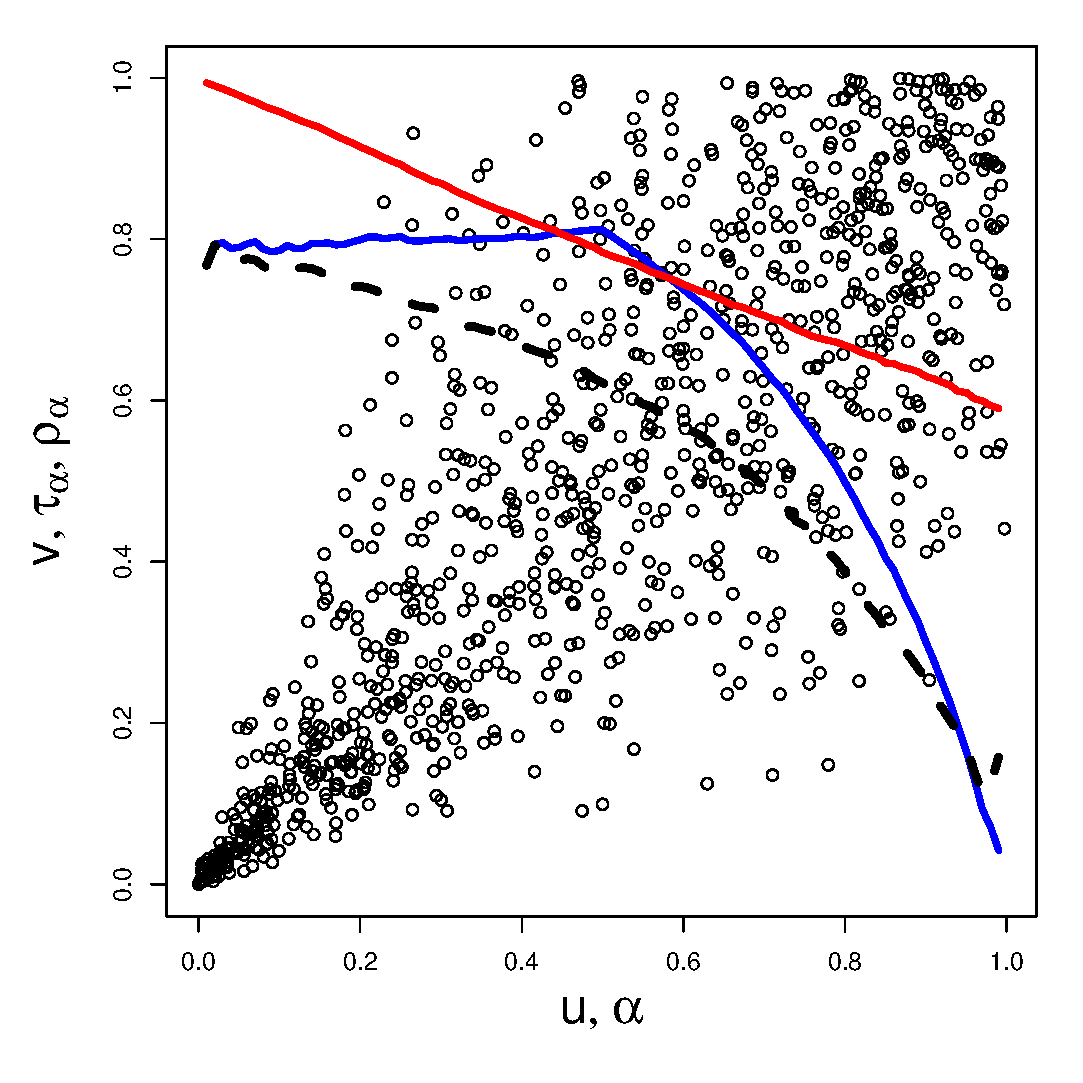
\includegraphics{vclayton.eps}}
      \resizebox{60mm}{!}{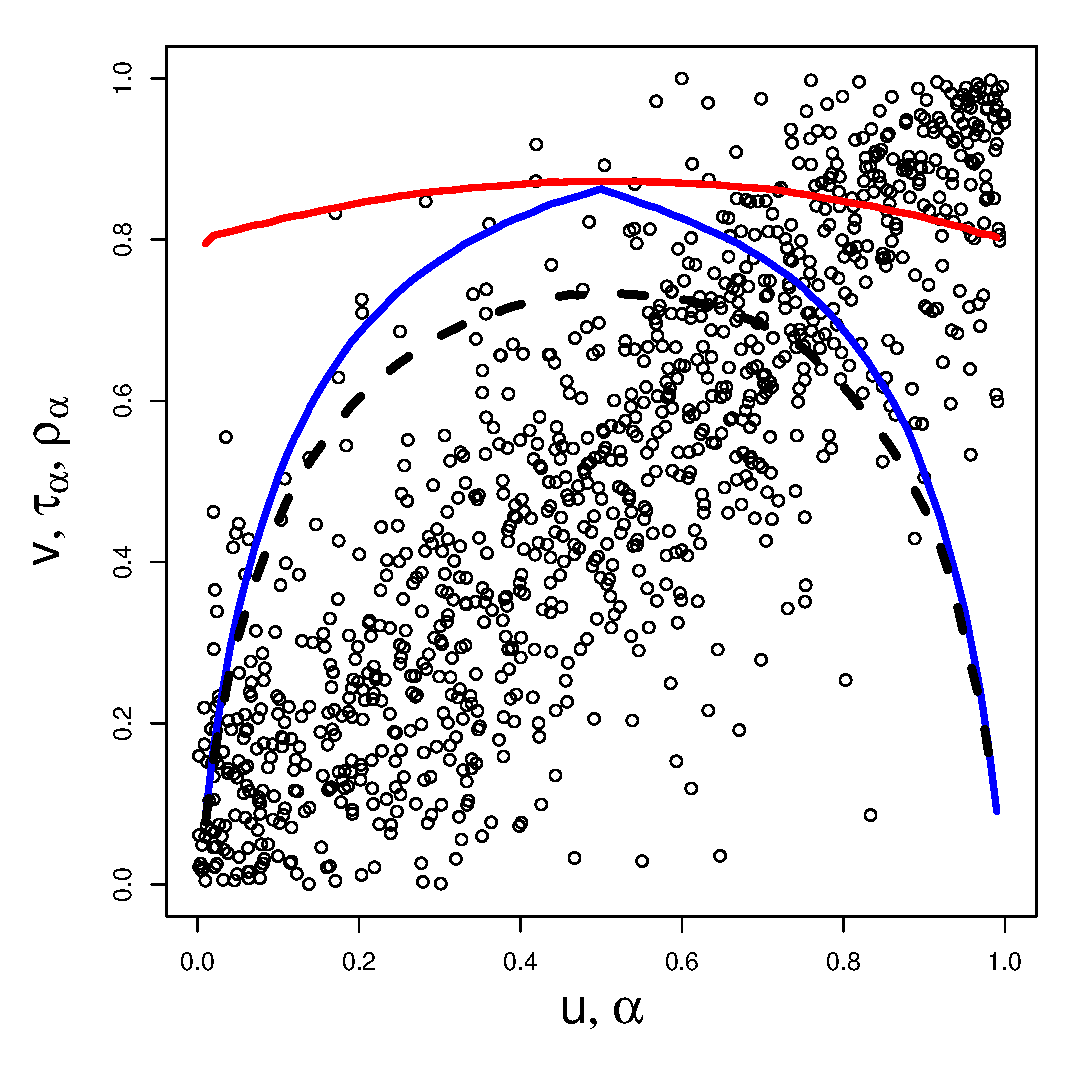
\includegraphics{vfrank.eps}} \\
    \end{tabular}
    \caption{Calculation of tail concentration (blue line) for a Gaussian copula (top left), Gumbel copula (top right), Clayton copula (bottom left) and Frank copula (bottom right). Standardised values (dotted line) and layer dependence (red line) are also shown in each panel.}
    \label{fventerillustration}
  \end{center}
\end{figure}



\subsection{Correlation curve}

\cite{bjerve1993correlation} defines correlation curve based on the conditional distribution of $v$ given $u$. Correlation curve has similar values and coherence properties as layer dependence. However calculated values of correlation curve are volatile due to reliance on a ``pointwise" conditional distribution.

From \cite{bjerve1993correlation}, the correlation curve of $v$ with respect to $u$ at $\alpha$ is defined as
$$
c_\alpha \equiv \frac{\sigma\mu_\alpha'}{\sqrt{(\sigma\mu_\alpha')^2+\sigma_\alpha^2}} = \sign(\mu_\alpha') \times \frac{1}{\sqrt{1+s_\alpha^2}}
\cq 0\leq\alpha\leq 1 \;,
$$
$$
s_\alpha^2\equiv \left(\frac{\sigma_\alpha}{\mu_\alpha'\sigma}\right)^2  \cq \sigma^2\equiv \var(v) \cq \sigma_\alpha^2\equiv \var(v|u=\alpha)
\cq \mu_\alpha\equiv \E(v|u=\alpha) \;.
$$
where $\mu_\alpha$ and $\sigma_\alpha^2$ are the conditional mean and variance of $v$ at $u=\alpha$, respectively, and $\sigma^2=1/12$ is the unconditional variance of $v$. In addition $\mu_\alpha'$ is the derivative of $\mu_\alpha$ with respect $\alpha$. \cite{bjerve1993correlation} also generalises the correlation curve by replacing mean and variance with other location and scale measures such as median and interquartile range, respectively.


The correlation curve $c_\alpha$ at any $\alpha$ is affected by two factors: the derivative $\mu'_\alpha$ and the ratio $\sigma_\alpha^2/\sigma^2$. The former is the sensitivity of the conditional mean of $v$ to changes in $u=\alpha$. Higher sensitivity implies stronger local dependence between $u$ and $v$, increasing $c_\alpha$. The second is the conditional variance of $v$ relative to the unconditional variance. A higher ratio implies values of $v$ conditional on $u=\alpha$ are more variable, hence the conditional mean of $v$ at $u=\alpha$ is a less satisfactory predictor of $v$. The result is lower local dependence and $c_\alpha$.


Correlation curve satisfies similar coherence properties as layer dependence. In particular, for all $\alpha$, $-1\leq c_\alpha\leq 1$ and $c_\alpha=-1$, $0$ and $1$ if $u$ and $v$ are countermonotonic, independent and comonotonic, respectively. Replacing $u$ or $v$ with its complement reverse the sign of $c_\alpha$. In addition $c_\alpha$ increases when $u$ and $v$ are more ``regression dependent.'' \cite{bjerve1993correlation} further discusses properties of correlation curves.


\fref{fcorcurve} graphs correlation curves using identical copulas as \fref{fillustration}. Layer dependence is included as a comparison. Correlation curve varies similarly as layer dependence in all four copulas. However values of correlation curve are volatile, despite a large sample size of $10$ million. In comparison calculations of layer dependence in \fref{fillustration} utilises a $100000$-sample. The volatile correlation curve is due to involvement of conditional means, the derivative, and conditional variances at specific values of $u$.
\begin{figure}
  \begin{center}
    \begin{tabular}{cc}
      \resizebox{60mm}{!}{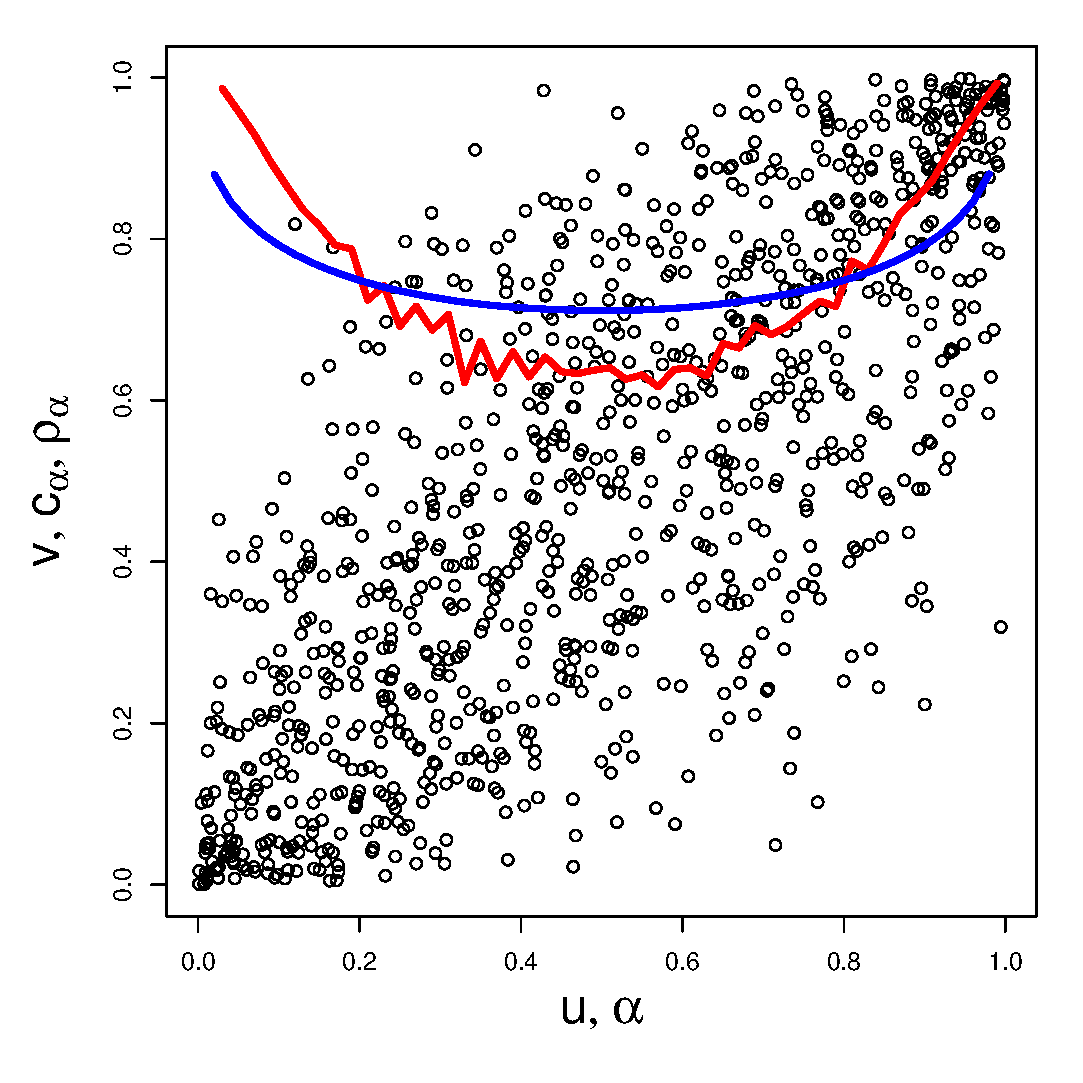
\includegraphics{cnormal.eps}}
      \resizebox{60mm}{!}{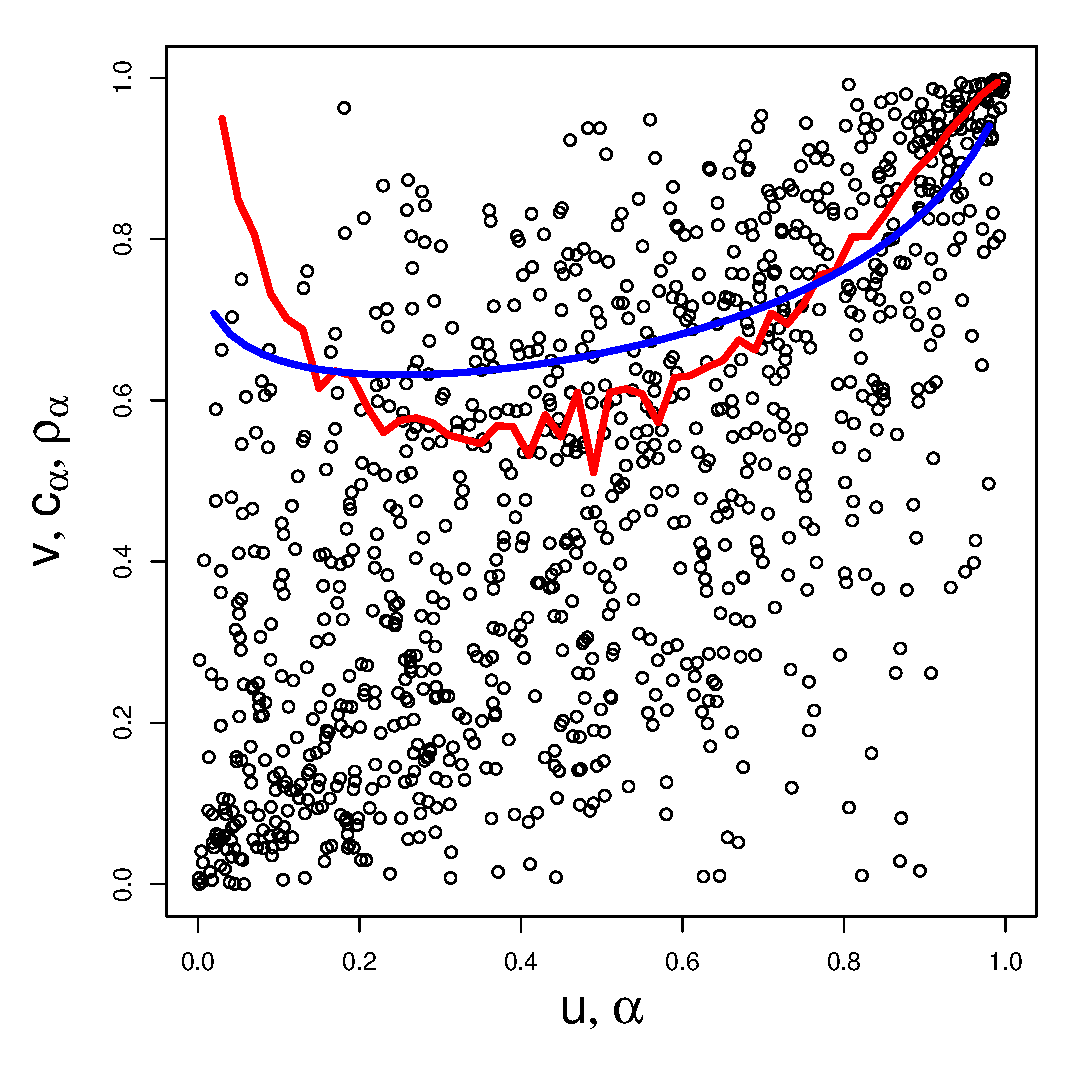
\includegraphics{cgumbel.eps}} \\
      \resizebox{60mm}{!}{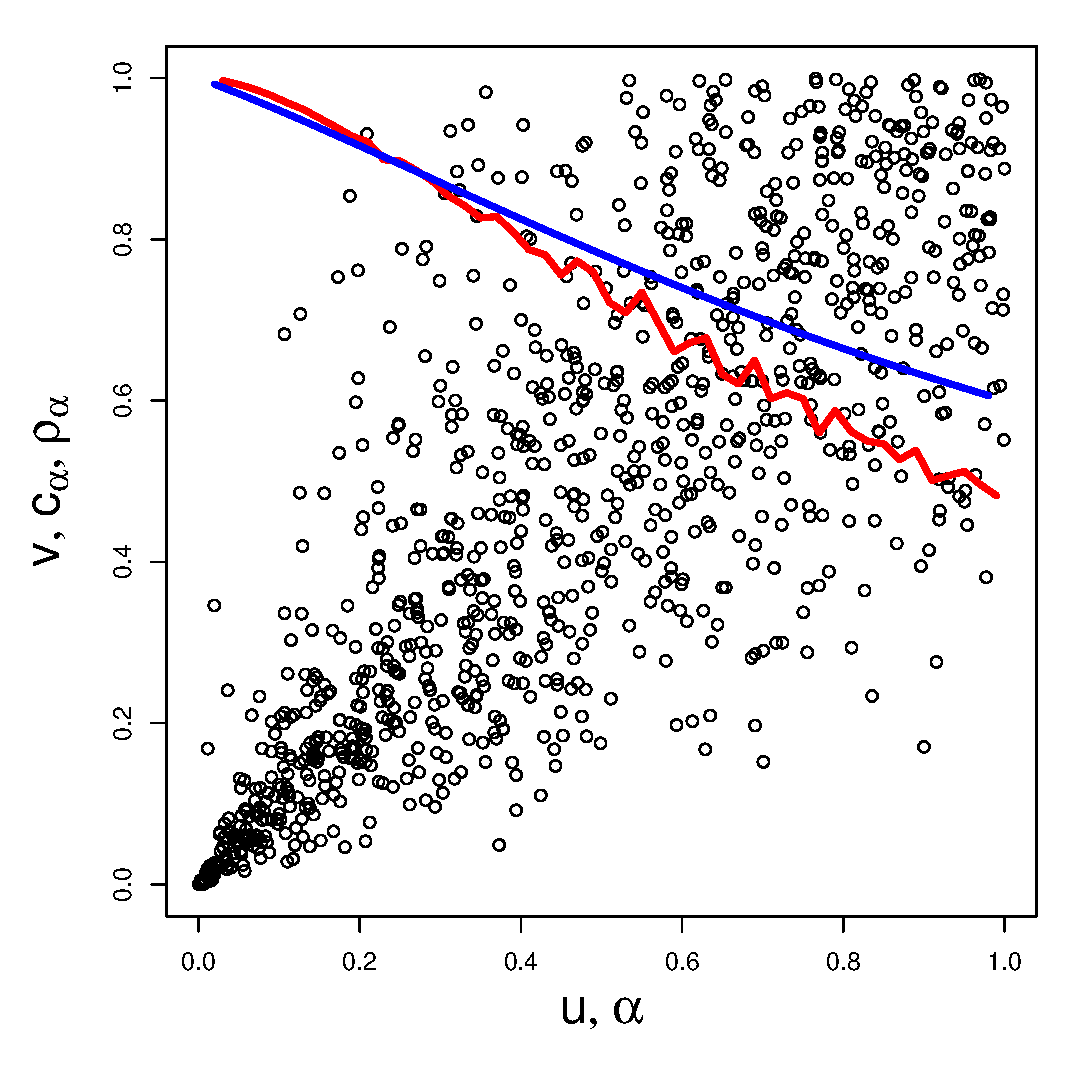
\includegraphics{cclayton.eps}}
      \resizebox{60mm}{!}{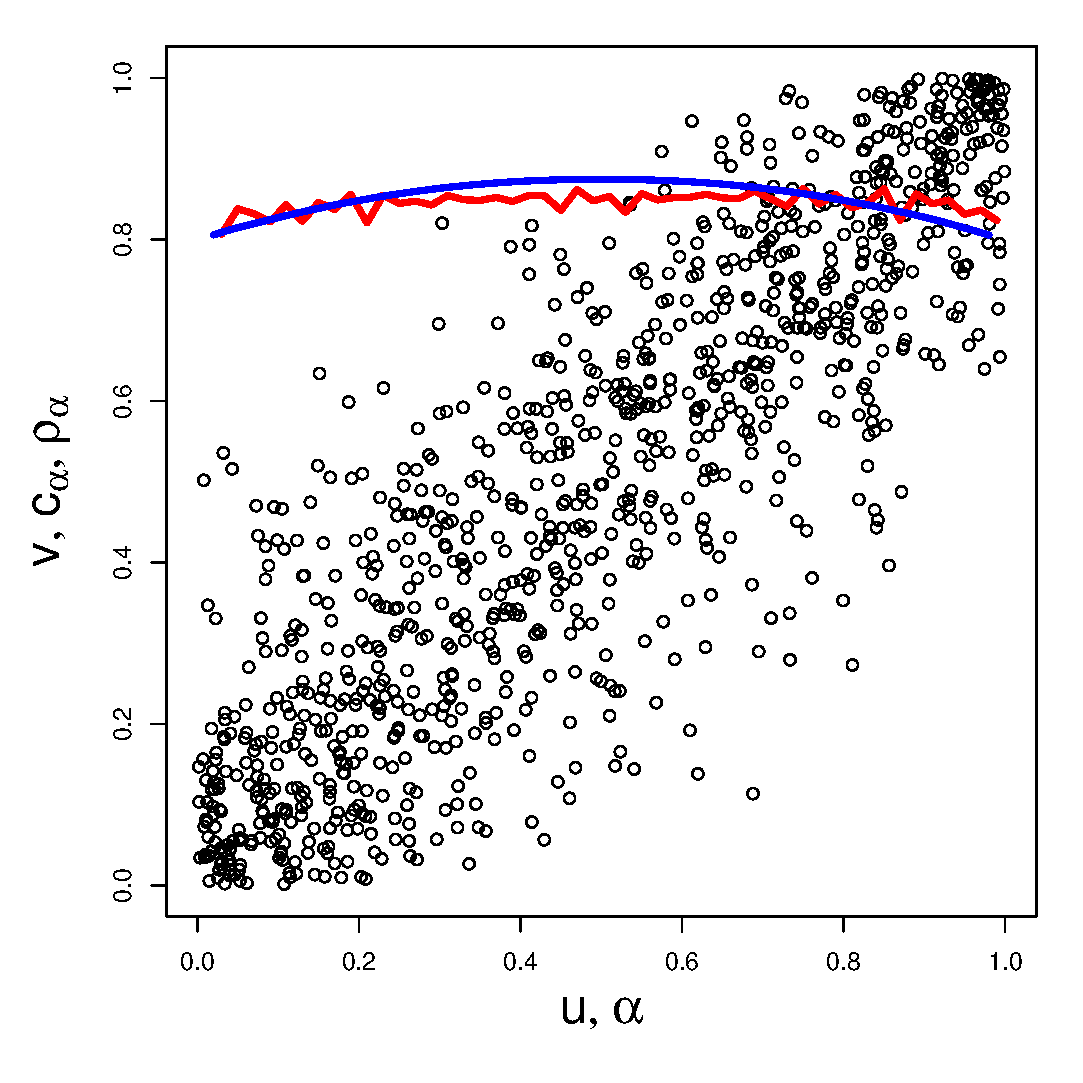
\includegraphics{cfrank.eps}} \\
    \end{tabular}
    \caption{Calculation of correlation curve (red line) for a Gaussian copula (top left), Gumbel copula (top right), Clayton copula (bottom left) and Frank copula (bottom right). Layer dependence (blue line) is also shown in each panel.}
    \label{fcorcurve}
  \end{center}
\end{figure}


\subsection{Bivariate local dependence measures}

\cite{bairamov2003new} defines a bivariate local dependence function, measuring dependence at various values of $(u,v)$, by generalising  $\rho+S$ using first and second order conditional expectations. \cite{jones1996local} and \cite{holland1987dependence} also define a bivariate local dependence function, based on partial derivatives of the log joint density function. Bivariate local dependence functions maintain the dimension of a bivariate joint distribution, and are less graphically interpretable than univariate local dependence functions such as layer dependence, tail concentration and correlation curve. In addition whilst the local dependence by \cite{bairamov2003new} is constrained in $[-1,1]$, the local dependence function by \cite{jones1996local} and \cite{holland1987dependence} is unconstrained and is $-\infty$ and $\infty$ for countermonotonic and comonotonic variables, respectively.


\end{comment}


\begin{comment}

\section{Generating factor copulas given layer dependence}


This section describes an algorithm to model a copula satisfying a given layer dependence function. The given layer dependence function may be estimated from past data, and possibly incorporate parametric smoothing and expert opinion. Non-linear regression copula models are assumed where layer dependence is controlled by the probability distribution of the systematic component relative to the noise component.

A non-linear regression copula model of $(u,v)$ is
\begin{equation}\label{regression}
v=\p\left\{S(u)+\epsilon\right\} \cq u\sim U(0,1) \cq \epsilon\sim N(0,1)
\end{equation}
where $u$ and $\epsilon$ are independent and $S$ is an increasing function. $\p$ represents the probability integral transform, hence $(u,v)$ is bivariate uniform. Call $S(u)$ and $\epsilon$ systematic and noise components of the copula model, respectively. Specifying $S$ completes the copula model.

Intuitively, the volatility pattern of $S(u)$ controls layer dependence between $u$ and $v$. Measure the volatility of $S(u)$ at $u$ as the derivative $S'(u)$, the gap between adjacent percentiles. If $S(u)$ has high volatility in the upper tail then $S(u)$ dominates $v$ for large values of $u$, yielding strong layer dependence between $u$ and $v$ at high layers. Vice versa for the lower tail. If $S(u)$ has low volatility at all percentiles then $v$ is dominated by noise, resulting in weak dependence. Lastly if $S^-=c\Phi^-$ for some constant $c$, where $\Phi^-$ is the inverse distribution function of the standard normal, then systematic and noise components are both normally distributed, yielding a Gaussian copula.

The following derives $S$ to satisfy a ``target" layer dependence function $\ell_\alpha$. $S$ is specified either non-parametrically or parametrically. A non-parametric $S$ is specified over a large number of points in the unit interval, while a parametric $S$ is restricted to a class of functions. Once $S$ is specified, the copula model \eref{regression} is simulated by generating large samples of $u$ and $\epsilon$ and then calculating a sample of $v$ as the empirical distribution function of simulated $S(u)+\epsilon$.

A non-parametric $S$ is derived iteratively as follows. First generate large samples of $u$ and $\epsilon$. Without loss of generality, assume the $u$-sample is ordered and ``error free": $[u_1,\ldots,u_n]$ where $u_i=i/n$. Generate the $\epsilon$-sample $[\epsilon_1,\ldots,\epsilon_n]$ independently of the $u$-sample. The aim is to derive an $S$-sample $[s_1,\ldots,s_n]$ where $s_i=S(u_i)=S(i/n)$ such that the resulting layer dependence function is $\ell_\alpha$. Initialise the $S$-sample by for example setting $s_i^1=c\Phi^-(u_i)$ where $c$ is a constant selected to achieve equal  $\rho_S$ as $\ell_\alpha$. Repeat the following steps for $t=1,2,\ldots$, until convergence:
\begin{enumerate}
\item At iteration $t$, update the $v$-sample by setting $v_i^t=\R(s_i^t+\epsilon_i)$ where $\R$ computes percentile ranks lying in the unit interval.
\newline

\item Compute the ``fitted" layer dependence function $\hat{\ell}_\alpha$ for the current $(u,v)$-sample, at all values of $\alpha$ in the $u$-sample.
\newline

\item Compute first order differences of the $S$-sample: $[d_1^t,\ldots d_{n-1}^t]$ where $d_i^t=s_{i+1}^t-s_i^t$, representing volatility of the systematic component.
\newline

\item Update first order differences based on the corresponding gap between target and fitted layer dependence functions: $d_i^{t+1}=d_i^t \times (\ell_{i/n}/\hat{\ell}_{i/n})^a$ where $a$ is the adjustment sensitivity, say $2$.
\newline

\item Update the $S$-sample by combining updated first order differences: $s_{i+1}^{t+1}=s_i^{t+1}+d_i^{t+1}$. The first value of the $S$-sample remains unchanged: $s_1^{t+1}=s_1^t$.

\end{enumerate}
At points where the target layer dependence exceeds fitted layer dependence, volatility of $S$ at the same point is increased so that the systematic component increases its dominance over the noise component. Vice versa where target layer dependence falls below fitted layer dependence. Therefore $S$ is iteratively ``re-shaped" depending on the gap between target and fitted layer dependence until the gap is satisfactorily small.

A parametric $S$ is derived by first restricting $S$ to a class of increasing functions, for example $S=G^-_\theta$ where $\theta$ is a set of parameters. Given $\theta$, a $(u,v)$-sample is simulated yielding a fitted layer dependence function $\hat{\ell}_\alpha$. The optimal $S$ is based on the value of $\theta$ minimising the gap between target layer and fitted dependence functions. The gap may be formulated for example as the ``mean square error" $\sum (\ell_\alpha-\hat{\ell}_\alpha)^2$ where the sum applies to a large range of values of $\alpha$ in the unit interval.

Non-parametric $S$ generally achieves superior fit to the target layer dependence function, compared to parametric $S$. In addition the copula model \eref{regression} generally does not permit closed form applications and hence simulation is required. In this case non-parametric $S$ performs equally, if not better, than parametric $S$.


\end{comment}



\begin{comment}
\section{Generalised layer dependence}\label{sgeneral}

This section generalises layer dependence in \eref{definition} by considering conditional tail expectations of transformed percentile ranks. Depending on the transformation, generalised layer dependence captures different aspects of dependence.

Define generalised $\alpha$-layer dependence as
\begin{equation}\label{generalgap}
\ell_\alpha^\phi \equiv \frac{\E\{\phi(v)|u>\alpha\}-\E\{\phi(v)|u\leq\alpha\}}{\E\{\phi(u)|u>\alpha\}-\E\{\phi(u)|u\leq\alpha\}}
=\frac{\cov\{\phi(v),(u>\alpha)\}}{\cov\{\phi(u),(u> \alpha)\}} \;,
\end{equation}
where $\phi$ is an increasing function. Generalised layer dependence evaluates conditional tail expectations of transformed percentile ranks $\phi(v)$ and $\phi(u)$, instead of $u$ and $v$ for original layer dependence. Setting $\phi(v)=v$ yields original layer dependence. Two examples of generalised layer dependence are shown below.

Similar to original layer dependence, generalised layer dependence can be expressed in terms of only upper or lower conditional tail expectations:
$$
\ell_\alpha^\phi = \frac{\E\{\phi(v)|u>\alpha\}-\E\{\phi(v)\}}{\E\{\phi(u)|u>\alpha\}-\E\{\phi(u)\}}
=\frac{\E\{\phi(v)|u\leq\alpha\}-\E\{\phi(v)\}}{\E\{\phi(u)|u\leq\alpha\}-\E\{\phi(u)\}} \;.
$$
Further re-writing generalised layer dependence in \eref{generalgap} yields
$$
\ell_\alpha^\phi = \frac{\E(v_*|u_*\geq \alpha_*)-\E(v_*|u_*\leq \alpha_*)}{\E(u_*|u_*\geq \alpha_*)-\E(u_*|u_*\leq \alpha_*)} \;,
$$
where
$$
u_*\equiv \phi(u) \cq v_*\equiv \phi(v) \cq \alpha_*\equiv \phi(\alpha) \;.
$$
Hence generalised layer dependence follows the same structure as percentile rank gap in \eref{definition}. However calculations are performed in the transformed $\phi$-space.

Generalised $\alpha$-layer dependence in general does not satisfy all coherence properties of original layer dependence in \sref{scoherence}. Independence and ordering properties hold for all transformations $\phi$. In addition $\ell_\alpha^\phi\leq 1$ in general, with equality if $u$ and $v$ are comonotonic. Symmetry holds if $\phi(1-v)=k-\phi(v)$ for any constant $k$, since this implies $\cov\{\phi(1-v),(u>\alpha)\}=-\cov\{\phi(v),(u>\alpha)\}$, hence the sign of generalised layer dependence switches if $u$ or $v$ is ranked in reverse order. Symmetry implies $\ell_\alpha^\phi=-1$ if $u$ and $v$ are countermonotonic, hence the bounds property holds.

As the following two examples illustrate, generalised layer dependence measures local dependence from different aspects.

\subsection{Stepped transformation}

Suppose $\phi(v)=(v>c)$ for $0\leq c\leq 1$. Hence transformed percentile rank is $1$ if percentile rank exceeds $c$, and zero otherwise. Generalised layer dependence is
$$
\ell_\alpha^\phi  = \frac{\cov\{(v>c),(u>\alpha)\}}{\cov\{(u>c),(u>\alpha)\}}
= \frac{\p(u>\alpha,v>c)-\p(u>\alpha)\p(v>c)}{\p(u>\alpha,u>c)-\p(u>\alpha)\p(u>c)}
$$
$$
= \frac{\p(u\leq\alpha,v\leq c)-\p(u\leq \alpha)\p(v\leq c)}{\p(u\leq\alpha,u\leq c)-\p(u\leq \alpha)\p(u\leq c)}
= \frac{C(\alpha,c)-\alpha c}{\min(\alpha,c)-\alpha c} \;.
$$
Hence local dependence in this case is based on the scaled excess of joint probabilities over the product of corresponding marginal probabilities. A higher scaled excess implies stronger local dependence, and vice versa. Zero scaled excess indicates $u$ and $v$ are independent in terms of probabilities, relative to $\alpha$.

Suppose $\ell_\alpha^\phi$ is specified for all $0\leq \alpha, c\leq 1$. Then the joint distribution of $(u,v)$ is specified completely: $C(\alpha,c)=\{\min(\alpha,c)-\alpha c\}\ell_\alpha^\phi+\alpha c$.

Taking a weighted average of $\ell_\alpha^\phi$ over all $c$ yields original $\alpha$-layer dependence:
$$
\int_0^1 w_c \ell_\alpha^\phi \de c = \ell_\alpha \cq c_k\equiv \frac{\min(\alpha,c)-\alpha c}{\int_0^1\min(\alpha,C)-\alpha c \de c}
=\frac{\min(\alpha,c)-\alpha c}{\frac{1}{2}\alpha(1-\alpha)} \;.
$$
The averaging of $\ell_\alpha^\phi$ over $c$ causes $\alpha$-layer dependence to be non-unique (see \sref{sother}), as the joint distribution of $(u,v)$ is completely specified only if $\ell_\alpha^\phi$ is given for all $c$.


\subsection{Power transformation}

Suppose $\phi(v)=v^n$ where $n\geq 1$. Generalised layer dependence is
$$
\ell_\alpha^\phi= \frac{\cov\{v^n,(u>\alpha)\}}{\cov\{u^n,(u>\alpha)\}} = \frac{\E(v^n|u>\alpha)-\frac{1}{n+1}}{\E(u^n|u>\alpha)-\frac{1}{n+1}}
=\frac{\E(v^n|u\leq\alpha)-\frac{1}{n+1}}{\E(u^n|u\leq\alpha)-\frac{1}{n+1}} \;.
$$
Local dependence in this case is based on conditional tail expectations of percentile rank powers. Setting $n=1$ yields original layer dependence $\ell_\alpha$.

Suppose $\ell_\alpha^\phi$ is specified for all $n\geq 1$. Then the conditional distribution of $v$ given $u>\alpha$ or given $u\leq \alpha$ is specified completely. The conditional distribution in turn yields the joint distribution of $(u,v)$.

\subsection{Graphical illustration}

\fref{fgeneral} calculates generalised layer dependence using the power transformation $\phi(v)=v^n$, using a Clayton copula identical to \fref{fillustration} and three values of $n$. Original layer dependence is also shown. The top left panel graphs in the original percentile rank scale, while remaining panels use power transformed percentile rank scales for different values of $n$.

From the top left panel, increasing $n$ emphasizes dependence over lower percentiles and diminishes dependence over larger percentiles. From the remaining panels, generalised layer dependence is more reflective of local dependence between $(u^n,v^n)$. Generalised layer dependence decreases more rapidly over higher percentiles reflecting weak upper tail dependence whereas original layer dependence decreases only gradually.

\begin{figure}
  \begin{center}
    \begin{tabular}{cc}
      \resizebox{60mm}{!}{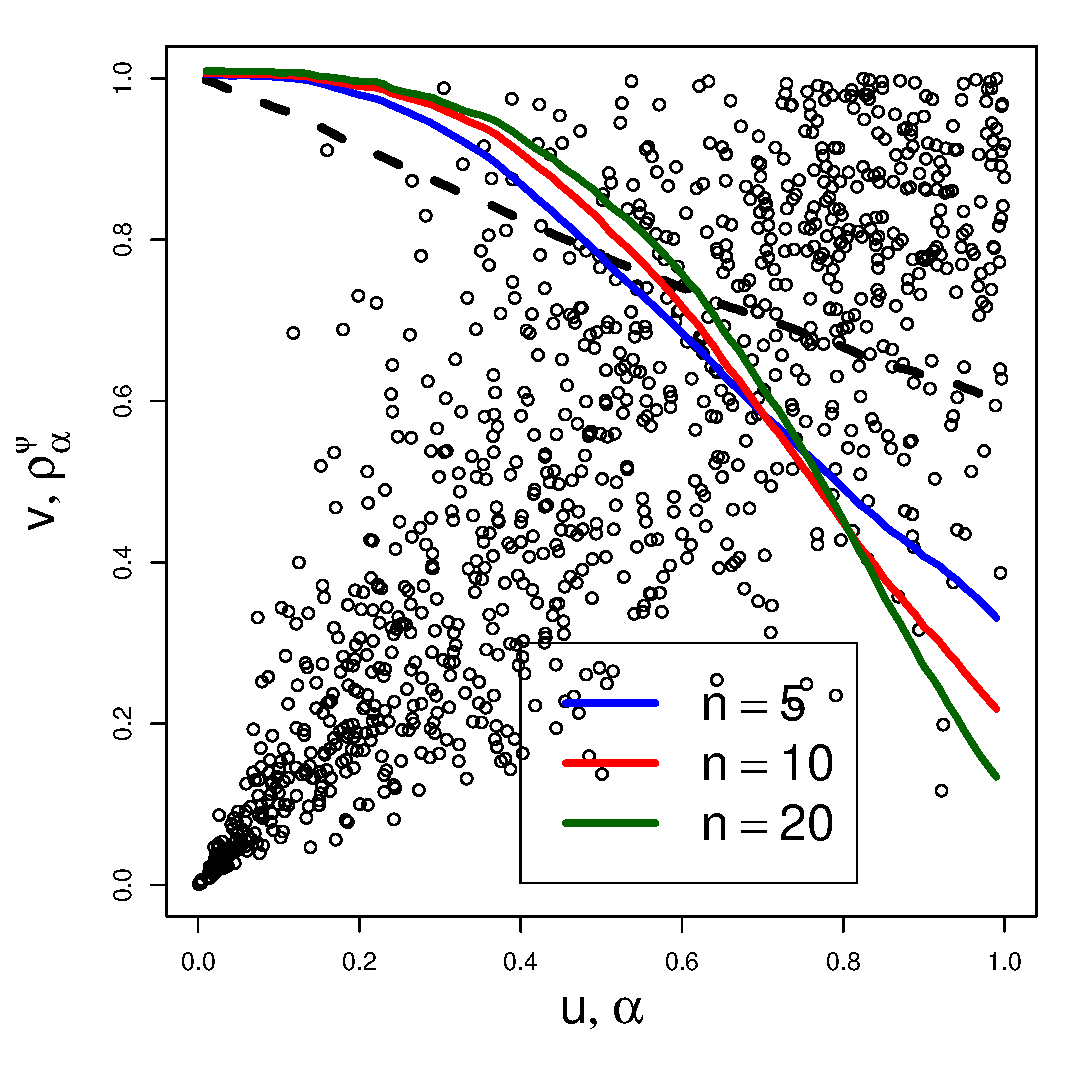
\includegraphics{eml.eps}}
      \resizebox{60mm}{!}{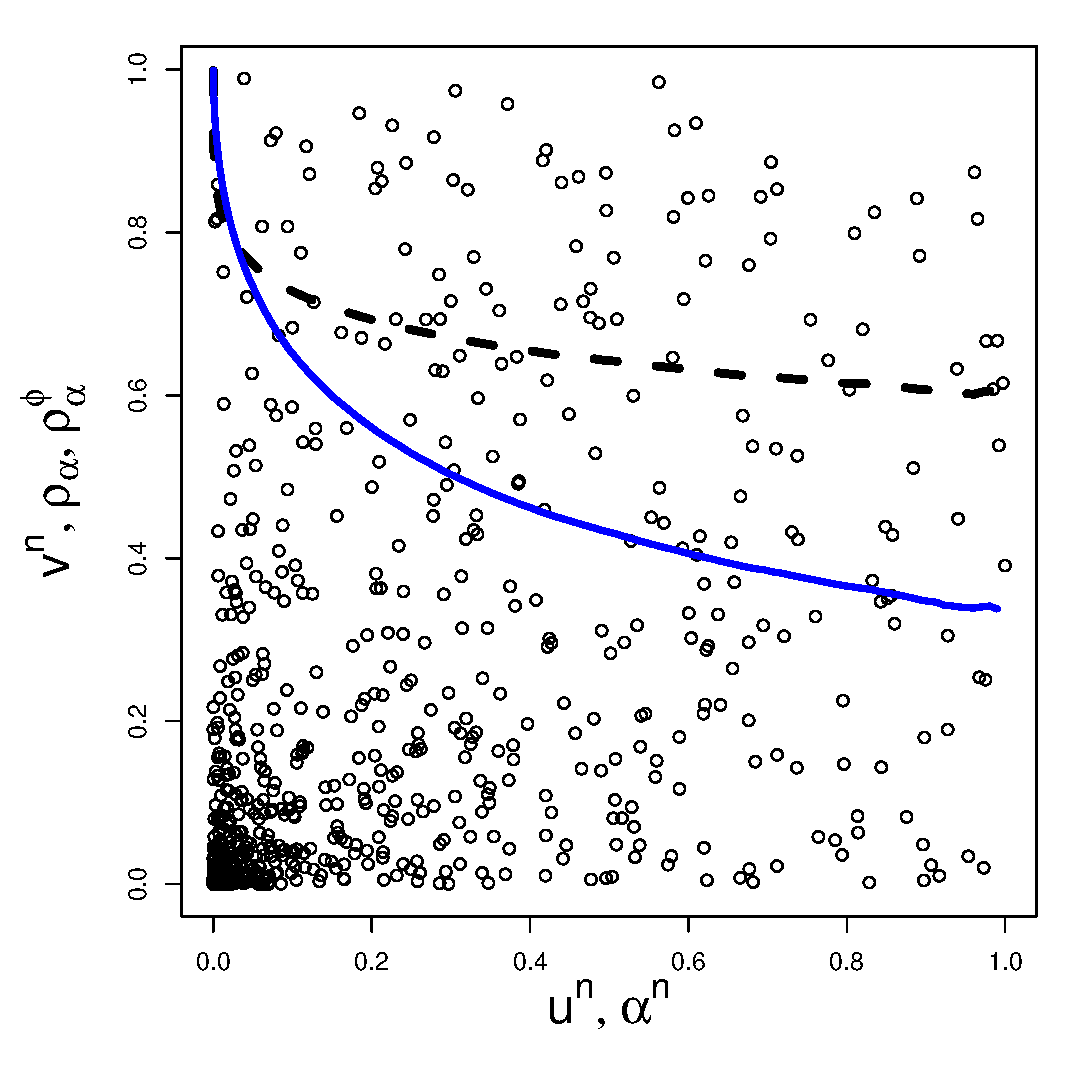
\includegraphics{eml1.eps}} \\
      \resizebox{60mm}{!}{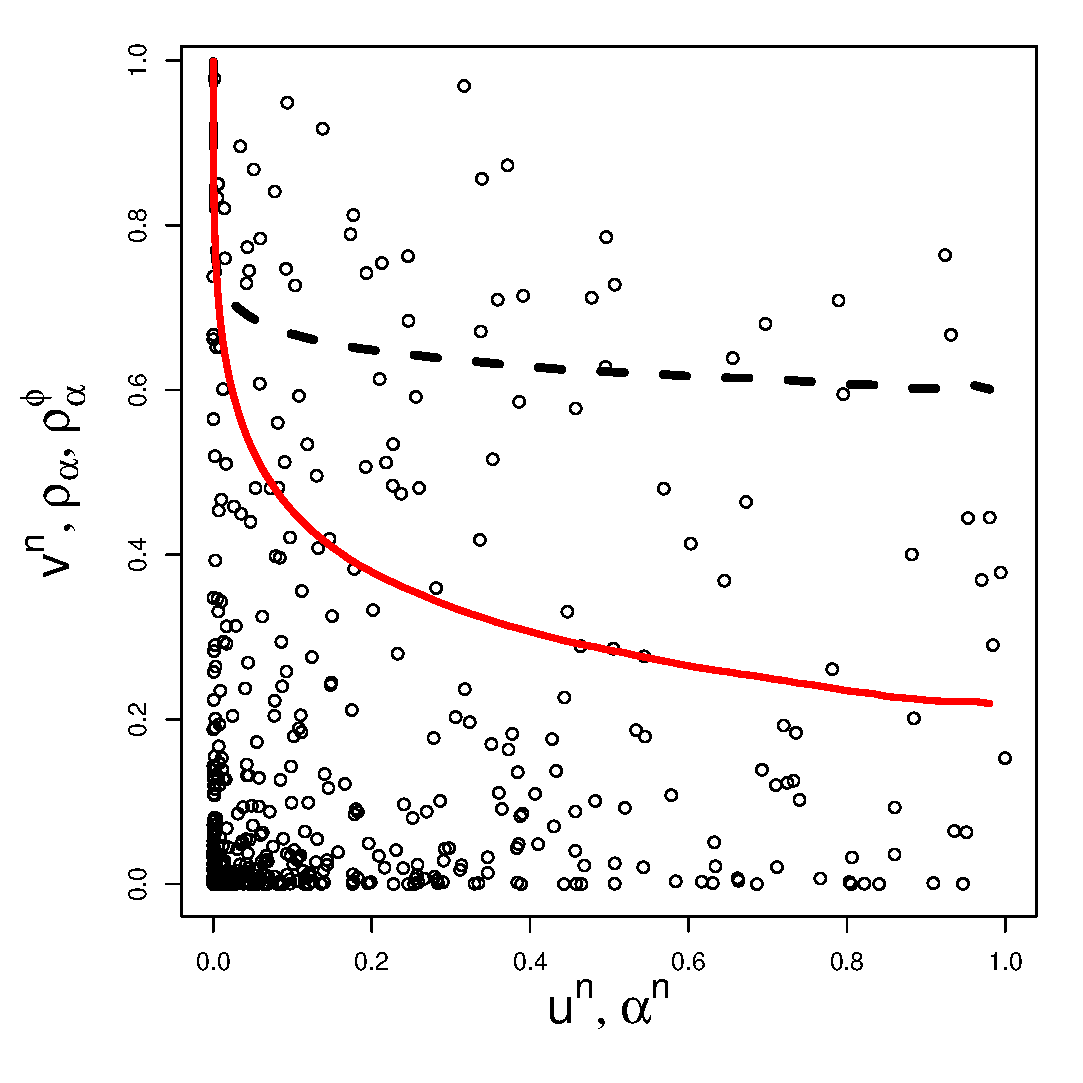
\includegraphics{eml2.eps}}
      \resizebox{60mm}{!}{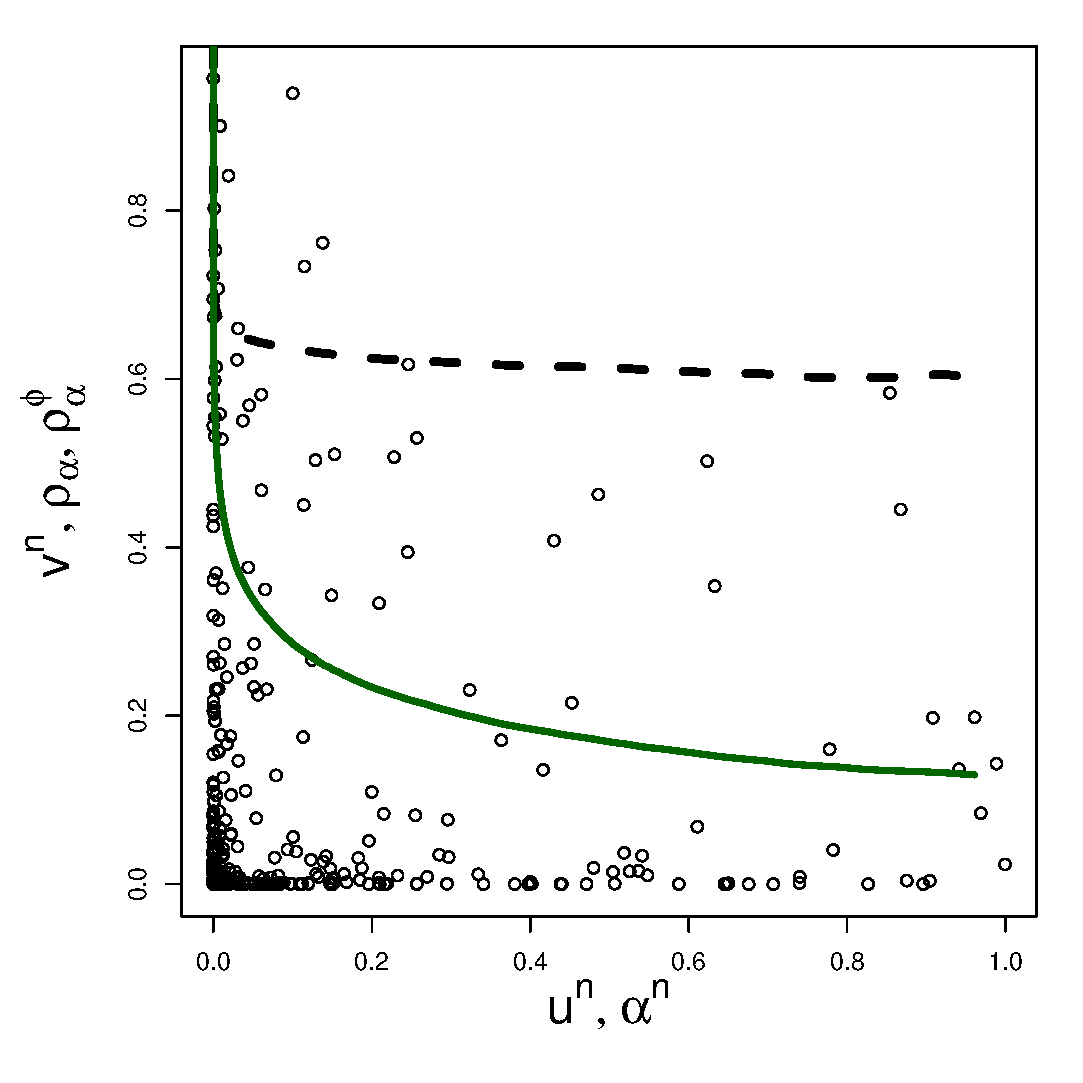
\includegraphics{eml3.eps}} \\
    \end{tabular}
    \caption{Calculation of generalised layer dependence (coloured lines) assuming $\phi(v)=v^n$ for $n=5$, $10$ and $20$, based on a Clayton copula. Original layer dependence is represented by dotted lines. The top left panel uses the original percentile rank gap, while remaining panels uses the transformed percentile rank gap scale for each value of $n$.}
    \label{fgeneral}
  \end{center}
\end{figure}

\end{comment}



\section{Conclusion}\label{sconclusion}

Layer dependence accurately captures dependence structures in bivariate copulas, and satisfies coherence properties. Taking weighted averages of layer dependence curves yields Spearman's correlation and alternative overall dependence measures.

Using layer dependence in copula fitting captures dependence structures in past data, whilst flexibly accommodating expert opinion. Layer dependence achieves a balance between parametric approaches (smooth fit, low flexibility) and empirical approaches (volatile fit, high flexibility).


\newpage


\begin{comment}

\subsection{Simulating constant layer dependence}\label{pconstant}


The following details an approach to simulate $(u,v)$ with constant layer dependence $\ell_\alpha=r$ where $0\leq r\leq 0.5$. First simulate bivariate uniform $(u_*,v_*)$ as
$$
(u_*,v_*)=(z\leq c) \times \{(u_0,v_0)\times c\} +(z>c)\times \{(c,c)+(u_0,v_0)\times (1-c)\}
$$
where $z$, $c$, $u_0$ and $v_0$ are independent uniform. Direct calculation shows the layer dependence of $(u_*,v_*)$ is constant and equal to $0.5$. Hence model $(u,v)$ as a mixture of independent uniform random variables and $(u_*,v_*)$, with weights $1-2r$ and $2r$, respectively. The layer dependence of $(u,v)$ is $(1-2r)\times 0+2r\times 0.5=r$, as desired.
\end{comment}


\newpage

\bibliography{PhD}





\end{document}
